%% PRD paper, first complete draft (16 Nov 2026).
%% Numbers are macros of values/results_macros.tex (written by scripts/build_values.py):
%%   red  (\ph)  = not yet computable (placeholders.txt, runs.txt)
%%   teal (\anc) = real, from the exploratory runs; the production runs replace it
%%   plain       = design choices and inputs of the simulated catalogs
%% Numbers the text needs and the macro file lacks are declared below with
%% \providecommand, so that a macro of the same name added to
%% values/results_macros.tex takes over without any edit here. They are listed in
%% notes/MACRO_REQUESTS.md.
\documentclass[aps,prd,reprint,twocolumn,superscriptaddress,nofootinbib,floatfix]{revtex4-2}

\usepackage{amsmath,amssymb}
\usepackage{graphicx}
\usepackage{xcolor}
\usepackage[colorlinks=true,linkcolor=blue,citecolor=blue,urlcolor=blue]{hyperref}

%% results_macros.tex -- written by scripts/build_values.py; do not edit by hand.
%% RED (\ph):   not computable from the stored results; see placeholders.txt for the run that produces it.
%% TEAL (\anc): a real number from the exploratory runs under working/analyses/; the production runs replace it.
%% Plain:       design choices and inputs of the simulated catalogs (working/data).
%% Every macro is traced in values/values.json (source file and key, or the computation).
\definecolor{phred}{rgb}{0.80,0.05,0.05}
\definecolor{ancteal}{rgb}{0.00,0.45,0.45}
\newcommand{\ph}[1]{\textcolor{phred}{#1}}
\newcommand{\anc}[1]{\textcolor{ancteal}{#1}}

%% ---- simulated catalogs: design choices and inputs (plain) ----
%% mock
\newcommand{\MockHzero}{67.74}  % input Hubble constant
\newcommand{\MockOmegam}{0.3075}  % input matter density Omega_m (fixed in every analysis)
\newcommand{\MockfAGN}{0.30}  % input fraction of mergers hosted by AGN
\newcommand{\MockfAGNRealised}{0.295}  % realised AGN-hosted fraction of the 1000 detected events of the reference catalog
\newcommand{\MocknGal}{10^{-3}}  % comoving number density of the galaxy catalog
\newcommand{\MocknAGN}{10^{-5}}  % comoving number density of the AGN catalog
\newcommand{\MockLognGal}{-3.0}  % log10 of the galaxy number density (input of the free-abundance analysis)
\newcommand{\MockLognAGN}{-5.0}  % log10 of the AGN number density
\newcommand{\MockbGal}{1.2}  % linear bias of the galaxies
\newcommand{\MockbAGN}{2.0}  % linear bias of the AGN
\newcommand{\MockLcut}{1.09}  % luminosity cut of the galaxy sample, L > x L* (B-band Schechter function)
\newcommand{\MockMBcut}{-20.56}  % absolute B magnitude of the galaxy cut
\newcommand{\MockLXcut}{43.7}  % AGN class: log10 L_X(2-10 keV) above this value (pinned literature density)
\newcommand{\MockNGal}{1.5\times10^{8}}  % realised galaxies to z = 1 (151,179,870)
\newcommand{\MockNAGN}{1.5\times10^{6}}  % realised AGN to z = 1 (1,514,567)
\newcommand{\MockzCat}{1}  % redshift depth of the catalogs
\newcommand{\MockDz}{0.003}  % catalog redshift error sigma_z = this value times (1+z)
\newcommand{\MockNside}{32}  % HEALPix nside of the catalog pixelisation
\newcommand{\MockNev}{1000}  % detected mergers per simulated catalog
\newcommand{\MockNsamp}{2000}  % posterior samples per event
\newcommand{\MockSNRthr}{8}  % detection threshold on the observed signal-to-noise ratio
\newcommand{\MockzHorizon}{0.31}  % largest true redshift of a detected event, reference catalog (the horizon)
\newcommand{\MockzMedian}{0.13}  % median redshift of the detected events, reference catalog
\newcommand{\MockzHorizonMin}{0.31}  % smallest horizon over the 9 catalogs of the joint analysis
\newcommand{\MockzHorizonMax}{0.39}  % largest horizon over the 9 catalogs of the joint analysis
\newcommand{\MockSkyMin}{1.0}  % smallest one-sigma sky localisation width, reference catalog
\newcommand{\MockSkyMax}{2.4}  % largest one-sigma sky localisation width, reference catalog
\newcommand{\MockSigLnMc}{0.08}  % chirp-mass error: sigma(ln Mc) = this value times 8/rho_obs
\newcommand{\MockSigLnq}{0.60}  % mass-ratio error: sigma(ln q) = this value times 8/rho_obs
\newcommand{\MockSigChi}{0.20}  % effective-spin error: sigma(chi_eff) = this value times 8/rho_obs
\newcommand{\MockMlimTwentyOne}{21}  % apparent-magnitude limit m < 21
\newcommand{\MockCompTwentyOne}{100.0}  % completeness of the galaxy catalog inside the horizon at m < 21 (AGN catalog: 100.0\%)
\newcommand{\MockMlimTwenty}{20}  % apparent-magnitude limit m < 20
\newcommand{\MockCompTwenty}{81.4}  % completeness of the galaxy catalog inside the horizon at m < 20 (AGN catalog: 81.4\%)
\newcommand{\MockMlimNineteen}{19}  % apparent-magnitude limit m < 19
\newcommand{\MockCompNineteen}{31.5}  % completeness of the galaxy catalog inside the horizon at m < 19 (AGN catalog: 31.7\%)
\newcommand{\MockMlimEighteen}{18}  % apparent-magnitude limit m < 18
\newcommand{\MockCompEighteen}{9.5}  % completeness of the galaxy catalog inside the horizon at m < 18 (AGN catalog: 9.6\%)
\newcommand{\MockAlpha}{2.3}  % power-law index of the primary mass
\newcommand{\MockMmin}{5}  % minimum mass
\newcommand{\MockMmax}{80}  % maximum mass
\newcommand{\MockPeakFrac}{0.90}  % fraction of the primary-mass distribution in the Gaussian peak
\newcommand{\MockMuG}{35}  % location of the Gaussian mass peak (galaxy hosts; both host classes in the common-population mocks)
\newcommand{\MockSigmaG}{5}  % width of the Gaussian mass peak
\newcommand{\MockBeta}{1}  % power-law index of the mass ratio
\newcommand{\MockMuChi}{0}  % mean effective spin (galaxy hosts)
\newcommand{\MockSigmaChi}{0.1}  % width of the effective-spin distribution
\newcommand{\MockGammaRate}{0}  % redshift evolution index of the merger rate, (1+z)^gamma
\newcommand{\MockDmuG}{5}  % input offset of the AGN mass-peak location (host-dependent mock)
\newcommand{\MockMuGAGN}{40}  % AGN mass-peak location in the host-dependent mock
\newcommand{\MockDmuChi}{0.10}  % input offset of the AGN mean effective spin
\newcommand{\MockHDNagn}{357}  % AGN-hosted events among the 1000 detected in the host-dependent mock
\newcommand{\MockHDfDet}{0.357}  % AGN-hosted fraction of the detected events in the host-dependent mock (heavier AGN mergers are louder; input 0.30)
\newcommand{\MockSpinNagn}{295}  % AGN-hosted events in the spin-offset-only mock (Analyses 8, 9)
\newcommand{\MockCtrlBranchFrac}{0.30}  % fraction of mergers drawn from the offset population in the galaxy-only control mock (all hosts galaxies)

%% ---- exploratory results (teal) ----
%% C1
\newcommand{\JointNcat}{\anc{9}}  % simulated catalogs with a complete joint (H0, f_AGN) grid on complete catalogs
\newcommand{\JointHzeroCatA}{\anc{69.2^{+1.6}_{-1.6}}}  % H0, complete catalogs, joint (H0, f_AGN) fit, catalog A (seed 100) (median and 90\% equal-tailed interval)
\newcommand{\JointHzeroCatAMed}{\anc{69.2}}  % median of H0, complete catalogs, joint (H0, f_AGN) fit, catalog A (seed 100)
\newcommand{\JointHzeroCatALo}{\anc{67.6}}  % lower end of the 90\% interval of H0, complete catalogs, joint (H0, f_AGN) fit, catalog A (seed 100)
\newcommand{\JointHzeroCatAHi}{\anc{70.8}}  % upper end of the 90\% interval of H0, complete catalogs, joint (H0, f_AGN) fit, catalog A (seed 100)
\newcommand{\JointfCatA}{\anc{0.273^{+0.078}_{-0.075}}}  % f_AGN, complete catalogs, joint fit, catalog A (seed 100) (median and 90\% equal-tailed interval)
\newcommand{\JointfCatAMed}{\anc{0.273}}  % median of f_AGN, complete catalogs, joint fit, catalog A (seed 100)
\newcommand{\JointfCatALo}{\anc{0.198}}  % lower end of the 90\% interval of f_AGN, complete catalogs, joint fit, catalog A (seed 100)
\newcommand{\JointfCatAHi}{\anc{0.352}}  % upper end of the 90\% interval of f_AGN, complete catalogs, joint fit, catalog A (seed 100)
\newcommand{\JointRhoCatA}{\anc{0.07}}  % correlation coefficient of H0 and f_AGN, catalog A (seed 100)
\newcommand{\JointHzeroCatB}{\anc{67.8^{+2.2}_{-2.0}}}  % H0, complete catalogs, joint (H0, f_AGN) fit, catalog B (seed 101) (median and 90\% equal-tailed interval)
\newcommand{\JointfCatB}{\anc{0.307^{+0.081}_{-0.077}}}  % f_AGN, complete catalogs, joint fit, catalog B (seed 101) (median and 90\% equal-tailed interval)
\newcommand{\JointRhoCatB}{\anc{0.23}}  % correlation coefficient of H0 and f_AGN, catalog B (seed 101)
\newcommand{\JointHzeroCatC}{\anc{66.5^{+1.9}_{-1.8}}}  % H0, complete catalogs, joint (H0, f_AGN) fit, catalog C (seed 102) (median and 90\% equal-tailed interval)
\newcommand{\JointfCatC}{\anc{0.247^{+0.085}_{-0.081}}}  % f_AGN, complete catalogs, joint fit, catalog C (seed 102) (median and 90\% equal-tailed interval)
\newcommand{\JointRhoCatC}{\anc{0.10}}  % correlation coefficient of H0 and f_AGN, catalog C (seed 102)
\newcommand{\JointHzeroCatD}{\anc{69.6^{+1.6}_{-1.5}}}  % H0, complete catalogs, joint (H0, f_AGN) fit, catalog D (seed 103) (median and 90\% equal-tailed interval)
\newcommand{\JointfCatD}{\anc{0.256^{+0.078}_{-0.074}}}  % f_AGN, complete catalogs, joint fit, catalog D (seed 103) (median and 90\% equal-tailed interval)
\newcommand{\JointRhoCatD}{\anc{0.03}}  % correlation coefficient of H0 and f_AGN, catalog D (seed 103)
\newcommand{\JointHzeroCatE}{\anc{67.6^{+1.7}_{-1.5}}}  % H0, complete catalogs, joint (H0, f_AGN) fit, catalog E (seed 105) (median and 90\% equal-tailed interval)
\newcommand{\JointfCatE}{\anc{0.352^{+0.083}_{-0.081}}}  % f_AGN, complete catalogs, joint fit, catalog E (seed 105) (median and 90\% equal-tailed interval)
\newcommand{\JointRhoCatE}{\anc{0.09}}  % correlation coefficient of H0 and f_AGN, catalog E (seed 105)
\newcommand{\JointHzeroCatF}{\anc{68.2^{+2.7}_{-2.7}}}  % H0, complete catalogs, joint (H0, f_AGN) fit, catalog F (seed 114) (median and 90\% equal-tailed interval)
\newcommand{\JointfCatF}{\anc{0.268^{+0.081}_{-0.077}}}  % f_AGN, complete catalogs, joint fit, catalog F (seed 114) (median and 90\% equal-tailed interval)
\newcommand{\JointRhoCatF}{\anc{0.03}}  % correlation coefficient of H0 and f_AGN, catalog F (seed 114)
\newcommand{\JointHzeroCatG}{\anc{67.7^{+1.9}_{-1.7}}}  % H0, complete catalogs, joint (H0, f_AGN) fit, catalog G (seed 115) (median and 90\% equal-tailed interval)
\newcommand{\JointfCatG}{\anc{0.330^{+0.082}_{-0.081}}}  % f_AGN, complete catalogs, joint fit, catalog G (seed 115) (median and 90\% equal-tailed interval)
\newcommand{\JointRhoCatG}{\anc{0.10}}  % correlation coefficient of H0 and f_AGN, catalog G (seed 115)
\newcommand{\JointHzeroCatH}{\anc{68.3^{+1.7}_{-1.7}}}  % H0, complete catalogs, joint (H0, f_AGN) fit, catalog H (seed 116) (median and 90\% equal-tailed interval)
\newcommand{\JointfCatH}{\anc{0.351^{+0.086}_{-0.085}}}  % f_AGN, complete catalogs, joint fit, catalog H (seed 116) (median and 90\% equal-tailed interval)
\newcommand{\JointRhoCatH}{\anc{0.15}}  % correlation coefficient of H0 and f_AGN, catalog H (seed 116)
\newcommand{\JointHzeroCatI}{\anc{69.3^{+2.2}_{-2.6}}}  % H0, complete catalogs, joint (H0, f_AGN) fit, catalog I (seed 117) (median and 90\% equal-tailed interval)
\newcommand{\JointfCatI}{\anc{0.154^{+0.083}_{-0.077}}}  % f_AGN, complete catalogs, joint fit, catalog I (seed 117) (median and 90\% equal-tailed interval)
\newcommand{\JointRhoCatI}{\anc{-0.05}}  % correlation coefficient of H0 and f_AGN, catalog I (seed 117)
\newcommand{\JointRhoMean}{\anc{0.08}}  % mean over the 9 catalogs of the H0-f_AGN correlation coefficient
\newcommand{\JointRhoMin}{\anc{-0.05}}  % smallest H0-f_AGN correlation coefficient over the 9 catalogs
\newcommand{\JointRhoMax}{\anc{0.23}}  % largest H0-f_AGN correlation coefficient over the 9 catalogs
\newcommand{\JointHzeroComb}{\anc{68.36^{+0.63}_{-0.63}}}  % H0, combined posterior of the 9 complete-catalog joint analyses (median and 90\% equal-tailed interval)
\newcommand{\JointHzeroCombMed}{\anc{68.36}}  % median of H0, combined posterior of the 9 complete-catalog joint analyses
\newcommand{\JointHzeroCombLo}{\anc{67.73}}  % lower end of the 90\% interval of H0, combined posterior of the 9 complete-catalog joint analyses
\newcommand{\JointHzeroCombHi}{\anc{69.00}}  % upper end of the 90\% interval of H0, combined posterior of the 9 complete-catalog joint analyses
\newcommand{\JointfComb}{\anc{0.283^{+0.027}_{-0.027}}}  % f_AGN, combined posterior of the 9 complete-catalog joint analyses (median and 90\% equal-tailed interval)
\newcommand{\JointfCombMed}{\anc{0.283}}  % median of f_AGN, combined posterior of the 9 complete-catalog joint analyses
\newcommand{\JointfCombLo}{\anc{0.256}}  % lower end of the 90\% interval of f_AGN, combined posterior of the 9 complete-catalog joint analyses
\newcommand{\JointfCombHi}{\anc{0.310}}  % upper end of the 90\% interval of f_AGN, combined posterior of the 9 complete-catalog joint analyses
\newcommand{\JointHzeroCombLevel}{\anc{89}}  % two-sided credible level at which the input H0 = 67.74 lies in the combined complete-catalog posterior
\newcommand{\JointfCombLevel}{\anc{70}}  % two-sided credible level at which the input f_AGN = 0.30 lies in the combined complete-catalog posterior
\newcommand{\JointCombLevelTwoD}{\anc{88}}  % credible level of the highest-density 2-D region of the combined (H0, f_AGN) posterior whose boundary passes through the input point
\newcommand{\JointRhoComb}{\anc{0.11}}  % H0-f_AGN correlation coefficient of the combined posterior
\newcommand{\JointLnLVarMax}{\anc{11.0}}  % largest over the 9 catalogs of the Monte Carlo variance of ln L (selection plus event terms) at the grid maximum
\newcommand{\JointLnLVarMin}{\anc{8.1}}  % smallest such variance over the 9 catalogs
%% C2
\newcommand{\GalOnlyHzeroCatA}{\anc{69.9^{+3.0}_{-2.7}}}  % H0 from all 1000 events with the galaxy catalog alone, catalog A (seed 100) (median and 90\% equal-tailed interval)
\newcommand{\GalOnlyHzeroCatAMed}{\anc{69.9}}  % median of H0 from all 1000 events with the galaxy catalog alone, catalog A (seed 100)
\newcommand{\GalOnlyHzeroCatALo}{\anc{67.2}}  % lower end of the 90\% interval of H0 from all 1000 events with the galaxy catalog alone, catalog A (seed 100)
\newcommand{\GalOnlyHzeroCatAHi}{\anc{72.9}}  % upper end of the 90\% interval of H0 from all 1000 events with the galaxy catalog alone, catalog A (seed 100)
\newcommand{\LBfZeroCatA}{\anc{11.1}}  % log10 Bayes factor of the two-population model against galaxy hosts only, Savage-Dickey at f_AGN = 0, catalog A (seed 100)
\newcommand{\LBfOneCatA}{\anc{357.6}}  % log10 Bayes factor of the two-population model against AGN hosts only, Savage-Dickey at f_AGN = 1, catalog A (seed 100)
\newcommand{\GalOnlyHzeroCatB}{\anc{69.0^{+5.2}_{-3.1}}}  % H0 from all 1000 events with the galaxy catalog alone, catalog B (seed 101) (median and 90\% equal-tailed interval)
\newcommand{\LBfZeroCatB}{\anc{12.6}}  % log10 Bayes factor of the two-population model against galaxy hosts only, Savage-Dickey at f_AGN = 0, catalog B (seed 101)
\newcommand{\LBfOneCatB}{\anc{258.1}}  % log10 Bayes factor of the two-population model against AGN hosts only, Savage-Dickey at f_AGN = 1, catalog B (seed 101)
\newcommand{\GalOnlyHzeroCatC}{\anc{66.0^{+4.1}_{-3.8}}}  % H0 from all 1000 events with the galaxy catalog alone, catalog C (seed 102) (median and 90\% equal-tailed interval)
\newcommand{\LBfZeroCatC}{\anc{5.97}}  % log10 Bayes factor of the two-population model against galaxy hosts only, Savage-Dickey at f_AGN = 0, catalog C (seed 102)
\newcommand{\LBfOneCatC}{\anc{101.0}}  % log10 Bayes factor of the two-population model against AGN hosts only, Savage-Dickey at f_AGN = 1, catalog C (seed 102)
\newcommand{\GalOnlyHzeroCatD}{\anc{73.4^{+3.6}_{-4.4}}}  % H0 from all 1000 events with the galaxy catalog alone, catalog D (seed 103) (median and 90\% equal-tailed interval)
\newcommand{\LBfZeroCatD}{\anc{11.0}}  % log10 Bayes factor of the two-population model against galaxy hosts only, Savage-Dickey at f_AGN = 0, catalog D (seed 103)
\newcommand{\LBfOneCatD}{\anc{269.7}}  % log10 Bayes factor of the two-population model against AGN hosts only, Savage-Dickey at f_AGN = 1, catalog D (seed 103)
\newcommand{\GalOnlyHzeroCatE}{\anc{67.2^{+3.2}_{-2.9}}}  % H0 from all 1000 events with the galaxy catalog alone, catalog E (seed 105) (median and 90\% equal-tailed interval)
\newcommand{\LBfZeroCatE}{\anc{14.4}}  % log10 Bayes factor of the two-population model against galaxy hosts only, Savage-Dickey at f_AGN = 0, catalog E (seed 105)
\newcommand{\LBfOneCatE}{\anc{184.6}}  % log10 Bayes factor of the two-population model against AGN hosts only, Savage-Dickey at f_AGN = 1, catalog E (seed 105)
\newcommand{\GalOnlyHzeroCatF}{\anc{69.4^{+4.9}_{-3.6}}}  % H0 from all 1000 events with the galaxy catalog alone, catalog F (seed 114) (median and 90\% equal-tailed interval)
\newcommand{\LBfZeroCatF}{\anc{9.45}}  % log10 Bayes factor of the two-population model against galaxy hosts only, Savage-Dickey at f_AGN = 0, catalog F (seed 114)
\newcommand{\LBfOneCatF}{\anc{223.5}}  % log10 Bayes factor of the two-population model against AGN hosts only, Savage-Dickey at f_AGN = 1, catalog F (seed 114)
\newcommand{\GalOnlyHzeroCatG}{\anc{69.3^{+5.3}_{-4.3}}}  % H0 from all 1000 events with the galaxy catalog alone, catalog G (seed 115) (median and 90\% equal-tailed interval)
\newcommand{\LBfZeroCatG}{\anc{12.8}}  % log10 Bayes factor of the two-population model against galaxy hosts only, Savage-Dickey at f_AGN = 0, catalog G (seed 115)
\newcommand{\LBfOneCatG}{\anc{241.6}}  % log10 Bayes factor of the two-population model against AGN hosts only, Savage-Dickey at f_AGN = 1, catalog G (seed 115)
\newcommand{\GalOnlyHzeroCatH}{\anc{68.2^{+3.6}_{-4.1}}}  % H0 from all 1000 events with the galaxy catalog alone, catalog H (seed 116) (median and 90\% equal-tailed interval)
\newcommand{\LBfZeroCatH}{\anc{15.9}}  % log10 Bayes factor of the two-population model against galaxy hosts only, Savage-Dickey at f_AGN = 0, catalog H (seed 116)
\newcommand{\LBfOneCatH}{\anc{173.5}}  % log10 Bayes factor of the two-population model against AGN hosts only, Savage-Dickey at f_AGN = 1, catalog H (seed 116)
\newcommand{\GalOnlyHzeroCatI}{\anc{69.8^{+2.7}_{-2.8}}}  % H0 from all 1000 events with the galaxy catalog alone, catalog I (seed 117) (median and 90\% equal-tailed interval)
\newcommand{\LBfZeroCatI}{\anc{1.82}}  % log10 Bayes factor of the two-population model against galaxy hosts only, Savage-Dickey at f_AGN = 0, catalog I (seed 117)
\newcommand{\LBfOneCatI}{\anc{203.2}}  % log10 Bayes factor of the two-population model against AGN hosts only, Savage-Dickey at f_AGN = 1, catalog I (seed 117)
\newcommand{\AgnOnlyNoInterior}{\anc{8}}  % number of the 9 catalogs whose AGN-catalog-only H0 posterior (all events) has no interior maximum in [50, 100] (log-likelihood largest at a grid edge)
\newcommand{\AgnOnlyHzeroCatC}{\anc{76.21^{+1.01}_{-0.81}}}  % H0 from all 1000 events with the AGN catalog alone, catalog C (seed 102), the one catalog whose AGN-only posterior has an interior maximum (median and 90\% equal-tailed interval)
\newcommand{\AgnOnlyArgmaxCatA}{\anc{100.0}}  % H0 at which the AGN-catalog-only log-likelihood (all events, catalog A) is largest; 100 is the top of the scanned range
\newcommand{\LBfZeroMin}{\anc{1.8}}  % smallest per-catalog log10 B (two populations against galaxy hosts only) over the 9 catalogs
\newcommand{\LBfZeroMax}{\anc{15.9}}  % largest per-catalog log10 B (two populations against galaxy hosts only)
\newcommand{\GalOnlyHzeroComb}{\anc{68.9^{+1.3}_{-1.3}}}  % H0 with the galaxy catalog alone (all events), combined over the 9 catalogs (median and 90\% equal-tailed interval)
\newcommand{\GalOnlyHzeroCombMed}{\anc{68.9}}  % median of H0 with the galaxy catalog alone (all events), combined over the 9 catalogs
\newcommand{\GalOnlyHzeroCombLo}{\anc{67.7}}  % lower end of the 90\% interval of H0 with the galaxy catalog alone (all events), combined over the 9 catalogs
\newcommand{\GalOnlyHzeroCombHi}{\anc{70.2}}  % upper end of the 90\% interval of H0 with the galaxy catalog alone (all events), combined over the 9 catalogs
\newcommand{\GalOnlyHzeroCombLevel}{\anc{88}}  % two-sided credible level of the input H0 in the combined galaxy-catalog-only posterior
\newcommand{\LBfZeroComb}{\anc{101.2}}  % log10 Bayes factor of the two-population model against galaxy hosts only, combined over the 9 catalogs (Savage-Dickey at f_AGN = 0 on the summed grid)
\newcommand{\LBfOneComb}{\anc{2037.9}}  % log10 Bayes factor of the two-population model against AGN hosts only, combined over the 9 catalogs (Savage-Dickey at f_AGN = 1)
%% C3
\newcommand{\PureNcat}{\anc{93}}  % simulated catalogs with both a 1000-event all-galaxy-host set and a 1000-event all-AGN-host set analysed
\newcommand{\PureGalHalfSixtyEight}{\anc{2.11}}  % mean over catalogs of the 68\% half-width of H0 from 1000 galaxy-hosted mergers
\newcommand{\PureAGNHalfSixtyEight}{\anc{0.45}}  % mean over catalogs of the 68\% half-width of H0 from 1000 AGN-hosted mergers
\newcommand{\PureGalHalfNinety}{\anc{3.53}}  % mean over catalogs of the 90\% half-width of H0, galaxy-hosted set
\newcommand{\PureAGNHalfNinety}{\anc{0.75}}  % mean over catalogs of the 90\% half-width of H0, AGN-hosted set
\newcommand{\PureRatioSixtyEight}{\anc{4.7}}  % ratio of the mean 68\% half-widths, galaxy-hosted over AGN-hosted
\newcommand{\PureRatioNinety}{\anc{4.7}}  % ratio of the mean 90\% half-widths, galaxy-hosted over AGN-hosted
\newcommand{\PureGalHzeroComb}{\anc{67.71^{+0.36}_{-0.35}}}  % H0, combined posterior of the 93 galaxy-hosted event sets (median and 90\% equal-tailed interval)
\newcommand{\PureGalHzeroCombMed}{\anc{67.71}}  % median of H0, combined posterior of the 93 galaxy-hosted event sets
\newcommand{\PureGalHzeroCombLo}{\anc{67.35}}  % lower end of the 90\% interval of H0, combined posterior of the 93 galaxy-hosted event sets
\newcommand{\PureGalHzeroCombHi}{\anc{68.06}}  % upper end of the 90\% interval of H0, combined posterior of the 93 galaxy-hosted event sets
\newcommand{\PureGalHzeroCombLevel}{\anc{12}}  % two-sided credible level of the input H0 in the combined galaxy-hosted posterior
\newcommand{\PureAGNHzeroComb}{\anc{67.820^{+0.080}_{-0.079}}}  % H0, combined posterior of the 93 AGN-hosted event sets (median and 90\% equal-tailed interval)
\newcommand{\PureAGNHzeroCombMed}{\anc{67.820}}  % median of H0, combined posterior of the 93 AGN-hosted event sets
\newcommand{\PureAGNHzeroCombLo}{\anc{67.741}}  % lower end of the 90\% interval of H0, combined posterior of the 93 AGN-hosted event sets
\newcommand{\PureAGNHzeroCombHi}{\anc{67.901}}  % upper end of the 90\% interval of H0, combined posterior of the 93 AGN-hosted event sets
\newcommand{\PureAGNHzeroCombLevel}{\anc{91}}  % two-sided credible level of the input H0 in the combined AGN-hosted posterior
%% C4
\newcommand{\FluxfHalfComplete}{\anc{0.077}}  % 90\% half-width of f_AGN with complete catalogs (reference catalog, C1 grid)
\newcommand{\FluxHzeroHalfComplete}{\anc{1.60}}  % 90\% half-width of H0 with complete catalogs (reference catalog, C1 grid)
\newcommand{\FluxHzeroTwentyOne}{\anc{69.2^{+1.6}_{-1.6}}}  % H0, flux limit m < 21, densities of missing hosts at their input values (median and 90\% equal-tailed interval)
\newcommand{\FluxfTwentyOne}{\anc{0.273^{+0.078}_{-0.075}}}  % f_AGN, flux limit m < 21, densities at input (median and 90\% equal-tailed interval)
\newcommand{\FluxfHalfTwentyOne}{\anc{0.077}}  % 90\% half-width of f_AGN at m < 21
\newcommand{\FluxHzeroHalfTwentyOne}{\anc{1.59}}  % 90\% half-width of H0 at m < 21
\newcommand{\FluxfRatioTwentyOne}{\anc{1.00}}  % 90\% half-width of f_AGN at m < 21 over that with complete catalogs (C1 grid, same catalog)
\newcommand{\FluxHzeroRatioTwentyOne}{\anc{1.00}}  % 90\% half-width of H0 at m < 21 over that with complete catalogs (C1 grid, same catalog)
\newcommand{\FluxfShiftTwentyOne}{\anc{0.000}}  % median f_AGN at m < 21 minus the complete-catalog median (same catalog)
\newcommand{\FluxHzeroShiftTwentyOne}{\anc{0.00}}  % median H0 at m < 21 minus the complete-catalog median (same catalog)
\newcommand{\FluxHzeroTwenty}{\anc{69.2^{+1.6}_{-1.6}}}  % H0, flux limit m < 20, densities of missing hosts at their input values (median and 90\% equal-tailed interval)
\newcommand{\FluxfTwenty}{\anc{0.273^{+0.078}_{-0.075}}}  % f_AGN, flux limit m < 20, densities at input (median and 90\% equal-tailed interval)
\newcommand{\FluxfHalfTwenty}{\anc{0.077}}  % 90\% half-width of f_AGN at m < 20
\newcommand{\FluxHzeroHalfTwenty}{\anc{1.60}}  % 90\% half-width of H0 at m < 20
\newcommand{\FluxfRatioTwenty}{\anc{1.00}}  % 90\% half-width of f_AGN at m < 20 over that with complete catalogs (C1 grid, same catalog)
\newcommand{\FluxHzeroRatioTwenty}{\anc{1.00}}  % 90\% half-width of H0 at m < 20 over that with complete catalogs (C1 grid, same catalog)
\newcommand{\FluxfShiftTwenty}{\anc{0.000}}  % median f_AGN at m < 20 minus the complete-catalog median (same catalog)
\newcommand{\FluxHzeroShiftTwenty}{\anc{0.00}}  % median H0 at m < 20 minus the complete-catalog median (same catalog)
\newcommand{\FluxHzeroNineteen}{\anc{69.0^{+1.6}_{-1.6}}}  % H0, flux limit m < 19, densities of missing hosts at their input values (median and 90\% equal-tailed interval)
\newcommand{\FluxfNineteen}{\anc{0.275^{+0.079}_{-0.076}}}  % f_AGN, flux limit m < 19, densities at input (median and 90\% equal-tailed interval)
\newcommand{\FluxfHalfNineteen}{\anc{0.078}}  % 90\% half-width of f_AGN at m < 19
\newcommand{\FluxHzeroHalfNineteen}{\anc{1.62}}  % 90\% half-width of H0 at m < 19
\newcommand{\FluxfRatioNineteen}{\anc{1.01}}  % 90\% half-width of f_AGN at m < 19 over that with complete catalogs (C1 grid, same catalog)
\newcommand{\FluxHzeroRatioNineteen}{\anc{1.01}}  % 90\% half-width of H0 at m < 19 over that with complete catalogs (C1 grid, same catalog)
\newcommand{\FluxfShiftNineteen}{\anc{0.002}}  % median f_AGN at m < 19 minus the complete-catalog median (same catalog)
\newcommand{\FluxHzeroShiftNineteen}{\anc{-0.26}}  % median H0 at m < 19 minus the complete-catalog median (same catalog)
\newcommand{\FluxHzeroEighteen}{\anc{68.7^{+1.6}_{-1.8}}}  % H0, flux limit m < 18, densities of missing hosts at their input values (median and 90\% equal-tailed interval)
\newcommand{\FluxfEighteen}{\anc{0.286^{+0.083}_{-0.080}}}  % f_AGN, flux limit m < 18, densities at input (median and 90\% equal-tailed interval)
\newcommand{\FluxfHalfEighteen}{\anc{0.082}}  % 90\% half-width of f_AGN at m < 18
\newcommand{\FluxHzeroHalfEighteen}{\anc{1.71}}  % 90\% half-width of H0 at m < 18
\newcommand{\FluxfRatioEighteen}{\anc{1.06}}  % 90\% half-width of f_AGN at m < 18 over that with complete catalogs (C1 grid, same catalog)
\newcommand{\FluxHzeroRatioEighteen}{\anc{1.07}}  % 90\% half-width of H0 at m < 18 over that with complete catalogs (C1 grid, same catalog)
\newcommand{\FluxfShiftEighteen}{\anc{0.013}}  % median f_AGN at m < 18 minus the complete-catalog median (same catalog)
\newcommand{\FluxHzeroShiftEighteen}{\anc{-0.55}}  % median H0 at m < 18 minus the complete-catalog median (same catalog)
%% C5
\newcommand{\SlopefAGNTwentyOne}{\anc{0.43}}  % d f_AGN / d log10 n_AGN at m < 21 (assumed AGN density of missing hosts varied by factors 0.5 to 2)
\newcommand{\SlopeHzeroTwentyOne}{\anc{-0.02}}  % d H0 / d log10 n_AGN at m < 21
\newcommand{\DeltafTwoTwentyOne}{\anc{0.13}}  % change of f_AGN for a factor of two in the assumed AGN density at m < 21 (slope times log10 2)
\newcommand{\DeltaHzeroTwoTwentyOne}{\anc{-0.01}}  % change of H0 for a factor of two in the assumed AGN density at m < 21 (slope times log10 2)
\newcommand{\SlopefAGNTwenty}{\anc{0.44}}  % d f_AGN / d log10 n_AGN at m < 20 (assumed AGN density of missing hosts varied by factors 0.5 to 2)
\newcommand{\SlopeHzeroTwenty}{\anc{-0.03}}  % d H0 / d log10 n_AGN at m < 20
\newcommand{\DeltafTwoTwenty}{\anc{0.13}}  % change of f_AGN for a factor of two in the assumed AGN density at m < 20 (slope times log10 2)
\newcommand{\DeltaHzeroTwoTwenty}{\anc{-0.01}}  % change of H0 for a factor of two in the assumed AGN density at m < 20 (slope times log10 2)
\newcommand{\SlopefAGNNineteen}{\anc{0.47}}  % d f_AGN / d log10 n_AGN at m < 19 (assumed AGN density of missing hosts varied by factors 0.5 to 2)
\newcommand{\SlopeHzeroNineteen}{\anc{0.71}}  % d H0 / d log10 n_AGN at m < 19
\newcommand{\DeltafTwoNineteen}{\anc{0.14}}  % change of f_AGN for a factor of two in the assumed AGN density at m < 19 (slope times log10 2)
\newcommand{\DeltaHzeroTwoNineteen}{\anc{0.21}}  % change of H0 for a factor of two in the assumed AGN density at m < 19 (slope times log10 2)
\newcommand{\SlopefAGNEighteen}{\anc{0.46}}  % d f_AGN / d log10 n_AGN at m < 18 (assumed AGN density of missing hosts varied by factors 0.5 to 2)
\newcommand{\SlopeHzeroEighteen}{\anc{3.21}}  % d H0 / d log10 n_AGN at m < 18
\newcommand{\DeltafTwoEighteen}{\anc{0.14}}  % change of f_AGN for a factor of two in the assumed AGN density at m < 18 (slope times log10 2)
\newcommand{\DeltaHzeroTwoEighteen}{\anc{0.97}}  % change of H0 for a factor of two in the assumed AGN density at m < 18 (slope times log10 2)
\newcommand{\SlopefAGNMin}{\anc{0.43}}  % smallest d f_AGN / d log10 n_AGN over the four flux limits
\newcommand{\SlopefAGNMax}{\anc{0.47}}  % largest d f_AGN / d log10 n_AGN over the four flux limits
%% C6
\newcommand{\FreeLognGalTwentyOne}{\anc{-3.20^{+1.09}_{-0.73}}}  % log10 galaxy number density, both densities free, m < 21, catalog A (seed 100) (median and 90\% equal-tailed interval)
\newcommand{\FreeLognAGNTwentyOne}{\anc{-4.85^{+0.75}_{-0.94}}}  % log10 AGN number density, both densities free, m < 21, catalog A (seed 100) (median and 90\% equal-tailed interval)
\newcommand{\FreefAGNTwentyOne}{\anc{0.39^{+0.45}_{-0.33}}}  % f_AGN, both densities free, m < 21, catalog A (seed 100) (median and 90\% equal-tailed interval)
\newcommand{\FreeHzeroTwentyOne}{\anc{69.2^{+1.6}_{-1.6}}}  % H0, both densities free, m < 21, catalog A (seed 100) (median and 90\% equal-tailed interval)
\newcommand{\FreeRhofGalTwentyOne}{\anc{-0.56}}  % correlation of f_AGN with log10 n_gal, m < 21, catalog A (seed 100)
\newcommand{\FreeRhofAGNTwentyOne}{\anc{0.47}}  % correlation of f_AGN with log10 n_AGN, m < 21, catalog A (seed 100)
\newcommand{\FreefWidthTwentyOne}{\anc{0.79}}  % width of the f_AGN 90\% interval as a fraction of its prior range [0, 1], m < 21, catalog A (seed 100)
\newcommand{\FreeLnZTwentyOne}{\anc{-4180.76\pm0.09}}  % natural-log evidence of the free-density model, m < 21, catalog A (seed 100) (dynesty)
\newcommand{\FreeLognGalTwenty}{\anc{-3.26^{+0.66}_{-0.65}}}  % log10 galaxy number density, both densities free, m < 20, catalog A (seed 100) (median and 90\% equal-tailed interval)
\newcommand{\FreeLognAGNTwenty}{\anc{-4.90^{+0.69}_{-0.90}}}  % log10 AGN number density, both densities free, m < 20, catalog A (seed 100) (median and 90\% equal-tailed interval)
\newcommand{\FreefAGNTwenty}{\anc{0.44^{+0.43}_{-0.36}}}  % f_AGN, both densities free, m < 20, catalog A (seed 100) (median and 90\% equal-tailed interval)
\newcommand{\FreeHzeroTwenty}{\anc{69.1^{+1.6}_{-1.6}}}  % H0, both densities free, m < 20, catalog A (seed 100) (median and 90\% equal-tailed interval)
\newcommand{\FreeRhofGalTwenty}{\anc{-0.54}}  % correlation of f_AGN with log10 n_gal, m < 20, catalog A (seed 100)
\newcommand{\FreeRhofAGNTwenty}{\anc{0.70}}  % correlation of f_AGN with log10 n_AGN, m < 20, catalog A (seed 100)
\newcommand{\FreefWidthTwenty}{\anc{0.79}}  % width of the f_AGN 90\% interval as a fraction of its prior range [0, 1], m < 20, catalog A (seed 100)
\newcommand{\FreeLnZTwenty}{\anc{-4181.13\pm0.09}}  % natural-log evidence of the free-density model, m < 20, catalog A (seed 100) (dynesty)
\newcommand{\FreeLognGalNineteen}{\anc{-3.04^{+0.28}_{-0.71}}}  % log10 galaxy number density, both densities free, m < 19, catalog A (seed 100) (median and 90\% equal-tailed interval)
\newcommand{\FreeLognAGNNineteen}{\anc{-4.68^{+0.36}_{-0.83}}}  % log10 AGN number density, both densities free, m < 19, catalog A (seed 100) (median and 90\% equal-tailed interval)
\newcommand{\FreefAGNNineteen}{\anc{0.46^{+0.43}_{-0.39}}}  % f_AGN, both densities free, m < 19, catalog A (seed 100) (median and 90\% equal-tailed interval)
\newcommand{\FreeHzeroNineteen}{\anc{69.2^{+1.7}_{-1.6}}}  % H0, both densities free, m < 19, catalog A (seed 100) (median and 90\% equal-tailed interval)
\newcommand{\FreeRhofGalNineteen}{\anc{-0.92}}  % correlation of f_AGN with log10 n_gal, m < 19, catalog A (seed 100)
\newcommand{\FreeRhofAGNNineteen}{\anc{0.89}}  % correlation of f_AGN with log10 n_AGN, m < 19, catalog A (seed 100)
\newcommand{\FreefWidthNineteen}{\anc{0.82}}  % width of the f_AGN 90\% interval as a fraction of its prior range [0, 1], m < 19, catalog A (seed 100)
\newcommand{\FreeLnZNineteen}{\anc{-4183.91\pm0.10}}  % natural-log evidence of the free-density model, m < 19, catalog A (seed 100) (dynesty)
\newcommand{\FreeLognGalEighteen}{\anc{-3.12^{+0.29}_{-0.68}}}  % log10 galaxy number density, both densities free, m < 18, catalog A (seed 100) (median and 90\% equal-tailed interval)
\newcommand{\FreeLognAGNEighteen}{\anc{-4.72^{+0.32}_{-0.82}}}  % log10 AGN number density, both densities free, m < 18, catalog A (seed 100) (median and 90\% equal-tailed interval)
\newcommand{\FreefAGNEighteen}{\anc{0.50^{+0.40}_{-0.42}}}  % f_AGN, both densities free, m < 18, catalog A (seed 100) (median and 90\% equal-tailed interval)
\newcommand{\FreeHzeroEighteen}{\anc{69.1^{+1.8}_{-1.9}}}  % H0, both densities free, m < 18, catalog A (seed 100) (median and 90\% equal-tailed interval)
\newcommand{\FreeHzeroEighteenMed}{\anc{69.1}}  % median of H0, both densities free, m < 18, catalog A (seed 100)
\newcommand{\FreeHzeroEighteenLo}{\anc{67.2}}  % lower end of the 90\% interval of H0, both densities free, m < 18, catalog A (seed 100)
\newcommand{\FreeHzeroEighteenHi}{\anc{70.9}}  % upper end of the 90\% interval of H0, both densities free, m < 18, catalog A (seed 100)
\newcommand{\FreeRhofGalEighteen}{\anc{-0.94}}  % correlation of f_AGN with log10 n_gal, m < 18, catalog A (seed 100)
\newcommand{\FreeRhofAGNEighteen}{\anc{0.90}}  % correlation of f_AGN with log10 n_AGN, m < 18, catalog A (seed 100)
\newcommand{\FreefWidthEighteen}{\anc{0.82}}  % width of the f_AGN 90\% interval as a fraction of its prior range [0, 1], m < 18, catalog A (seed 100)
\newcommand{\FreeLnZEighteen}{\anc{-4187.54\pm0.11}}  % natural-log evidence of the free-density model, m < 18, catalog A (seed 100) (dynesty)
\newcommand{\FreeLognGalEighteenCatB}{\anc{-3.11^{+0.27}_{-0.67}}}  % log10 galaxy number density, both densities free, m < 18, catalog B (seed 101) (median and 90\% equal-tailed interval)
\newcommand{\FreeLognAGNEighteenCatB}{\anc{-4.84^{+0.31}_{-0.77}}}  % log10 AGN number density, both densities free, m < 18, catalog B (seed 101) (median and 90\% equal-tailed interval)
\newcommand{\FreefAGNEighteenCatB}{\anc{0.48^{+0.41}_{-0.40}}}  % f_AGN, both densities free, m < 18, catalog B (seed 101) (median and 90\% equal-tailed interval)
\newcommand{\FreeHzeroEighteenCatB}{\anc{67.6^{+2.1}_{-1.9}}}  % H0, both densities free, m < 18, catalog B (seed 101) (median and 90\% equal-tailed interval)
\newcommand{\FreeRhofGalEighteenCatB}{\anc{-0.94}}  % correlation of f_AGN with log10 n_gal, m < 18, catalog B (seed 101)
\newcommand{\FreeRhofAGNEighteenCatB}{\anc{0.91}}  % correlation of f_AGN with log10 n_AGN, m < 18, catalog B (seed 101)
\newcommand{\FreefWidthEighteenCatB}{\anc{0.81}}  % width of the f_AGN 90\% interval as a fraction of its prior range [0, 1], m < 18, catalog B (seed 101)
\newcommand{\FreeLnZEighteenCatB}{\anc{-4244.45\pm0.11}}  % natural-log evidence of the free-density model, m < 18, catalog B (seed 101) (dynesty)
\newcommand{\FreeLognGalEighteenCatC}{\anc{-3.17^{+0.27}_{-0.62}}}  % log10 galaxy number density, both densities free, m < 18, catalog C (seed 102) (median and 90\% equal-tailed interval)
\newcommand{\FreeLognAGNEighteenCatC}{\anc{-4.80^{+0.33}_{-0.79}}}  % log10 AGN number density, both densities free, m < 18, catalog C (seed 102) (median and 90\% equal-tailed interval)
\newcommand{\FreefAGNEighteenCatC}{\anc{0.46^{+0.41}_{-0.39}}}  % f_AGN, both densities free, m < 18, catalog C (seed 102) (median and 90\% equal-tailed interval)
\newcommand{\FreeHzeroEighteenCatC}{\anc{67.7^{+2.7}_{-2.3}}}  % H0, both densities free, m < 18, catalog C (seed 102) (median and 90\% equal-tailed interval)
\newcommand{\FreeRhofGalEighteenCatC}{\anc{-0.93}}  % correlation of f_AGN with log10 n_gal, m < 18, catalog C (seed 102)
\newcommand{\FreeRhofAGNEighteenCatC}{\anc{0.90}}  % correlation of f_AGN with log10 n_AGN, m < 18, catalog C (seed 102)
\newcommand{\FreefWidthEighteenCatC}{\anc{0.80}}  % width of the f_AGN 90\% interval as a fraction of its prior range [0, 1], m < 18, catalog C (seed 102)
\newcommand{\FreeLnZEighteenCatC}{\anc{-4205.51\pm0.10}}  % natural-log evidence of the free-density model, m < 18, catalog C (seed 102) (dynesty)
\newcommand{\FreeHzeroSpread}{\anc{0.13}}  % range (max minus min) of the H0 medians over the four flux limits with both densities free (catalog A)
%% C7
\newcommand{\CommonHzero}{\anc{70.6^{+2.3}_{-1.7}}}  % H0, host-dependent mock analysed with one common population (both offsets zero), two catalogs (median and 90\% equal-tailed interval)
\newcommand{\CommonHzeroMed}{\anc{70.6}}  % median of H0, host-dependent mock analysed with one common population (both offsets zero), two catalogs
\newcommand{\CommonHzeroLo}{\anc{68.9}}  % lower end of the 90\% interval of H0, host-dependent mock analysed with one common population (both offsets zero), two catalogs
\newcommand{\CommonHzeroHi}{\anc{72.9}}  % upper end of the 90\% interval of H0, host-dependent mock analysed with one common population (both offsets zero), two catalogs
\newcommand{\CommonfAGN}{\anc{0.287^{+0.086}_{-0.086}}}  % f_AGN, common-population model on the host-dependent mock (median and 90\% equal-tailed interval)
%% C8
\newcommand{\HDFixHzero}{\anc{67.7^{+1.7}_{-2.2}}}  % H0, host-dependent model (offsets free, reference population fixed at mu_G = 35, mu_chi = 0) (median and 90\% equal-tailed interval)
\newcommand{\HDFixHzeroMed}{\anc{67.7}}  % median of H0, host-dependent model (offsets free, reference population fixed at mu_G = 35, mu_chi = 0)
\newcommand{\HDFixHzeroLo}{\anc{65.4}}  % lower end of the 90\% interval of H0, host-dependent model (offsets free, reference population fixed at mu_G = 35, mu_chi = 0)
\newcommand{\HDFixHzeroHi}{\anc{69.4}}  % upper end of the 90\% interval of H0, host-dependent model (offsets free, reference population fixed at mu_G = 35, mu_chi = 0)
\newcommand{\HDFixfAGN}{\anc{0.273^{+0.068}_{-0.061}}}  % f_AGN, host-dependent model with the reference population fixed (median and 90\% equal-tailed interval)
\newcommand{\HDFixfAGNMed}{\anc{0.273}}  % median of f_AGN, host-dependent model with the reference population fixed
\newcommand{\HDFixfAGNLo}{\anc{0.212}}  % lower end of the 90\% interval of f_AGN, host-dependent model with the reference population fixed
\newcommand{\HDFixfAGNHi}{\anc{0.342}}  % upper end of the 90\% interval of f_AGN, host-dependent model with the reference population fixed
\newcommand{\HDFixDmuG}{\anc{4.80^{+1.08}_{-0.98}}}  % AGN mass-peak offset, host-dependent model with the reference population fixed (median and 90\% equal-tailed interval)
\newcommand{\HDFixDmuGMed}{\anc{4.80}}  % median of AGN mass-peak offset, host-dependent model with the reference population fixed
\newcommand{\HDFixDmuGLo}{\anc{3.81}}  % lower end of the 90\% interval of AGN mass-peak offset, host-dependent model with the reference population fixed
\newcommand{\HDFixDmuGHi}{\anc{5.87}}  % upper end of the 90\% interval of AGN mass-peak offset, host-dependent model with the reference population fixed
\newcommand{\HDFixDmuChi}{\anc{0.118^{+0.027}_{-0.024}}}  % AGN spin-mean offset, host-dependent model with the reference population fixed (median and 90\% equal-tailed interval)
\newcommand{\HDFixDmuChiMed}{\anc{0.118}}  % median of AGN spin-mean offset, host-dependent model with the reference population fixed
\newcommand{\HDFixDmuChiLo}{\anc{0.094}}  % lower end of the 90\% interval of AGN spin-mean offset, host-dependent model with the reference population fixed
\newcommand{\HDFixDmuChiHi}{\anc{0.145}}  % upper end of the 90\% interval of AGN spin-mean offset, host-dependent model with the reference population fixed
\newcommand{\HDFixRhoHzeroDmuG}{\anc{-0.25}}  % correlation of H0 and dmuG, host-dependent model with the reference population fixed
\newcommand{\HDFixRhoHzerof}{\anc{0.09}}  % correlation of H0 and f, host-dependent model with the reference population fixed
\newcommand{\HDFixRhofDmuG}{\anc{-0.59}}  % correlation of f and dmuG, host-dependent model with the reference population fixed
\newcommand{\HDFixRhofDmuChi}{\anc{-0.53}}  % correlation of f and dmuChi, host-dependent model with the reference population fixed
\newcommand{\HDFreeHzero}{\anc{67.2^{+2.0}_{-2.3}}}  % H0, host-dependent model with the reference peak location and spin mean free (six parameters) (median and 90\% equal-tailed interval)
\newcommand{\HDFreeHzeroMed}{\anc{67.2}}  % median of H0, host-dependent model with the reference peak location and spin mean free (six parameters)
\newcommand{\HDFreeHzeroLo}{\anc{64.8}}  % lower end of the 90\% interval of H0, host-dependent model with the reference peak location and spin mean free (six parameters)
\newcommand{\HDFreeHzeroHi}{\anc{69.1}}  % upper end of the 90\% interval of H0, host-dependent model with the reference peak location and spin mean free (six parameters)
\newcommand{\HDFreefAGN}{\anc{0.266^{+0.079}_{-0.068}}}  % f_AGN, host-dependent model with the reference peak location and spin mean free (six parameters) (median and 90\% equal-tailed interval)
\newcommand{\HDFreefAGNMed}{\anc{0.266}}  % median of f_AGN, host-dependent model with the reference peak location and spin mean free (six parameters)
\newcommand{\HDFreefAGNLo}{\anc{0.198}}  % lower end of the 90\% interval of f_AGN, host-dependent model with the reference peak location and spin mean free (six parameters)
\newcommand{\HDFreefAGNHi}{\anc{0.345}}  % upper end of the 90\% interval of f_AGN, host-dependent model with the reference peak location and spin mean free (six parameters)
\newcommand{\HDFreeMuG}{\anc{35.61^{+0.64}_{-0.65}}}  % reference mass-peak location mu_G, host-dependent model with the reference peak location and spin mean free (six parameters) (median and 90\% equal-tailed interval)
\newcommand{\HDFreeMuGMed}{\anc{35.61}}  % median of reference mass-peak location mu_G, host-dependent model with the reference peak location and spin mean free (six parameters)
\newcommand{\HDFreeMuGLo}{\anc{34.96}}  % lower end of the 90\% interval of reference mass-peak location mu_G, host-dependent model with the reference peak location and spin mean free (six parameters)
\newcommand{\HDFreeMuGHi}{\anc{36.25}}  % upper end of the 90\% interval of reference mass-peak location mu_G, host-dependent model with the reference peak location and spin mean free (six parameters)
\newcommand{\HDFreeDmuG}{\anc{3.9^{+1.4}_{-1.4}}}  % AGN mass-peak offset Delta mu_G, host-dependent model with the reference peak location and spin mean free (six parameters) (median and 90\% equal-tailed interval)
\newcommand{\HDFreeDmuGMed}{\anc{3.9}}  % median of AGN mass-peak offset Delta mu_G, host-dependent model with the reference peak location and spin mean free (six parameters)
\newcommand{\HDFreeDmuGLo}{\anc{2.5}}  % lower end of the 90\% interval of AGN mass-peak offset Delta mu_G, host-dependent model with the reference peak location and spin mean free (six parameters)
\newcommand{\HDFreeDmuGHi}{\anc{5.4}}  % upper end of the 90\% interval of AGN mass-peak offset Delta mu_G, host-dependent model with the reference peak location and spin mean free (six parameters)
\newcommand{\HDFreeMuChi}{\anc{-0.003^{+0.015}_{-0.015}}}  % reference mean effective spin mu_chi, host-dependent model with the reference peak location and spin mean free (six parameters) (median and 90\% equal-tailed interval)
\newcommand{\HDFreeMuChiMed}{\anc{-0.003}}  % median of reference mean effective spin mu_chi, host-dependent model with the reference peak location and spin mean free (six parameters)
\newcommand{\HDFreeMuChiLo}{\anc{-0.019}}  % lower end of the 90\% interval of reference mean effective spin mu_chi, host-dependent model with the reference peak location and spin mean free (six parameters)
\newcommand{\HDFreeMuChiHi}{\anc{0.011}}  % upper end of the 90\% interval of reference mean effective spin mu_chi, host-dependent model with the reference peak location and spin mean free (six parameters)
\newcommand{\HDFreeDmuChi}{\anc{0.131^{+0.034}_{-0.034}}}  % AGN spin-mean offset Delta mu_chi, host-dependent model with the reference peak location and spin mean free (six parameters) (median and 90\% equal-tailed interval)
\newcommand{\HDFreeDmuChiMed}{\anc{0.131}}  % median of AGN spin-mean offset Delta mu_chi, host-dependent model with the reference peak location and spin mean free (six parameters)
\newcommand{\HDFreeDmuChiLo}{\anc{0.097}}  % lower end of the 90\% interval of AGN spin-mean offset Delta mu_chi, host-dependent model with the reference peak location and spin mean free (six parameters)
\newcommand{\HDFreeDmuChiHi}{\anc{0.164}}  % upper end of the 90\% interval of AGN spin-mean offset Delta mu_chi, host-dependent model with the reference peak location and spin mean free (six parameters)
\newcommand{\WidthMHzero}{\anc{67.4^{+1.7}_{-2.4}}}  % H0, six-parameter model plus a shared mass-peak width (median and 90\% equal-tailed interval)
\newcommand{\WidthMHzeroMed}{\anc{67.4}}  % median of H0, six-parameter model plus a shared mass-peak width
\newcommand{\WidthMHzeroLo}{\anc{65.0}}  % lower end of the 90\% interval of H0, six-parameter model plus a shared mass-peak width
\newcommand{\WidthMHzeroHi}{\anc{69.2}}  % upper end of the 90\% interval of H0, six-parameter model plus a shared mass-peak width
\newcommand{\WidthMfAGN}{\anc{0.267^{+0.073}_{-0.069}}}  % f_AGN, six-parameter model plus a shared mass-peak width (median and 90\% equal-tailed interval)
\newcommand{\WidthMMuG}{\anc{35.60^{+0.60}_{-0.64}}}  % reference mass-peak location mu_G, six-parameter model plus a shared mass-peak width (median and 90\% equal-tailed interval)
\newcommand{\WidthMDmuG}{\anc{4.5^{+1.4}_{-1.6}}}  % AGN mass-peak offset Delta mu_G, six-parameter model plus a shared mass-peak width (median and 90\% equal-tailed interval)
\newcommand{\WidthMMuChi}{\anc{-0.004^{+0.015}_{-0.015}}}  % reference mean effective spin mu_chi, six-parameter model plus a shared mass-peak width (median and 90\% equal-tailed interval)
\newcommand{\WidthMDmuChi}{\anc{0.130^{+0.033}_{-0.032}}}  % AGN spin-mean offset Delta mu_chi, six-parameter model plus a shared mass-peak width (median and 90\% equal-tailed interval)
\newcommand{\WidthMSigmaG}{\anc{4.70^{+0.44}_{-0.46}}}  % shared mass-peak width sigma_G, six-parameter model plus a shared mass-peak width (median and 90\% equal-tailed interval)
\newcommand{\WidthChiHzero}{\anc{67.2^{+1.9}_{-2.3}}}  % H0, six-parameter model plus a shared spin width (median and 90\% equal-tailed interval)
\newcommand{\WidthChiHzeroMed}{\anc{67.2}}  % median of H0, six-parameter model plus a shared spin width
\newcommand{\WidthChiHzeroLo}{\anc{64.8}}  % lower end of the 90\% interval of H0, six-parameter model plus a shared spin width
\newcommand{\WidthChiHzeroHi}{\anc{69.0}}  % upper end of the 90\% interval of H0, six-parameter model plus a shared spin width
\newcommand{\WidthChifAGN}{\anc{0.264^{+0.070}_{-0.066}}}  % f_AGN, six-parameter model plus a shared spin width (median and 90\% equal-tailed interval)
\newcommand{\WidthChiMuG}{\anc{35.66^{+0.60}_{-0.64}}}  % reference mass-peak location mu_G, six-parameter model plus a shared spin width (median and 90\% equal-tailed interval)
\newcommand{\WidthChiDmuG}{\anc{3.9^{+1.4}_{-1.4}}}  % AGN mass-peak offset Delta mu_G, six-parameter model plus a shared spin width (median and 90\% equal-tailed interval)
\newcommand{\WidthChiMuChi}{\anc{-0.012^{+0.015}_{-0.015}}}  % reference mean effective spin mu_chi, six-parameter model plus a shared spin width (median and 90\% equal-tailed interval)
\newcommand{\WidthChiDmuChi}{\anc{0.160^{+0.031}_{-0.037}}}  % AGN spin-mean offset Delta mu_chi, six-parameter model plus a shared spin width (median and 90\% equal-tailed interval)
\newcommand{\WidthChiSigmaChi}{\anc{0.081^{+0.014}_{-0.014}}}  % shared effective-spin width sigma_chi, six-parameter model plus a shared spin width (median and 90\% equal-tailed interval)
\newcommand{\HDEightHzero}{\anc{67.4^{+1.7}_{-2.4}}}  % H0, eight-parameter model (reference location, spin mean, both widths and both offsets free) (median and 90\% equal-tailed interval)
\newcommand{\HDEightHzeroMed}{\anc{67.4}}  % median of H0, eight-parameter model (reference location, spin mean, both widths and both offsets free)
\newcommand{\HDEightHzeroLo}{\anc{65.0}}  % lower end of the 90\% interval of H0, eight-parameter model (reference location, spin mean, both widths and both offsets free)
\newcommand{\HDEightHzeroHi}{\anc{69.2}}  % upper end of the 90\% interval of H0, eight-parameter model (reference location, spin mean, both widths and both offsets free)
\newcommand{\HDEightfAGN}{\anc{0.263^{+0.070}_{-0.064}}}  % f_AGN, eight-parameter model (reference location, spin mean, both widths and both offsets free) (median and 90\% equal-tailed interval)
\newcommand{\HDEightfAGNMed}{\anc{0.263}}  % median of f_AGN, eight-parameter model (reference location, spin mean, both widths and both offsets free)
\newcommand{\HDEightfAGNLo}{\anc{0.199}}  % lower end of the 90\% interval of f_AGN, eight-parameter model (reference location, spin mean, both widths and both offsets free)
\newcommand{\HDEightfAGNHi}{\anc{0.333}}  % upper end of the 90\% interval of f_AGN, eight-parameter model (reference location, spin mean, both widths and both offsets free)
\newcommand{\HDEightMuG}{\anc{35.66^{+0.59}_{-0.63}}}  % reference mass-peak location mu_G, eight-parameter model (reference location, spin mean, both widths and both offsets free) (median and 90\% equal-tailed interval)
\newcommand{\HDEightMuGMed}{\anc{35.66}}  % median of reference mass-peak location mu_G, eight-parameter model (reference location, spin mean, both widths and both offsets free)
\newcommand{\HDEightMuGLo}{\anc{35.02}}  % lower end of the 90\% interval of reference mass-peak location mu_G, eight-parameter model (reference location, spin mean, both widths and both offsets free)
\newcommand{\HDEightMuGHi}{\anc{36.25}}  % upper end of the 90\% interval of reference mass-peak location mu_G, eight-parameter model (reference location, spin mean, both widths and both offsets free)
\newcommand{\HDEightDmuG}{\anc{4.2^{+1.4}_{-1.5}}}  % AGN mass-peak offset Delta mu_G, eight-parameter model (reference location, spin mean, both widths and both offsets free) (median and 90\% equal-tailed interval)
\newcommand{\HDEightDmuGMed}{\anc{4.2}}  % median of AGN mass-peak offset Delta mu_G, eight-parameter model (reference location, spin mean, both widths and both offsets free)
\newcommand{\HDEightDmuGLo}{\anc{2.7}}  % lower end of the 90\% interval of AGN mass-peak offset Delta mu_G, eight-parameter model (reference location, spin mean, both widths and both offsets free)
\newcommand{\HDEightDmuGHi}{\anc{5.6}}  % upper end of the 90\% interval of AGN mass-peak offset Delta mu_G, eight-parameter model (reference location, spin mean, both widths and both offsets free)
\newcommand{\HDEightMuChi}{\anc{-0.011^{+0.015}_{-0.015}}}  % reference mean effective spin mu_chi, eight-parameter model (reference location, spin mean, both widths and both offsets free) (median and 90\% equal-tailed interval)
\newcommand{\HDEightMuChiMed}{\anc{-0.011}}  % median of reference mean effective spin mu_chi, eight-parameter model (reference location, spin mean, both widths and both offsets free)
\newcommand{\HDEightMuChiLo}{\anc{-0.026}}  % lower end of the 90\% interval of reference mean effective spin mu_chi, eight-parameter model (reference location, spin mean, both widths and both offsets free)
\newcommand{\HDEightMuChiHi}{\anc{0.003}}  % upper end of the 90\% interval of reference mean effective spin mu_chi, eight-parameter model (reference location, spin mean, both widths and both offsets free)
\newcommand{\HDEightDmuChi}{\anc{0.158^{+0.033}_{-0.038}}}  % AGN spin-mean offset Delta mu_chi, eight-parameter model (reference location, spin mean, both widths and both offsets free) (median and 90\% equal-tailed interval)
\newcommand{\HDEightDmuChiMed}{\anc{0.158}}  % median of AGN spin-mean offset Delta mu_chi, eight-parameter model (reference location, spin mean, both widths and both offsets free)
\newcommand{\HDEightDmuChiLo}{\anc{0.121}}  % lower end of the 90\% interval of AGN spin-mean offset Delta mu_chi, eight-parameter model (reference location, spin mean, both widths and both offsets free)
\newcommand{\HDEightDmuChiHi}{\anc{0.191}}  % upper end of the 90\% interval of AGN spin-mean offset Delta mu_chi, eight-parameter model (reference location, spin mean, both widths and both offsets free)
\newcommand{\HDEightSigmaG}{\anc{4.83^{+0.44}_{-0.42}}}  % shared mass-peak width sigma_G, eight-parameter model (reference location, spin mean, both widths and both offsets free) (median and 90\% equal-tailed interval)
\newcommand{\HDEightSigmaGMed}{\anc{4.83}}  % median of shared mass-peak width sigma_G, eight-parameter model (reference location, spin mean, both widths and both offsets free)
\newcommand{\HDEightSigmaGLo}{\anc{4.41}}  % lower end of the 90\% interval of shared mass-peak width sigma_G, eight-parameter model (reference location, spin mean, both widths and both offsets free)
\newcommand{\HDEightSigmaGHi}{\anc{5.27}}  % upper end of the 90\% interval of shared mass-peak width sigma_G, eight-parameter model (reference location, spin mean, both widths and both offsets free)
\newcommand{\HDEightSigmaChi}{\anc{0.082^{+0.014}_{-0.014}}}  % shared effective-spin width sigma_chi, eight-parameter model (reference location, spin mean, both widths and both offsets free) (median and 90\% equal-tailed interval)
\newcommand{\HDEightSigmaChiMed}{\anc{0.082}}  % median of shared effective-spin width sigma_chi, eight-parameter model (reference location, spin mean, both widths and both offsets free)
\newcommand{\HDEightSigmaChiLo}{\anc{0.069}}  % lower end of the 90\% interval of shared effective-spin width sigma_chi, eight-parameter model (reference location, spin mean, both widths and both offsets free)
\newcommand{\HDEightSigmaChiHi}{\anc{0.096}}  % upper end of the 90\% interval of shared effective-spin width sigma_chi, eight-parameter model (reference location, spin mean, both widths and both offsets free)
%% C7
\newcommand{\ShiftCommonMinusFix}{\anc{2.93}}  % H0 median of the common-population model minus that of the host-dependent model (reference fixed); both on H0 in [60, 76]
\newcommand{\ShiftCommonFullMinusFix}{\anc{2.93}}  % same, common-population model on its full H0 range [50, 100]
%% C8
\newcommand{\ShiftFreeMinusFix}{\anc{-0.50}}  % H0 median of the free-reference model minus the fixed-reference model
\newcommand{\ShiftEightMinusFix}{\anc{-0.25}}  % H0 median of the eight-parameter model minus the fixed-reference model
\newcommand{\ShiftEightMinusFree}{\anc{0.25}}  % H0 median of the eight-parameter model minus the six-parameter model
%% C7
\newcommand{\ShiftCommonMinusEight}{\anc{3.18}}  % H0 median of the common-population model (H0 in [60, 76]) minus the eight-parameter model
%% C8
\newcommand{\WRatioFixOverCommon}{\anc{1.01}}  % 90\% width of H0, fixed-reference host-dependent model over the common-population model (both on [60, 76])
\newcommand{\WRatioFreeOverFix}{\anc{1.09}}  % 90\% width of H0, free-reference model over fixed-reference model
\newcommand{\WRatioEightOverFree}{\anc{0.97}}  % 90\% width of H0, eight-parameter over six-parameter model
\newcommand{\WRatioEightOverFix}{\anc{1.05}}  % 90\% width of H0, eight-parameter over fixed-reference model
\newcommand{\WRatioEightOverCommon}{\anc{1.06}}  % 90\% width of H0, eight-parameter over common-population model (on [60, 76])
\newcommand{\WRatioWidthMOverFree}{\anc{0.98}}  % 90\% width of H0, shared-mass-width model over six-parameter model
\newcommand{\WRatioWidthChiOverFree}{\anc{0.98}}  % 90\% width of H0, shared-spin-width model over six-parameter model
\newcommand{\WRatioFreeDmuGOverFix}{\anc{1.39}}  % 90\% width of the mass-peak offset, free-reference over fixed-reference model
\newcommand{\WRatioFreeDmuChiOverFix}{\anc{1.31}}  % 90\% width of the spin-mean offset, free-reference over fixed-reference model
\newcommand{\HDFreeRhoHzeroMuG}{\anc{-0.22}}  % correlation of H0 and the reference mass-peak location, HDFree
\newcommand{\HDFreeRhoHzeroDmuG}{\anc{-0.09}}  % correlation of H0 and the AGN mass-peak offset, HDFree
\newcommand{\HDEightRhoHzeroMuG}{\anc{-0.23}}  % correlation of H0 and the reference mass-peak location, HDEight
\newcommand{\HDEightRhoHzeroDmuG}{\anc{0.01}}  % correlation of H0 and the AGN mass-peak offset, HDEight
%% C7
\newcommand{\PinPZeroHzero}{\anc{70.6^{+2.3}_{-1.7}}}  % H0 on the host-dependent mock, two catalogs, both offsets zero, H0 window [60, 76] (median and 90\% equal-tailed interval)
\newcommand{\PinPOneHzero}{\anc{67.6^{+1.7}_{-2.1}}}  % H0 on the host-dependent mock, two catalogs, offsets pinned at (Delta mu_G, Delta mu_chi) = (5.0, 0.115), H0 window [60, 76] (median and 90\% equal-tailed interval)
\newcommand{\PinIZeroHzero}{\anc{75.27^{+0.67}_{-1.60}}}  % H0 on the host-dependent mock, galaxy catalog for both host classes, both offsets zero (the posterior runs into the top of the window: a lower bound), H0 window [60, 76] (median and 90\% equal-tailed interval)
\newcommand{\PinIOneHzero}{\anc{71.0^{+3.9}_{-3.3}}}  % H0 on the host-dependent mock, galaxy catalog for both host classes, offsets pinned at (5.0, 0.115), H0 window [60, 76] (median and 90\% equal-tailed interval)
%% C8
\newcommand{\WRatioPinTwoOverGalOnly}{\anc{0.53}}  % 90\% width of H0 with both catalogs over that with the galaxy catalog for both host classes, offsets pinned (P1 over I1)
\newcommand{\ShiftGalOnlyPinMinusTwo}{\anc{3.39}}  % H0 median with the galaxy catalog for both host classes minus with both catalogs, offsets pinned (I1 minus P1)
%% C7
\newcommand{\ShiftCommonMinusPinned}{\anc{3.01}}  % H0 median of the common-population model (on [60, 76]) minus the two-catalog model with offsets pinned (P1)
\newcommand{\CtrlModHzero}{\anc{68.8^{+5.8}_{-3.7}}}  % H0, galaxy-only control mock with the AGN-like population offset by +5 Msun and +0.10, offsets modelled (pinned at input) (median and 90\% equal-tailed interval)
\newcommand{\CtrlModHzeroMed}{\anc{68.8}}  % median of H0, galaxy-only control mock with the AGN-like population offset by +5 Msun and +0.10, offsets modelled (pinned at input)
\newcommand{\CtrlModHzeroLo}{\anc{65.1}}  % lower end of the 90\% interval of H0, galaxy-only control mock with the AGN-like population offset by +5 Msun and +0.10, offsets modelled (pinned at input)
\newcommand{\CtrlModHzeroHi}{\anc{74.6}}  % upper end of the 90\% interval of H0, galaxy-only control mock with the AGN-like population offset by +5 Msun and +0.10, offsets modelled (pinned at input)
\newcommand{\CtrlModfBranch}{\anc{0.281^{+0.065}_{-0.064}}}  % fraction of mergers in the offset population, galaxy-only control mock with the AGN-like population offset by +5 Msun and +0.10, offsets modelled (pinned at input) (median and 90\% equal-tailed interval)
\newcommand{\CtrlUnmodHzero}{\anc{88.9^{+4.7}_{-4.2}}}  % H0, same mock, offsets not modelled (common population); the posterior is cut by the top of the range at 100, so it is a lower bound (median and 90\% equal-tailed interval)
\newcommand{\CtrlUnmodHzeroMed}{\anc{88.9}}  % median of H0, same mock, offsets not modelled (common population); the posterior is cut by the top of the range at 100, so it is a lower bound
\newcommand{\CtrlUnmodHzeroLo}{\anc{84.7}}  % lower end of the 90\% interval of H0, same mock, offsets not modelled (common population); the posterior is cut by the top of the range at 100, so it is a lower bound
\newcommand{\CtrlUnmodHzeroHi}{\anc{93.6}}  % upper end of the 90\% interval of H0, same mock, offsets not modelled (common population); the posterior is cut by the top of the range at 100, so it is a lower bound
\newcommand{\CtrlSpinOnlyHzero}{\anc{67.4^{+2.8}_{-2.9}}}  % H0, galaxy-only control mock with spin offset only, spin offset modelled (pinned at input) (median and 90\% equal-tailed interval)
\newcommand{\CtrlSpinOnlyfBranch}{\anc{0.221^{+0.092}_{-0.089}}}  % fraction of mergers in the offset population, galaxy-only control mock with spin offset only, spin offset modelled (pinned at input) (median and 90\% equal-tailed interval)
\newcommand{\ShiftCtrlUnmodMinusMod}{\anc{20.1}}  % H0 median with the offsets unmodelled minus modelled, galaxy-only control mock (a lower bound: the unmodelled posterior is cut by the top of the range at 100)
\newcommand{\CtrlUnmodHzeroEdge}{\anc{0.0046}}  % posterior density at H0 = 100 relative to its peak, galaxy-only control with offsets unmodelled
\newcommand{\WRatioCtrlModOverSpinOnly}{\anc{1.69}}  % 90\% width of H0 with the mass offset present and modelled over that with only the spin offset (galaxy-only control mocks)
%% C8
\newcommand{\FixHSpatialfAGN}{\anc{0.295^{+0.082}_{-0.079}}}  % f_AGN at fixed H0, host-dependent mock, common population (offsets zero) (median and 90\% equal-tailed interval)
\newcommand{\FixHSpinfAGN}{\anc{0.304^{+0.072}_{-0.067}}}  % f_AGN at fixed H0, host-dependent mock, spin offset only modelled (median and 90\% equal-tailed interval)
\newcommand{\FixHSpinDmuChi}{\anc{0.121^{+0.029}_{-0.026}}}  % spin-mean offset at fixed H0, host-dependent mock, spin offset only modelled (median and 90\% equal-tailed interval)
\newcommand{\FixHMassfAGN}{\anc{0.294^{+0.076}_{-0.071}}}  % f_AGN at fixed H0, host-dependent mock, mass offset only modelled (median and 90\% equal-tailed interval)
\newcommand{\FixHMassDmuG}{\anc{4.52^{+1.09}_{-0.98}}}  % mass-peak offset at fixed H0, mass offset only modelled (median and 90\% equal-tailed interval)
\newcommand{\FixHBothfAGN}{\anc{0.276^{+0.068}_{-0.061}}}  % f_AGN at fixed H0, both offsets modelled (median and 90\% equal-tailed interval)
\newcommand{\FixHBothDmuG}{\anc{4.75^{+1.03}_{-0.95}}}  % mass-peak offset at fixed H0, both offsets modelled (median and 90\% equal-tailed interval)
\newcommand{\FixHBothDmuChi}{\anc{0.117^{+0.026}_{-0.024}}}  % spin-mean offset at fixed H0, both offsets modelled (median and 90\% equal-tailed interval)
\newcommand{\FixHFreefAGN}{\anc{0.274^{+0.076}_{-0.068}}}  % f_AGN, fixed H0, reference location and spin mean free (Analysis 11C) (median and 90\% equal-tailed interval)
\newcommand{\FixHFreeMuG}{\anc{35.56^{+0.61}_{-0.66}}}  % reference mass-peak location mu_G, fixed H0, reference location and spin mean free (Analysis 11C) (median and 90\% equal-tailed interval)
\newcommand{\FixHFreeDmuG}{\anc{3.9^{+1.4}_{-1.4}}}  % AGN mass-peak offset Delta mu_G, fixed H0, reference location and spin mean free (Analysis 11C) (median and 90\% equal-tailed interval)
\newcommand{\FixHFreeMuChi}{\anc{-0.004^{+0.014}_{-0.015}}}  % reference mean effective spin mu_chi, fixed H0, reference location and spin mean free (Analysis 11C) (median and 90\% equal-tailed interval)
\newcommand{\FixHFreeDmuChi}{\anc{0.128^{+0.032}_{-0.032}}}  % AGN spin-mean offset Delta mu_chi, fixed H0, reference location and spin mean free (Analysis 11C) (median and 90\% equal-tailed interval)
\newcommand{\LBBothOffsetsFixH}{\anc{29.5}}  % log10 Bayes factor of the host-dependent model (both offsets free) against both offsets zero, fixed H0 = 67.74 (Savage-Dickey: arm S is the cube's zero-offset slice) (grid integration: numerical uncertainty below 0.005)
\newcommand{\LBSpinOnlyFixH}{\anc{14.1}}  % log10 Bayes factor, spin offset only against no offsets, fixed H0, host-dependent mock (grid integration: numerical uncertainty below 0.005)
\newcommand{\LBMassOnlyFixH}{\anc{12.7}}  % log10 Bayes factor, mass offset only against no offsets, fixed H0, host-dependent mock (grid integration: numerical uncertainty below 0.005)
\newcommand{\LBBothVsSpinFixH}{\anc{15.4}}  % log10 Bayes factor, both offsets against spin offset only, fixed H0 (grid integration: numerical uncertainty below 0.005)
\newcommand{\LBBothVsMassFixH}{\anc{16.7}}  % log10 Bayes factor, both offsets against mass offset only, fixed H0 (grid integration: numerical uncertainty below 0.005)
\newcommand{\LBFreeRefFixH}{\anc{-1.20\pm0.08}}  % log10 Bayes factor, reference location and spin mean free against fixed at (35, 0), fixed H0 = 67.74 (11C against the A10 cube in the 11C prior box)
%% C7
\newcommand{\LBOffsetsVsCommon}{\anc{28.3}}  % log10 Bayes factor of the host-dependent model (offsets free, reference fixed) against the common population, H0 free (grid integration: numerical uncertainty below 0.005)
\newcommand{\LnZCommon}{\anc{-4357.49}}  % ln evidence of the common-population model, H0 in [60,76] (grid integration; numerical uncertainty in values.json)
%% C8
\newcommand{\LnZFix}{\anc{-4292.30}}  % ln evidence of the fixed-reference host-dependent model in the 11D box (grid integration)
\newcommand{\LBFreeRefVsFix}{\anc{-1.12\pm0.08}}  % log10 Bayes factor, reference location and spin mean free against fixed, H0 free (11D against C10-J)
%% C7
\newcommand{\LBFreeRefVsCommon}{\anc{27.2\pm0.08}}  % log10 Bayes factor, six-parameter host-dependent model against the common population, H0 free
%% C8
\newcommand{\LBWidthMVsFree}{\anc{-0.98\pm0.12}}  % log10 Bayes factor, shared mass-peak width free (flat on [1, 10] Msun) against fixed at 5 Msun
\newcommand{\LBWidthChiVsFree}{\anc{-0.73\pm0.13}}  % log10 Bayes factor, shared spin width free (flat on [0.01, 1]) against fixed at 0.1
\newcommand{\LnZFree}{\anc{-4294.89\pm0.19}}  % ln evidence (dynesty, merged runs) of LnZFree
\newcommand{\LnZWidthM}{\anc{-4297.15\pm0.21}}  % ln evidence (dynesty, merged runs) of LnZWidthM
\newcommand{\LnZWidthChi}{\anc{-4296.57\pm0.22}}  % ln evidence (dynesty, merged runs) of LnZWidthChi
\newcommand{\LnZFreeFixH}{\anc{-4293.40\pm0.18}}  % ln evidence (dynesty, merged runs) of LnZFreeFixH
\newcommand{\LnZEight}{\anc{-4302.90\pm0.33}}  % ln evidence of the eight-parameter model (one dynesty run, darksirens-core e7c3007, variance cap 20, Delta mu_chi box [-0.05, 0.30])
%% C7
\newcommand{\LBCtrlModVsUnmod}{\anc{13.9}}  % log10 Bayes factor, galaxy-only control mock: population offsets at their input values against no offsets, (H0, f) free, prior H0 [50,100] (grid integration: numerical uncertainty below 0.005)
%% C9
\newcommand{\SpinPosfAGN}{\anc{0.265^{+0.077}_{-0.074}}}  % f_AGN at fixed H0 from positions only (spin offset not modelled), spin-offset mock (median and 90\% equal-tailed interval)
\newcommand{\SpinPosfAGNMed}{\anc{0.265}}  % median of f_AGN at fixed H0 from positions only (spin offset not modelled), spin-offset mock
\newcommand{\SpinPosfAGNLo}{\anc{0.191}}  % lower end of the 90\% interval of f_AGN at fixed H0 from positions only (spin offset not modelled), spin-offset mock
\newcommand{\SpinPosfAGNHi}{\anc{0.341}}  % upper end of the 90\% interval of f_AGN at fixed H0 from positions only (spin offset not modelled), spin-offset mock
\newcommand{\SpinBothfAGN}{\anc{0.262^{+0.073}_{-0.069}}}  % f_AGN at fixed H0 with positions and the spin offset modelled (median and 90\% equal-tailed interval)
\newcommand{\SpinBothfAGNMed}{\anc{0.262}}  % median of f_AGN at fixed H0 with positions and the spin offset modelled
\newcommand{\SpinBothfAGNLo}{\anc{0.192}}  % lower end of the 90\% interval of f_AGN at fixed H0 with positions and the spin offset modelled
\newcommand{\SpinBothfAGNHi}{\anc{0.335}}  % upper end of the 90\% interval of f_AGN at fixed H0 with positions and the spin offset modelled
\newcommand{\SpinBothDmuChi}{\anc{0.107^{+0.035}_{-0.029}}}  % spin-mean offset at fixed H0 with positions (two catalogs) and spins (median and 90\% equal-tailed interval)
\newcommand{\SpinBothDmuChiMed}{\anc{0.107}}  % median of spin-mean offset at fixed H0 with positions (two catalogs) and spins
\newcommand{\SpinBothDmuChiLo}{\anc{0.078}}  % lower end of the 90\% interval of spin-mean offset at fixed H0 with positions (two catalogs) and spins
\newcommand{\SpinBothDmuChiHi}{\anc{0.142}}  % upper end of the 90\% interval of spin-mean offset at fixed H0 with positions (two catalogs) and spins
\newcommand{\SpinIntfAGN}{\anc{0.31^{+0.53}_{-0.20}}}  % f_AGN at fixed H0 from spins alone (one galaxy catalog in both slots: no positional host information) (median and 90\% equal-tailed interval)
\newcommand{\SpinIntDmuChi}{\anc{0.082^{+0.091}_{-0.052}}}  % spin-mean offset at fixed H0 from spins alone (median and 90\% equal-tailed interval)
\newcommand{\SpinIntDmuChiMed}{\anc{0.082}}  % median of spin-mean offset at fixed H0 from spins alone
\newcommand{\SpinIntDmuChiLo}{\anc{0.029}}  % lower end of the 90\% interval of spin-mean offset at fixed H0 from spins alone
\newcommand{\SpinIntDmuChiHi}{\anc{0.172}}  % upper end of the 90\% interval of spin-mean offset at fixed H0 from spins alone
\newcommand{\SpinfWidthRatio}{\anc{0.952}}  % 90\% width of f_AGN with the spin offset modelled over without (positions only), fixed H0
\newcommand{\SpinfWidthRatioSixtyEight}{\anc{0.952}}  % 68\% width of f_AGN with the spin offset modelled over without, fixed H0
\newcommand{\SpinfWidthChange}{\anc{-4.8}}  % percentage change of the f_AGN 90\% width when the spin offset is added, fixed H0
\newcommand{\SpinDmuChiWidthRatio}{\anc{2.2}}  % 90\% width of the spin-mean offset from spins alone over that with the catalogs, fixed H0
\newcommand{\SpinDmuChiWidthRatioSixtyEight}{\anc{2.4}}  % same with 68\% widths
\newcommand{\SpinIntfWidthRatio}{\anc{4.8}}  % 90\% width of f_AGN from spins alone over that from positions alone, fixed H0
\newcommand{\SpinBothRho}{\anc{-0.55}}  % correlation of f_AGN and the spin-mean offset with positions and spins, fixed H0
\newcommand{\LBSpinFixH}{\anc{8.54}}  % log10 Bayes factor of a spin-mean offset against none (Savage-Dickey at Delta mu_chi = 0, prior flat on [-0.2, 0.25]), fixed H0, with the catalogs
\newcommand{\LBSpinIntFixH}{\anc{3.97}}  % log10 Bayes factor of a spin-mean offset against none (Savage-Dickey at Delta mu_chi = 0, prior flat on [-0.2, 0.25]), fixed H0, from spins alone
\newcommand{\SpinHPosHzero}{\anc{69.1^{+1.6}_{-1.6}}}  % H0 from positions only (spin offset not modelled), spin-offset mock, H0 free (window [63, 76]) (median and 90\% equal-tailed interval)
\newcommand{\SpinHPosHzeroMed}{\anc{69.1}}  % median of H0 from positions only (spin offset not modelled), spin-offset mock, H0 free (window [63, 76])
\newcommand{\SpinHPosHzeroLo}{\anc{67.5}}  % lower end of the 90\% interval of H0 from positions only (spin offset not modelled), spin-offset mock, H0 free (window [63, 76])
\newcommand{\SpinHPosHzeroHi}{\anc{70.7}}  % upper end of the 90\% interval of H0 from positions only (spin offset not modelled), spin-offset mock, H0 free (window [63, 76])
\newcommand{\SpinHBothHzero}{\anc{69.1^{+1.5}_{-1.4}}}  % H0 with positions and the spin offset modelled, spin-offset mock (median and 90\% equal-tailed interval)
\newcommand{\SpinHBothHzeroMed}{\anc{69.1}}  % median of H0 with positions and the spin offset modelled, spin-offset mock
\newcommand{\SpinHBothHzeroLo}{\anc{67.6}}  % lower end of the 90\% interval of H0 with positions and the spin offset modelled, spin-offset mock
\newcommand{\SpinHBothHzeroHi}{\anc{70.6}}  % upper end of the 90\% interval of H0 with positions and the spin offset modelled, spin-offset mock
\newcommand{\SpinHPosfAGN}{\anc{0.270^{+0.078}_{-0.075}}}  % f_AGN from positions only, H0 free (median and 90\% equal-tailed interval)
\newcommand{\SpinHBothfAGN}{\anc{0.264^{+0.074}_{-0.070}}}  % f_AGN with positions and spins, H0 free (median and 90\% equal-tailed interval)
\newcommand{\SpinHBothDmuChi}{\anc{0.108^{+0.035}_{-0.029}}}  % spin-mean offset with positions and spins, H0 free (median and 90\% equal-tailed interval)
\newcommand{\SpinHzeroWidthRatio}{\anc{0.902}}  % 90\% width of H0 with the spin offset modelled over without, both on H0 in [63, 76]
\newcommand{\SpinHzeroWidthRatioSixtyEight}{\anc{0.885}}  % same with 68\% widths
\newcommand{\LBSpinHfree}{\anc{8.62}}  % log10 Bayes factor of a spin-mean offset against none (Savage-Dickey at Delta mu_chi = 0), H0 free

%% ---- placeholders (red) ----
%% validation
\newcommand{\NullfAGNUpper}{\ph{0.0X}}  % 90\% upper limit on f_AGN from the combined posterior of simulated catalogs with no AGN-hosted mergers (input f_AGN = 0)
\newcommand{\NullHzeroComb}{\ph{XX.X^{+X.X}_{-X.X}}}  % combined H0 posterior from those catalogs
\newcommand{\NullHzeroLevel}{\ph{XX}}  % credible level of the input H0 in that combined posterior
\newcommand{\NullLBfZero}{\ph{-X.X}}  % log10 Bayes factor of the two-population model against galaxy hosts only on those catalogs (Savage-Dickey at f_AGN = 0)
\newcommand{\NullNcat}{\ph{XX}}  % number of simulated catalogs with no AGN-hosted mergers
%% C4
\newcommand{\FluxNcat}{\ph{XX}}  % simulated catalogs analysed with flux limits (only catalog A exists for the anchored-density grids)
\newcommand{\FluxfCombEighteen}{\ph{0.XX^{+0.XX}_{-0.XX}}}  % combined f_AGN posterior at m < 18 over several catalogs, densities at input
\newcommand{\FluxHzeroCombEighteen}{\ph{XX.X^{+X.X}_{-X.X}}}  % combined H0 posterior at m < 18 over several catalogs
\newcommand{\FluxfCombEighteenLevel}{\ph{XX}}  % credible level of the input f_AGN in that combined posterior
\newcommand{\FluxHzeroCombEighteenLevel}{\ph{XX}}  % credible level of the input H0 in that combined posterior
%% C6
\newcommand{\FreeLognGalEighteenComb}{\ph{-X.XX^{+0.XX}_{-0.XX}}}  % combined posterior of log10 n_gal at m < 18 over the three catalogs, both densities free
\newcommand{\FreeLognAGNEighteenComb}{\ph{-X.XX^{+0.XX}_{-0.XX}}}  % combined posterior of log10 n_AGN at m < 18 over the three catalogs
\newcommand{\FreefAGNEighteenComb}{\ph{0.XX^{+0.XX}_{-0.XX}}}  % combined posterior of f_AGN at m < 18 over the three catalogs, both densities free
\newcommand{\FreeHzeroEighteenComb}{\ph{XX.X^{+X.X}_{-X.X}}}  % combined posterior of H0 at m < 18 over the three catalogs, both densities free
\newcommand{\FreeLognGalEighteenCombLevel}{\ph{XX}}  % credible level of the input log10 n_gal = -3 in that combined posterior
%% C7
\newcommand{\HDNcat}{\ph{XX}}  % simulated catalogs with host-dependent masses and spins (one exists)
%% C8
\newcommand{\HDEightHzeroComb}{\ph{XX.X^{+X.X}_{-X.X}}}  % combined H0 posterior of the eight-parameter model over several host-dependent catalogs
\newcommand{\HDEightHzeroCombLevel}{\ph{XX}}  % credible level of the input H0 in that combined posterior
\newcommand{\HDEightDmuGCombLevel}{\ph{XX}}  % credible level of the input mass-peak offset (+5 Msun) in the combined posterior
\newcommand{\HDEightDmuChiCombLevel}{\ph{XX}}  % credible level of the input spin-mean offset (+0.10) in the combined posterior
%% C7
\newcommand{\CommonHzeroComb}{\ph{XX.X^{+X.X}_{-X.X}}}  % combined H0 posterior of the common-population model over several host-dependent catalogs (size of the bias)
%% C8
\newcommand{\LBEightVsFree}{\ph{X.X\pm X.X}}  % log10 Bayes factor of the eight-parameter model against the six-parameter model (widths fixed)
%% C7
\newcommand{\LBEightVsCommon}{\ph{X.X\pm X.X}}  % log10 Bayes factor of the eight-parameter model against the common population


\newcommand{\msun}{\,M_\odot}
\newcommand{\kms}{{\rm km\,s^{-1}\,Mpc^{-1}}}
\newcommand{\Lcal}{\mathcal{L}}
\newcommand{\chieff}{\chi_{\rm eff}}
\newcommand{\fagn}{f_{\rm AGN}}
\newcommand{\ngal}{n_{\rm gal}}
\newcommand{\nagn}{n_{\rm AGN}}
\newcommand{\dmuG}{\Delta\mu_{\rm G}}
\newcommand{\dmuchi}{\Delta\mu_\chi}
\newcommand{\lB}{\log_{10}\mathcal{B}}
\newcommand{\prelim}{Drawn from the exploratory runs.}
\graphicspath{{figures/}}

%% ---- requested macros, class red: results or realized numbers with no macro yet ----
\providecommand{\PureGalHostsPerVol}{\ph{XXXX}}        % galaxies in a 90% localization volume, mean over events
\providecommand{\PureAGNHostsPerVol}{\ph{XX}}          % AGN in the same volume
\providecommand{\ShiftGalOnlyMinusJointComb}{\ph{0.X}} % combined H0 median, galaxy catalog alone minus both catalogs
\providecommand{\MockSigLnDL}{\ph{XX}}                 % median fractional distance uncertainty [%], reference catalog
\providecommand{\MockzCompleteEighteen}{\ph{0.XX}}     % redshift below which the m < 18 catalog is complete
\providecommand{\MockEventFracCompleteEighteen}{\ph{XX}} % percent of detected events below that redshift
\providecommand{\MockEventCompEighteen}{\ph{XX}}       % completeness at m < 18 weighted by the detected events [%]
\providecommand{\NormFAGNMax}{\ph{0.0X}}               % largest cataloged share F_AGN over the four flux limits
\providecommand{\SlopefAGNIdentityTwentyOne}{\ph{0.XX}} % d f_AGN / d log10 n_AGN predicted by Eq. (identity) from the posterior at the input density, m < 21
\providecommand{\SlopefAGNIdentityTwenty}{\ph{0.XX}}   % the same at m < 20
\providecommand{\SlopefAGNDepthNorm}{\ph{0.XX}}        % d f_AGN / d log10 n_AGN, hosts normalized over the catalog depth (run R5b)
\providecommand{\CommonFreeHzero}{\ph{XX.X^{+X.X}_{-X.X}}} % H0, common population with free parameters (run R8e)
\providecommand{\CommonFreefAGN}{\ph{0.XX^{+0.XX}_{-0.XX}}} % f_AGN, same model
\providecommand{\LBHDVsCommonFree}{\ph{X.X\pm X.X}}    % log10 B, eight-parameter model against the free common population
\providecommand{\FreeLognAGNPeakOverPrior}{\ph{X.X}}   % peak of the log10 n_AGN posterior over the prior density, m < 18
\providecommand{\MockNinjFound}{\ph{X.X\times10^{X}}}  % detected injections of the reference catalog
\providecommand{\MCShiftMedian}{\ph{XX}}               % shift of posterior medians under redraws, percent of the 90% half-width (run R0)
\providecommand{\MCWidthChange}{\ph{XX}}               % change of 90% widths under redraws, percent (run R0)
\providecommand{\MCWidthChangeAGN}{\ph{XX}}            % the same for the AGN-hosted sets (run R0)
\providecommand{\LnLVarAGNHosted}{\ph{XX}}             % variance of ln L at the maximum, AGN-hosted sets

%% ---- requested macros, class plain: design choices typed here from the named notes ----
%% To hide them until they come from build_values.py, redefine \req as \ph{XX}.
\newcommand{\req}[1]{#1}
\providecommand{\PriorHzeroLo}{\req{50}}
\providecommand{\PriorHzeroHi}{\req{100}}
\providecommand{\PriorHDHzeroLo}{\req{60}}
\providecommand{\PriorHDHzeroHi}{\req{76}}
\providecommand{\PriorLognGalLo}{\req{-4}}
\providecommand{\PriorLognGalHi}{\req{-1}}
\providecommand{\PriorLognAGNLo}{\req{-6}}
\providecommand{\PriorLognAGNHi}{\req{-4}}
\providecommand{\PriorMuGLo}{\req{31}}
\providecommand{\PriorMuGHi}{\req{39}}
\providecommand{\PriorDmuGLo}{\req{-4}}
\providecommand{\PriorDmuGHi}{\req{10}}
\providecommand{\PriorSigmaGLo}{\req{1}}
\providecommand{\PriorSigmaGHi}{\req{10}}
\providecommand{\PriorMuChiLo}{\req{-0.1}}
\providecommand{\PriorMuChiHi}{\req{0.1}}
\providecommand{\PriorDmuChiLo}{\req{-0.05}}
\providecommand{\PriorDmuChiHi}{\req{0.30}}
\providecommand{\PriorDmuChiHiSix}{\req{0.20}}
\providecommand{\PriorSigmaChiLo}{\req{0.01}}
\providecommand{\PriorSigmaChiHi}{\req{1}}
\providecommand{\PriorSpinDmuChiLo}{\req{-0.2}}
\providecommand{\PriorSpinDmuChiHi}{\req{0.25}}
\providecommand{\NormZmax}{\req{5}}
\providecommand{\DensityFactorLo}{\req{0.5}}
\providecommand{\DensityFactorHi}{\req{2}}
\providecommand{\MockShellWidth}{\req{200}}
\providecommand{\MockRhoRef}{\req{6.28}}
\providecommand{\MockMcRef}{\req{30}}
\providecommand{\MockSkyCoeff}{\req{19.1}}
\providecommand{\MockSkyClipLo}{\req{1}}
\providecommand{\MockSkyClipHi}{\req{12}}
\providecommand{\MockNinjDrawn}{\req{1.5\times10^{8}}}
\providecommand{\NeffFactor}{\req{5}}
\providecommand{\VarCapEight}{\req{20}}
\providecommand{\PinDmuG}{\req{5.0}}
\providecommand{\PinDmuChi}{\req{0.115}}

\begin{document}

\title{Dark sirens in galaxies and active galactic nuclei: host-dependent black
hole masses and spins, and the hosts the catalogs miss}

\author{Ignacio Maga\~na Hernandez}
\affiliation{McWilliams Center for Cosmology, Department of Physics, Carnegie Mellon University, Pittsburgh, Pennsylvania 15213, USA}
\author{\textit{(author list to be completed)}}
\noaffiliation

\date{\today}

\begin{abstract}
Binary black hole mergers in the disks of active galactic nuclei (AGN) may be
heavier and spin differently from mergers in other galaxies, while dark siren
measurements of the Hubble constant $H_0$ assign every merger to one galaxy
catalog and one population. We infer $H_0$ together with the fraction $\fagn$
of mergers hosted by AGN and with mass and spin distributions that depend on
the host, from a galaxy catalog and an AGN catalog that trace one density
field, in simulated catalogs of \MockNev{} detected mergers. When
AGN-hosted mergers have a mass peak $\MockDmuG\msun$ heavier and a mean
effective spin \MockDmuChi{} larger, a single population returns
$H_0=\CommonHzero\,\kms$ for an input of \MockHzero{} even with both
catalogs. The host-dependent model returns $\HDFixHzero\,\kms$,
$\fagn=\HDFixfAGN$ for an input of \MockfAGN, and offsets of
$\HDFixDmuG\msun$ and $\HDFixDmuChi$, and is preferred by a Bayes factor of
$\lB=\LBOffsetsVsCommon$ (90\% credible intervals, one simulated catalog).
When only the spins differ, the catalogs measure the offset
\SpinDmuChiWidthRatio{} times better than the spins do alone. With equal populations and complete catalogs, \JointNcat{}
simulated catalogs combined give $H_0=\JointHzeroComb\,\kms$ and
$\fagn=\JointfComb$, nearly uncorrelated and with both inputs inside the
90\% intervals. Flux limits that leave \MockCompEighteen\% of the hosts in
the catalogs widen the intervals of one catalog by factors of
\FluxHzeroRatioEighteen{} and \FluxfRatioEighteen{} when the number
densities of the uncataloged hosts are known. But the mergers measure the merger rate per cataloged host of each
class: $\fagn$ moves by \DeltafTwoTwentyOne{} for a factor of two in the
assumed AGN number density, and when both densities are inferred the mergers
bound only that of the galaxies. The fraction of mergers that AGN host is known only as well as
the number of the hosts the catalogs miss.
\end{abstract}

\maketitle

%% ==========================================================================
\section{Introduction}
\label{sec:intro}

A gravitational-wave signal from a compact binary gives the luminosity
distance to its source without a distance ladder
\cite{Schutz:1986gp,Holz:2005df}, and a redshift for the same source gives
the Hubble constant $H_0$. Binary black hole (BBH) mergers have no confirmed
electromagnetic counterpart, so their redshifts are statistical. The dark
siren method assigns each merger to the galaxies of a catalog that lie in its
localization volume
\cite{Schutz:1986gp,DelPozzo:2011vcw,LIGOScientific:2018gmd,DES:2019ccw,Gray:2019ksv,DES:2020nay,Finke:2021aom,Palmese:2021mjm,Gair:2022zsa},
and the spectral siren method uses features of the source-frame mass
distribution, which the detectors see redshifted
\cite{Taylor:2011fs,Farr:2019twy,Ezquiaga:2022zkx,Mastrogiovanni:2021wsd}.
The two are now combined in one likelihood
\cite{Mastrogiovanni:2023emh,Gray:2023wgj,Borghi:2023opd}. The
LIGO--Virgo--KAGRA analysis of the fourth Gravitational-Wave Transient
Catalog finds $H_0=75.4^{+24.5}_{-13.3}\,\kms$ from 142 sources and the
GLADE+ galaxy catalog \cite{LIGOScientific:2025jau,Dalya:2021ewn}, and that of
the fifth finds $71.7^{+17.7}_{-11.4}\,\kms$ from 236 sources and the
galaxies of the Dark Energy Survey \cite{LIGOScientific:2026uyd}; both are
90\% intervals and include the counterpart of GW170817. In both, the hosts
are one class, galaxies, and the features of the mass distribution remain the
main source of the constraint \cite{LIGOScientific:2026uyd}.

Some BBH mergers may occur in a different environment. The gas disks of
active galactic nuclei (AGN) can capture black holes, pair them and drive
them to merge
\cite{Bartos:2016dgn,Stone:2016wzz,Mckernan:2017ssq,Tagawa:2019osr}. Black
holes that align with the disk, merge repeatedly and accrete are expected to
be heavier than those formed elsewhere, with spins that tend to align with
the disk
\cite{Yang:2019okq,Yang:2019cbr,Tagawa:2020dxe,Tagawa:2021ofj,McKernan:2021nwk}.
Three kinds of analysis look for this channel. Spatial searches correlate the
localization volumes of the mergers with an AGN catalog and infer the
fraction of mergers that AGN host, $\fagn$. Rare hosts can be identified
statistically, and a fraction of 25\% is testable with about 1000 events
\cite{Bartos:2017ggb}. The observed mergers limit the fraction hosted by
the most luminous AGN \cite{Veronesi:2023ugk} and, with the Quaia catalog
\cite{Storey-Fisher:2023gca}, the fraction hosted by unobscured AGN with
bolometric luminosities above $10^{44.5}\,{\rm erg\,s^{-1}}$ to at most 0.21
\cite{Veronesi:2024tef}. They hint at $0.39^{+0.41}_{-0.32}$ for AGN between
that luminosity and $10^{45}\,{\rm erg\,s^{-1}}$ \cite{Zhu:2025rdv} and,
once AGN redshift errors and gravitational-wave selection effects are
modeled, allow fractions up to 0.41 to 0.61 depending on the luminosity
threshold \cite{Pouw:2026lar}; the limits are at 95\% credibility and the
measurement at 90\%. Searches for AGN flares coincident
with mergers have found candidates and no confident association
\cite{Graham:2020gwr,Graham:2022xxu,Palmese:2021wcv,Veronesi:2024pjq,Cabrera:2025tzc}.
Population studies look for an AGN component in the masses and spins, without
positions \cite{Gayathri:2023bha}: about a quarter of the events of the
second catalog prefer an AGN-disk model \cite{Gayathri:2021xwb}, about 10\% of
later detections form a rapidly spinning component attributed to accretion
in disks \cite{Bartos:2026xlt}, and an aligned, rapidly spinning component
has been read as repeated mergers in disks \cite{Li:2025iux}.

These analyses use overlapping information, and each fixes what another
infers. The spatial searches hold the cosmology fixed and compare the AGN
with a background of mergers that does not cluster
\cite{Veronesi:2024tef,Zhu:2025rdv,Pouw:2026lar}. The dark siren analyses
place every merger in a galaxy. The population studies leave positions out.
Yet galaxies and AGN trace the same large-scale structure, so a merger in an
ordinary galaxy is correlated with the AGN catalog and a merger in an AGN
with the galaxy catalog. And if AGN-hosted mergers are heavier, the mass
scale that carries much of the present $H_0$ constraint differs between the
two host classes. In a mixed population neither $H_0$ nor $\fagn$ can be
inferred alone.

Parts of the joint problem have been solved. Bom and Palmese
\cite{Bom:2023zgw} infer $H_0$ together with the fraction of mergers that
AGN host, from AGN flares and from an AGN catalog, and note that the method
has ``the advantage of not requiring full galaxy catalogs, but the
disadvantage of not providing constraining power for events that do not
occur in AGNs''.
Cross-Parkin \textit{et al.}~\cite{Cross-Parkin:2026pua} infer $H_0$ with the
mixing fraction of two host weightings of one complete galaxy catalog and
find the two only weakly correlated. Pouw \textit{et
al.}~\cite{Pouw:2026lar} write a hierarchical likelihood for $\fagn$ with
selection effects and an incomplete AGN catalog and apply it to the observed
mergers, at fixed cosmology. The
weighting of host galaxies is now inferred with the cosmology
\cite{Gray:2026loe,Agapito:2026pbb}, and for extreme-mass-ratio inspirals a
galaxy catalog and an AGN catalog have been used in turn \cite{Zhu:2024qpp}.
All of these describe the mergers of every host class with one population,
and three of them name the next step. Pouw \textit{et al.} ``defer the
inference of intrinsic population hyperparameters to future work'',
Cross-Parkin \textit{et al.} propose ``extending the likelihood to model host
weights and compact-binary population parameters simultaneously'', and Bom
and Palmese ask ``how to use AGN hosts in concert with spectral siren
analyses''. Three capabilities are missing. No analysis leaves $H_0$ free and
assigns the mergers outside AGN, in the same likelihood, to a galaxy catalog
that shares the density field of the AGN. None lets the mass or spin distribution depend on the host
class while using the catalogs. And none says how far the unknown number of
AGN below a flux limit moves $\fagn$ and $H_0$, or whether the mergers can
measure that number.

This paper takes that step on simulated catalogs. Each merger is hosted by a
galaxy with probability $1-\fagn$ or by an AGN with probability $\fagn$; the
galaxy and AGN catalogs trace one density field; $H_0$ is free; and the mass
and spin distributions of the two host classes may differ. With flux-limited
catalogs, what limits the measurement is the number density of AGN that the
analysis has to assume or infer. All results concern simulated mergers and
catalogs: we make no statement about the observed BBHs and no forecast for a
given observing run.

Section~\ref{sec:method} gives the likelihood and its limits,
Sec.~\ref{sec:mocks} the simulated catalogs, Sec.~\ref{sec:results} the
results, Sec.~\ref{sec:validation} the validation and
Sec.~\ref{sec:conclusions} our conclusions. The simulated catalogs have a
flat $\Lambda$CDM cosmology with $H_0=\MockHzero\,\kms$ and
$\Omega_m=\MockOmegam$, close to the Planck 2015 values
\cite{Planck:2015fie}, and every analysis holds $\Omega_m$ at its input.
Uncertainties are 90\% equal-tailed credible intervals unless stated
otherwise, and two-dimensional regions are 90\% highest-density regions.
Model comparisons are $\lB$, the base-10 logarithm of a ratio of evidences,
positive when the first-named model is preferred and quoted with the prior
range of every parameter the two models do not share.

%% ==========================================================================
\section{Method}
\label{sec:method}

We use hierarchical Bayesian population inference
\cite{Loredo:2004nn,Mandel:2018mve,Thrane:2018qnx,Vitale:2020aaz} in the form
of the galaxy-catalog dark siren analyses
\cite{Gray:2019ksv,Gair:2022zsa,Mastrogiovanni:2023emh,Gray:2023wgj}, with
two host classes in place of one.

\subsection{Host mixture with host-dependent populations}
\label{sec:mixture}

A merger is hosted by a galaxy with probability $1-\fagn$ or by an AGN with
probability $\fagn$. Within a class every host is equally likely, and the
merger rate per host is constant in source-frame time. Mergers in hosts of
class $k$ have source-frame primary mass $m_1$, mass ratio $q$ and effective
spin $\chieff$, together $\theta$, distributed as $p_{\rm
pop}(\theta|\Lambda_k)$. The density of mergers in $\theta$, redshift $z$ and
sky position $\Omega$ per unit observer time is then
\begin{equation}
\pi(\theta,z,\Omega|\Lambda)=\frac{1}{1+z}\sum_{k}f_k\,p_k(z,\Omega)\,
p_{\rm pop}(\theta|\Lambda_k) ,
\label{eq:mixture}
\end{equation}
with $k$ running over galaxies and AGN and $f_{\rm gal}=1-\fagn$. Here $p_k(z,\Omega)$ is the probability density that a host of
class $k$ lies at redshift $z$ in the direction $\Omega$
(Sec.~\ref{sec:hosts}). Both $p_k$ and $p_{\rm pop}$ integrate to one, so
$\fagn$ is the fraction of mergers per unit source-frame time whose host is
an AGN, whether or not they are detected.

For $N$ detected events with data $d_i$, and writing $x=(\theta,z,\Omega)$,
the likelihood marginalized over the total merger rate with a log-uniform
prior is \cite{Mandel:2018mve}
\begin{equation}
\Lcal(\Lambda)\propto\prod_{i=1}^{N}
\frac{\int p(d_i|x)\,\pi(x|\Lambda)\,dx}
{\int P_{\rm det}(x)\,\pi(x|\Lambda)\,dx} ,
\label{eq:like}
\end{equation}
where $\Lambda$ collects $H_0$, $\fagn$, the population parameters
$\Lambda_{\rm gal}$ and $\Lambda_{\rm AGN}$ and the parameters of the host
densities. $H_0$ enters through the luminosity distance and the redshifted
masses that the data measure. The denominator is the detected fraction of the
same mixture, so that a host class whose mergers are louder is not mistaken
for one that hosts more of them.

The analyses of this paper are limits of Eqs.~(\ref{eq:mixture}) and
(\ref{eq:like}). With $\Lambda_{\rm AGN}=\Lambda_{\rm gal}$ the population
factors out of the sum and only the positions carry the host class: this is
the two-catalog analysis with a common population, with parameters $H_0$ and
$\fagn$. Setting $\fagn=0$ recovers the galaxy-catalog dark siren analysis,
and $\fagn=1$ the same analysis with the AGN catalog. With $p_{\rm
AGN}=p_{\rm gal}$ the positions carry no host class, and
Eq.~(\ref{eq:mixture}) is a mixture of two populations told apart by their
masses and spins alone, as in the population studies
\cite{Gayathri:2023bha,Bartos:2026xlt}.

For $p_{\rm pop}$ we take a primary mass distribution with a power law and a
Gaussian peak \cite{Talbot:2018cva}, a power law in the mass ratio and a
Gaussian in $\chieff$ (Sec.~\ref{sec:events}). In the
host-dependent model the AGN class differs from the galaxy class in the
location of the mass peak and in the mean effective spin,
\begin{equation}
\mu_{\rm G}^{\rm AGN}=\mu_{\rm G}+\dmuG ,\qquad
\mu_\chi^{\rm AGN}=\mu_\chi+\dmuchi ,
\label{eq:offsets}
\end{equation}
and shares every other parameter, including the widths $\sigma_{\rm G}$ and
$\sigma_\chi$. We call the population of the galaxy class the reference
population and $\dmuG$ and $\dmuchi$ the offsets. A common population has
both offsets equal to zero.

\subsection{Catalogs and uncataloged hosts}
\label{sec:hosts}

The host density of class $k$ is built from its catalog and from a model of
the hosts the catalog lacks,
\begin{equation}
\begin{split}
p_k(z,\Omega)=\frac{1}{Z_k}\bigg[&\sum_{j\in k}\frac{\Pi_j(\Omega)}{\Delta\Omega}\,K_j(z)\\
&+n_k\left[1-C_k(z)\right]\frac{dV_c}{dz\,d\Omega}\bigg] .
\end{split}
\label{eq:hosts}
\end{equation}
In the first term each cataloged object $j$ contributes a redshift kernel
$K_j(z)$, a Gaussian centered on its cataloged redshift with the redshift
error of the catalog as its width, multiplied by the comoving volume element
and normalized to one; $\Pi_j(\Omega)$ is one inside the sky pixel of the
object and zero elsewhere, and $\Delta\Omega$ is the pixel area. The second
term holds the hosts below the flux limit: $n_k$ is the comoving number
density of class $k$, $C_k(z)$ the completeness, that is the fraction of its
hosts at redshift $z$ that are bright enough to be cataloged, and $V_c$ the
comoving volume. These uncataloged hosts are uniform in comoving volume and
the same in every direction. They do not follow the density field.

The normalization counts both terms over the sky and over $0<z<z_{\rm max}$,
\begin{equation}
Z_k=N_k+n_k\int_0^{z_{\rm max}}\left[1-C_k(z)\right]\frac{dV_c}{dz}\,dz ,
\label{eq:norm}
\end{equation}
with $N_k$ the number of cataloged objects and $dV_c/dz$ taken over the whole
sky. $Z_k$ is the number of hosts of class $k$ out to $z_{\rm max}$, and we
call $F_k=N_k/Z_k$ the cataloged share. For complete catalogs the second term
of Eq.~(\ref{eq:hosts}) is absent and $Z_k=N_k$: the catalog counts its own
hosts. For flux-limited catalogs we take $z_{\rm max}=\NormZmax$, beyond the
catalogs and the events. Section~\ref{sec:flux} shows what follows from that
choice.

\subsection{Parameters and priors}
\label{sec:priors}

Table~\ref{tab:priors} lists the parameters. All priors are uniform. We
evaluate posteriors on grids or with nested sampling
\cite{Speagle:2019ivv}, and obtain the evidence from the same grid or run.
For nested models the Bayes factor in favor of the larger model is the
Savage--Dickey ratio of the prior to the posterior density at the nested
value. All simulated catalogs of a set are drawn from one input, so their
log-likelihoods add, and we quote the combined posterior of a set together
with the credible level at which the input lies, by which we mean the level
of the smallest equal-tailed interval that contains it. The integrals of
Eq.~(\ref{eq:like}) are Monte Carlo sums, whose accuracy is the subject of
Appendix~\ref{app:like}.

\begin{table}
\caption{Parameters and priors. U denotes a uniform prior. A parameter that
is not inferred in a given analysis is held at the value in the last column,
which for the population is the input of the galaxy class.}
\label{tab:priors}
\begin{ruledtabular}
\begin{tabular}{lll}
Parameter & Prior & Fixed at\\
\hline
$H_0$ [$\kms$] & U$[\PriorHzeroLo,\PriorHzeroHi]$\footnote{U$[\PriorHDHzeroLo,\PriorHDHzeroHi]$ for the host-dependent models of Sec.~\ref{sec:hd}.} & \MockHzero\\
$\fagn$ & U$[0,1]$ & \\
$\log_{10}(\ngal/{\rm Mpc^{-3}})$ & U$[\PriorLognGalLo,\PriorLognGalHi]$ & $\MockLognGal$\\
$\log_{10}(\nagn/{\rm Mpc^{-3}})$ & U$[\PriorLognAGNLo,\PriorLognAGNHi]$ & $\MockLognAGN$\\
$\mu_{\rm G}$ [$M_\odot$] & U$[\PriorMuGLo,\PriorMuGHi]$ & \MockMuG\\
$\dmuG$ [$M_\odot$] & U$[\PriorDmuGLo,\PriorDmuGHi]$ & 0\\
$\sigma_{\rm G}$ [$M_\odot$] & U$[\PriorSigmaGLo,\PriorSigmaGHi]$ & \MockSigmaG\\
$\mu_\chi$ & U$[\PriorMuChiLo,\PriorMuChiHi]$ & \MockMuChi\\
$\dmuchi$ & U$[\PriorDmuChiLo,\PriorDmuChiHi]$\footnote{Upper end \PriorDmuChiHiSix{} when the widths are fixed, and U$[\PriorSpinDmuChiLo,\PriorSpinDmuChiHi]$ for the spin-offset mock of Sec.~\ref{sec:hd}.} & 0\\
$\sigma_\chi$ & U$[\PriorSigmaChiLo,\PriorSigmaChiHi]$ & \MockSigmaChi\\
\end{tabular}
\end{ruledtabular}
\end{table}

%% ==========================================================================
\section{Mock catalogs and gravitational-wave events}
\label{sec:mocks}

The simulated catalogs (mocks) contain a dense galaxy population and a
sparse, more strongly clustered AGN population drawn from one lognormal
density field, and BBH mergers hosted by both (Fig.~\ref{fig:mocks}).

\begin{figure*}
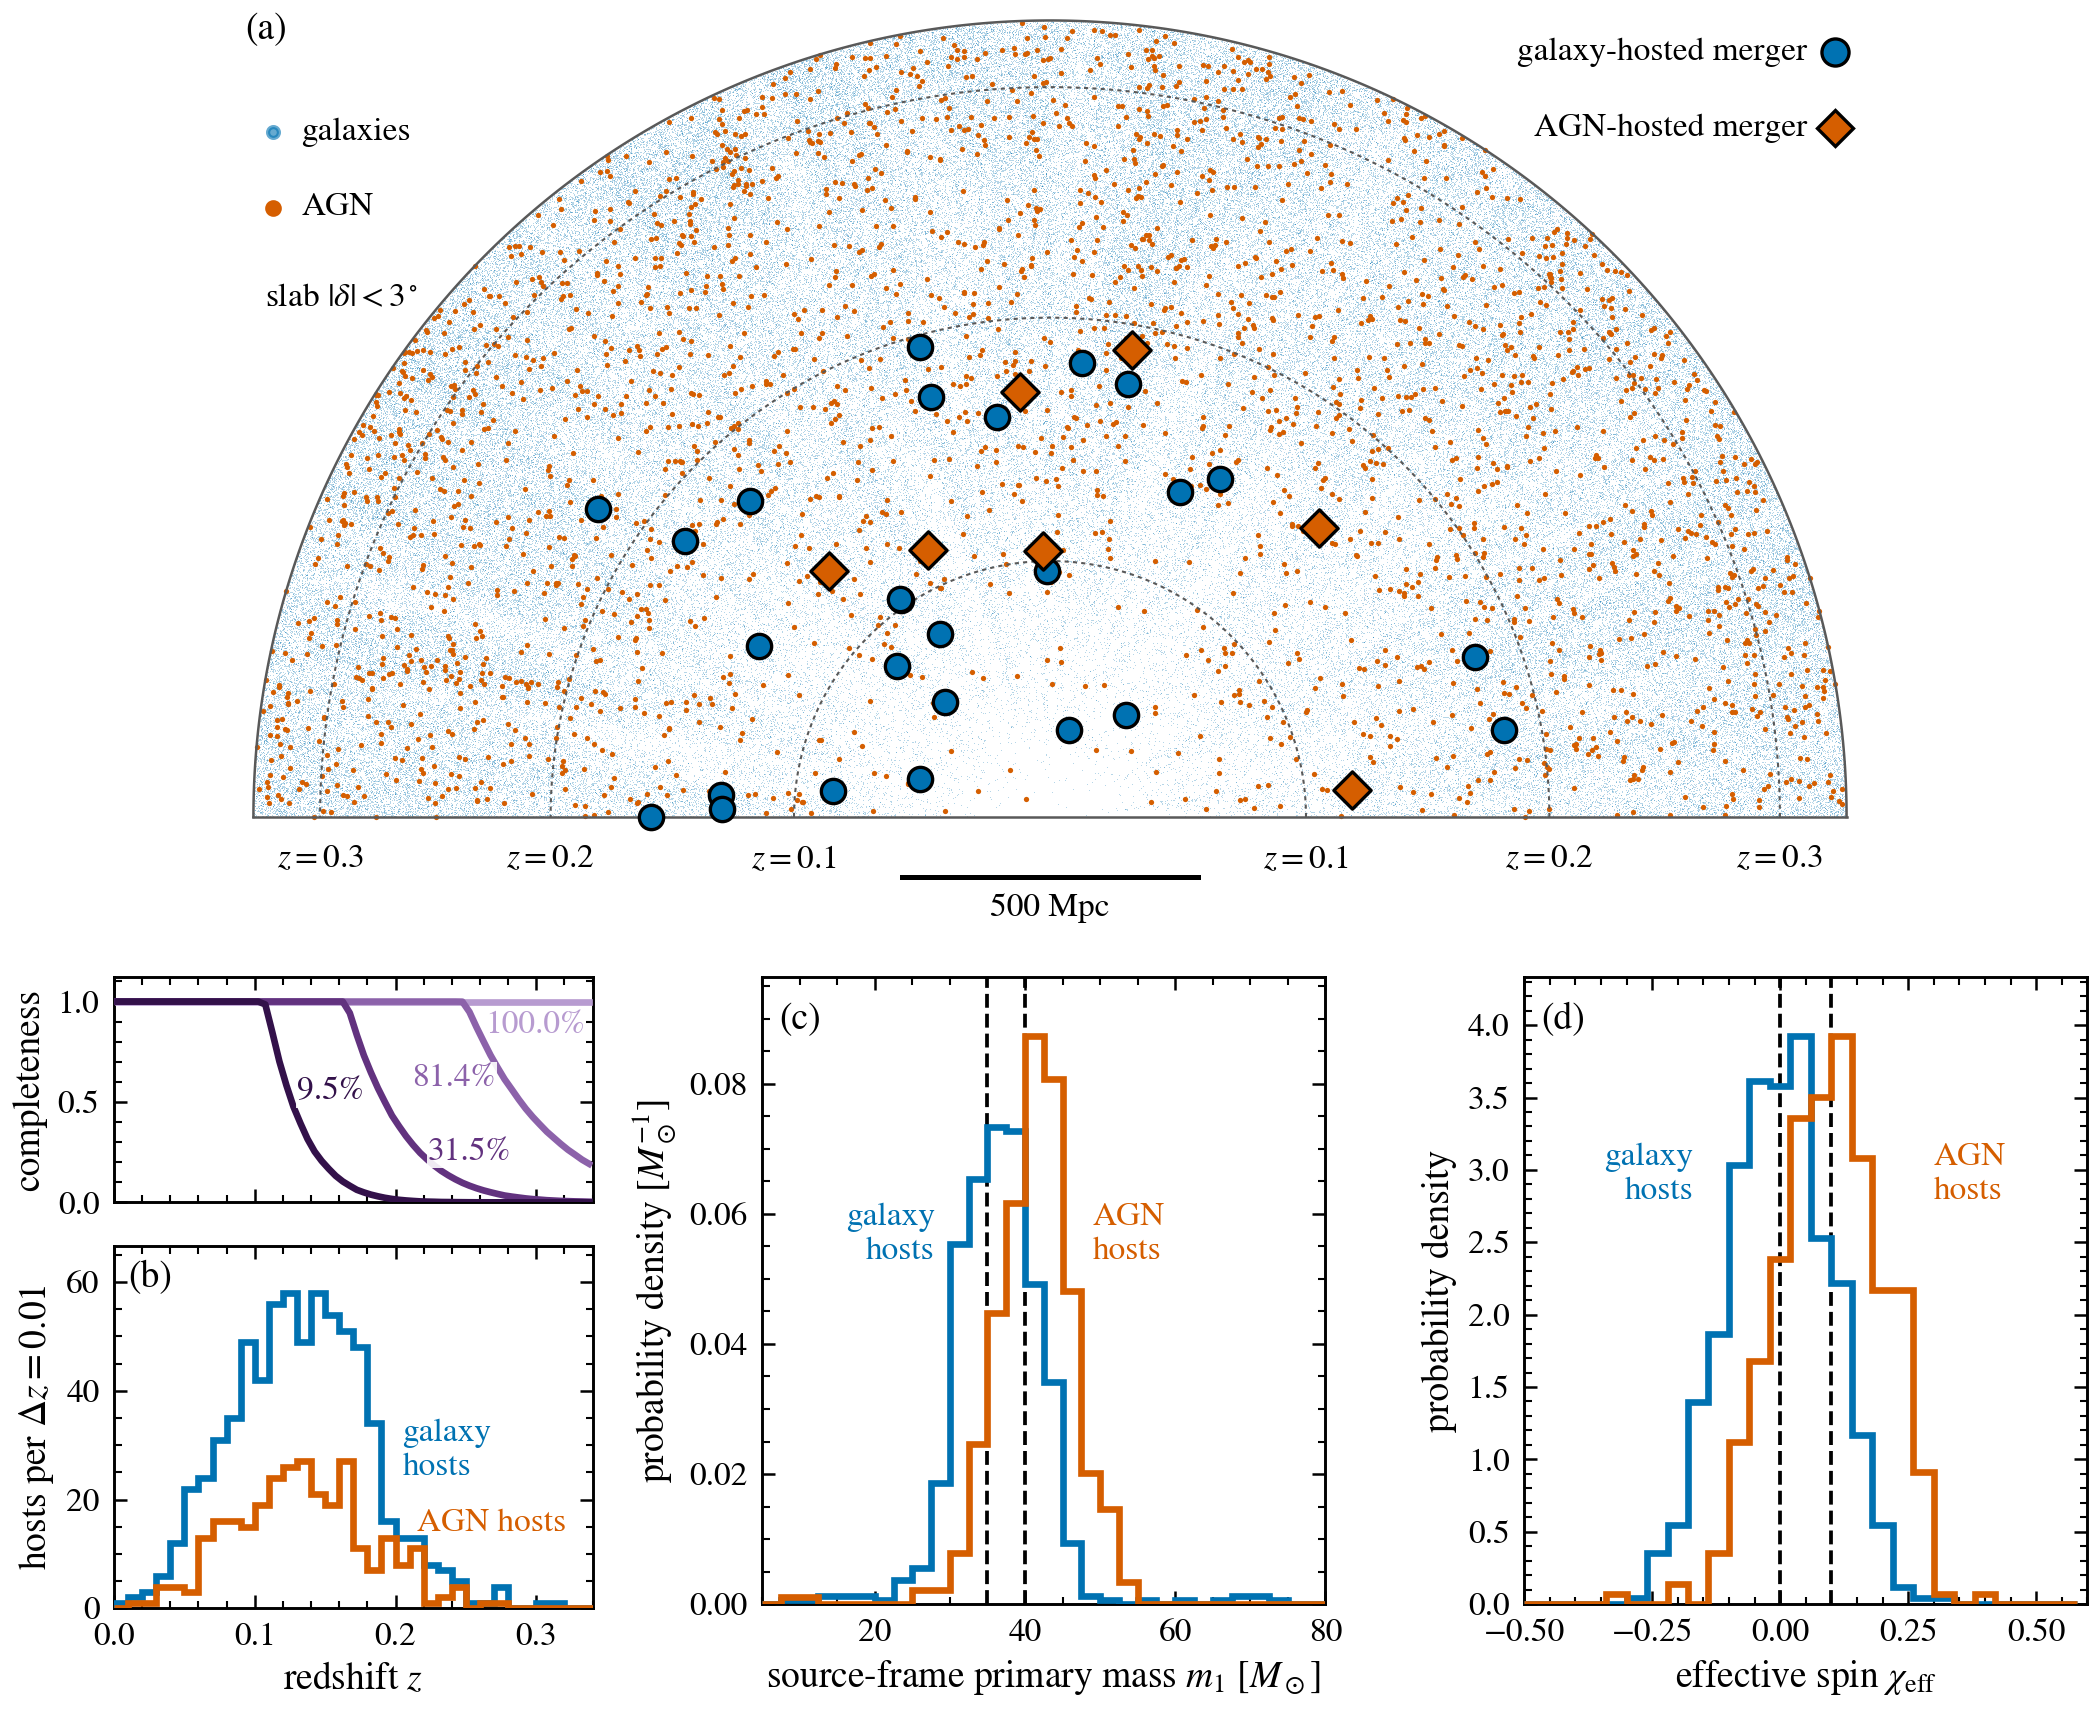
\includegraphics[width=\textwidth]{fig1_mocks}
\caption{The simulated catalogs. (a) A slab of declination
$|\delta|<3^\circ$ through one pair of catalogs, in comoving distance:
galaxies, AGN, and the hosts of the detected mergers that lie in it
(galaxy-hosted merger, AGN-hosted merger); dashed arcs are lines of constant
redshift. (b) Top: completeness of the catalogs against redshift for the
four flux limits, labeled with the completeness inside the horizon; bottom:
redshifts of the galaxy hosts and AGN hosts of the \MockNev{} detected
mergers. (c) Source-frame primary mass and (d) effective spin of the detected
mergers of the host-dependent mock, each host class normalized to unit area;
black dashed lines are the input peak locations and spin means. \prelim}
\label{fig:mocks}
\end{figure*}

\subsection{Galaxies and AGN}
\label{sec:cats}

The matter density is a lognormal field on concentric shells
$\MockShellWidth\,{\rm Mpc}$ thick out to $z=\MockzCat$, generated with
\textsc{glass} \cite{Tessore:2023zyk} from nonlinear matter power spectra
computed with \textsc{camb} \cite{Lewis:1999bs} in the cosmology of
Sec.~\ref{sec:intro}. Galaxies and AGN are Poisson samples of this one field,
each with a linear bias and a constant comoving number density.

The galaxies have a bias of \MockbGal{} and a number density
$\ngal=\MocknGal\,{\rm Mpc^{-3}}$. In the $B$-band Schechter function of
Ref.~\cite{Gehrels:2015uga}, which the GLADE catalog adopts
\cite{Dalya:2018cnd}, this is the density of galaxies brighter than
$\MockLcut\,L_\ast$, or $M_B<\MockMBcut$, the bright end of the galaxy
population. There are $\MockNGal$ of them out to $z=\MockzCat$.

The AGN have a bias of \MockbAGN{} and a number density
$\nagn=\MocknAGN\,{\rm Mpc^{-3}}$, a hundred times below the galaxies, which
gives $\MockNAGN$ objects. Both numbers are design choices, and the AGN class
is defined by them alone. The density is of the order of the
$10^{-4.75}\,{\rm Mpc^{-3}}$ adopted for luminous AGN in the association
studies \cite{Veronesi:2022hql,Bom:2023zgw}. Local AGN selected in hard
X-rays live in galaxy groups \cite{Powell:2018}; the bias of \MockbAGN,
against \MockbGal{} for the galaxies, makes the AGN the more strongly
clustered class, and we have not separated how much of what follows is owed
to the number density and how much to the bias. An input $\fagn$ of \MockfAGN{} lies below the current upper
limits on the fraction of mergers hosted by unobscured AGN, 0.41 to 0.61 at
95\% credibility \cite{Pouw:2026lar}, and those limits do not apply to
obscured AGN.

Every object carries a luminosity drawn from the same Schechter function
above the cut, and the apparent magnitude that follows at its redshift. An
AGN is given the apparent magnitude of a host galaxy drawn in this way, so
that one flux limit thins both catalogs with the same completeness
(Sec.~\ref{sec:fluxcats}). The AGN are drawn as a population of their own and
not as a subset of the galaxies; as a subset they would be one galaxy in a
hundred.

The cataloged redshift of every object is its true redshift with a Gaussian
error of $\sigma_z=\MockDz\,(1+z)$, and the kernel of Eq.~(\ref{eq:hosts})
has this width. The catalogs are therefore spectroscopic in quality. AGN
redshift errors stop limiting $\fagn$ once they fall below about 0.01
\cite{Pouw:2026lar}, so photometric AGN catalogs would return less than what
we find here.

\subsection{Mergers and their measurement}
\label{sec:events}

Each merger takes an AGN as its host with probability $\fagn=\MockfAGN$ and a
galaxy otherwise, chosen uniformly within the class and with a weight
$(1+z)^{-1}$ that keeps the merger rate per host constant in source-frame
time. The primary mass follows a power law of index $-\MockAlpha$ between
\MockMmin{} and $\MockMmax\msun$ with a Gaussian peak at $\mu_{\rm
G}=\MockMuG\msun$ of width $\sigma_{\rm G}=\MockSigmaG\msun$ that holds a
fraction \MockPeakFrac{} of the mergers \cite{Talbot:2018cva}. The mass ratio
follows $q^{\beta}$ with $\beta=\MockBeta$, and the effective spin a Gaussian
of mean $\mu_\chi=\MockMuChi$ and width $\sigma_\chi=\MockSigmaChi$. None of
these evolves with redshift.

The measurement is adapted from the model of Ref.~\cite{Farah:2023vsc}. The
signal
has an optimal signal-to-noise ratio $\rho$ that grows with the redshifted
chirp mass and falls as the inverse of the luminosity distance, with no
dependence on orientation. The observed value $\rho_{\rm obs}$ is $\rho$ plus
Gaussian noise of unit variance, and a merger is detected when $\rho_{\rm
obs}\geq\MockSNRthr$. The logarithms of the redshifted chirp mass and of the
mass ratio and the effective spin are measured with Gaussian errors of
\MockSigLnMc, \MockSigLnq{} and \MockSigChi{} times $\MockSNRthr/\rho_{\rm
obs}$, and the sky position with an error inversely proportional to
$\rho_{\rm obs}$, between $\MockSkyMin^\circ$ and $\MockSkyMax^\circ$ for the
detected events of the reference catalog. Without an orientation, $\rho_{\rm
obs}$ and the chirp mass together are the distance measurement, with a median
uncertainty of \MockSigLnDL\%. The posterior of an event is the exact
posterior of these data for a prior that is flat in the measured
quantities (Appendix~\ref{app:pe}).

Equation~(\ref{eq:like}) is the probability of the detected data, and the
mock respects that in two ways. Detection is decided by the observed
signal-to-noise ratio, the number on which the posterior is conditioned
\cite{Essick:2023upv}, and every measurement error is a function of observed
quantities, so the posterior of an event is exact for the data that selected
it.

Mergers are drawn until \MockNev{} are detected. In the reference catalog,
catalog A, the most distant detected merger is at $z=\MockzHorizon$, which we
call the horizon, the median redshift is \MockzMedian, and AGN host a
fraction \MockfAGNRealised{} of the detected mergers. We use \JointNcat{}
such catalogs, A to I, each with its own density field and with horizons from
\MockzHorizonMin{} to \MockzHorizonMax. For \PureNcat{} catalogs we also
draw one set of \MockNev{} mergers that are all hosted by galaxies and one
set that are all hosted by AGN. All of these mergers are closer and better
localized than most detections to date, and the precision reached here is
not a forecast.

\subsection{Host-dependent populations}
\label{sec:hdmock}

In the host-dependent mock the AGN-hosted mergers have their mass peak at
$\MockMuGAGN\msun$, an offset of $\dmuG=\MockDmuG\msun$, and a mean effective
spin offset by $\dmuchi=\MockDmuChi$; everything else is as for the galaxy
class [Fig.~\ref{fig:mocks}(c) and (d)]. The signs are those expected of
mergers in disks, where orbital alignment and repeated mergers favor heavier
black holes \cite{Yang:2019okq,Yang:2019cbr} and gas torques align the spins
\cite{McKernan:2021nwk,Li:2025iux}. The sizes are design choices. Each offset
equals the width of the distribution it shifts, so the two classes overlap
and no single event can be assigned to a class by its mass or its spin.

Heavier mergers are louder. AGN therefore host \MockHDNagn{} of the
\MockNev{} detected mergers of this mock, a fraction \MockHDfDet{} for an
input of \MockfAGN, and the detected fraction in Eq.~(\ref{eq:like}) is what
accounts for the difference.

Two further mocks separate masses, spins and positions. In the first the
AGN-hosted mergers differ in the spin mean only, by the same offset. In the
second every host is a galaxy and a fraction \MockCtrlBranchFrac{} of the
mergers, chosen without regard to the host, has the heavier and
faster-spinning population, so that no catalog can tell the two populations
apart. All three use the density field and the catalogs of catalog A, and
each is one simulated catalog.

\subsection{Flux-limited catalogs}
\label{sec:fluxcats}

Apparent-magnitude limits of $m<\MockMlimTwentyOne$, \MockMlimTwenty,
\MockMlimNineteen{} and \MockMlimEighteen, the same in every direction, leave
\MockCompTwentyOne\%, \MockCompTwenty\%, \MockCompNineteen\% and
\MockCompEighteen\% of the galaxies inside the horizon in the catalog, and
nearly the same fractions of the AGN [Fig.~\ref{fig:mocks}(b)]. We refer to
a limit by this completeness inside the horizon.

A flux limit removes the far hosts first. The shallowest catalog is complete
below $z=\MockzCompleteEighteen$ and loses its hosts steeply beyond, while
the median detected merger is at $z=\MockzMedian$. Its completeness of
\MockCompEighteen\% counts hosts, most of which lie near the horizon where
the volume is large and the detected mergers few: \MockEventFracCompleteEighteen\%
of the detected mergers lie where even this catalog is complete, and the
completeness weighted by the detected mergers is \MockEventCompEighteen\%.

In the analysis $C_k(z)$ is the fraction of the Schechter function brighter
than the limit at redshift $z$, with its parameters held at values fitted to
the catalogs, and the uncataloged hosts enter Eq.~(\ref{eq:hosts}) with the
number densities $n_k$. We take these densities at their inputs, assume an
AGN density that is off by factors between \DensityFactorLo{} and
\DensityFactorHi, or infer both. The merger catalog is that of catalog A at every limit; catalogs
B and C add two more at the shallowest.

%% ==========================================================================
\section{Results}
\label{sec:results}

\subsection{Two catalogs, one density field}
\label{sec:two}

With complete catalogs and a common population, $H_0$ and $\fagn$ are
recovered together and are nearly uncorrelated (Fig.~\ref{fig:two},
Table~\ref{tab:two}). The combined posterior of the \JointNcat{} catalogs
gives $H_0=\JointHzeroComb\,\kms$, which contains the input \MockHzero{} at
the \JointHzeroCombLevel\% credible level, and $\fagn=\JointfComb$, which
contains the input \MockfAGN{} at the \JointfCombLevel\% level; in the plane
of the two, the input lies on the boundary of the \JointCombLevelTwoD\%
highest-density region. The correlation coefficient of $H_0$ and $\fagn$ is
$\JointRhoComb$ in the combined posterior and between $\JointRhoMin$ and
$\JointRhoMax$ in single catalogs. We argue that the correlation is weak because the two
parameters act differently on the likelihood: $\fagn$ moves probability
between the galaxies and the AGN that share a localization volume, and $H_0$
slides the redshift scale of both catalogs together. Cross-Parkin \textit{et al.}~\cite{Cross-Parkin:2026pua}
found ``only a weak correlation'' between $H_0$ and the mixing fraction of
two weightings of one galaxy catalog, and we find the same for two distinct
catalogs whose number densities differ by a factor of a hundred. Among the
single catalogs, the input $H_0$ lies outside the 90\% interval of catalog D
and the input $\fagn$ outside that of catalog I.

\begin{figure*}
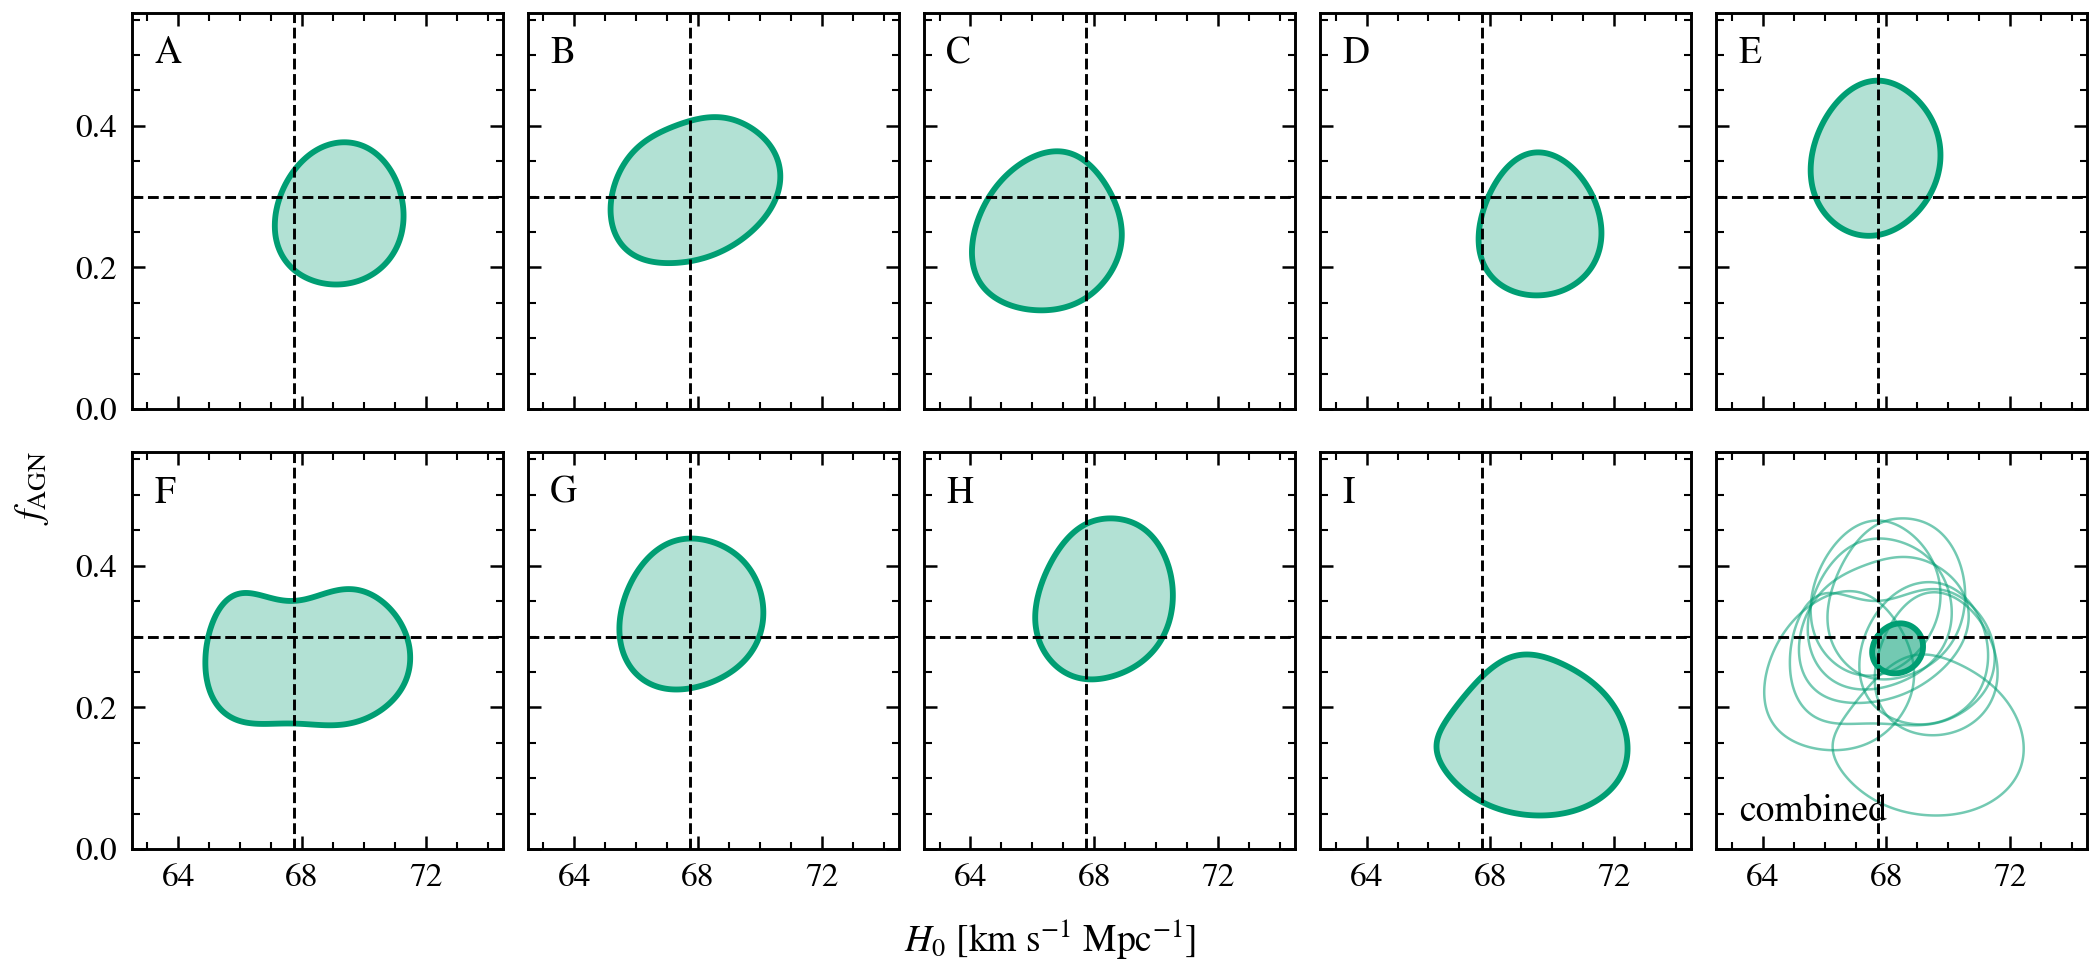
\includegraphics[width=\textwidth]{fig2_two_catalogs}
\caption{Joint posterior of $H_0$ and $\fagn$ from complete galaxy and AGN
catalogs with a common population. Panels A to I show the 90\%
highest-density region for each of \JointNcat{} simulated catalogs; the last
panel shows those regions as outlines and the 90\% region of the combined
posterior, filled. Black dashed lines are the input values. \prelim}
\label{fig:two}
\end{figure*}

\begin{table*}
\caption{Complete catalogs and a common population: posteriors of $H_0$ and
$\fagn$ from both catalogs, their correlation coefficient $\rho$, the Bayes
factor of two host classes against galaxy hosts only (Savage--Dickey ratio at
$\fagn=0$, prior U$[0,1]$), and $H_0$ from the galaxy catalog alone. Medians
and 90\% intervals; the inputs are $H_0=\MockHzero\,\kms$ and
$\fagn=\MockfAGN$.}
\label{tab:two}
\begin{ruledtabular}
\begin{tabular}{lccccc}
Catalog & $H_0$ [$\kms$] & $\fagn$ & $\rho$ & $\lB$ & $H_0$, galaxy catalog alone [$\kms$]\\
\hline
A & $\JointHzeroCatA$ & $\JointfCatA$ & $\JointRhoCatA$ & $\LBfZeroCatA$ & $\GalOnlyHzeroCatA$\\
B & $\JointHzeroCatB$ & $\JointfCatB$ & $\JointRhoCatB$ & $\LBfZeroCatB$ & $\GalOnlyHzeroCatB$\\
C & $\JointHzeroCatC$ & $\JointfCatC$ & $\JointRhoCatC$ & $\LBfZeroCatC$ & $\GalOnlyHzeroCatC$\\
D & $\JointHzeroCatD$ & $\JointfCatD$ & $\JointRhoCatD$ & $\LBfZeroCatD$ & $\GalOnlyHzeroCatD$\\
E & $\JointHzeroCatE$ & $\JointfCatE$ & $\JointRhoCatE$ & $\LBfZeroCatE$ & $\GalOnlyHzeroCatE$\\
F & $\JointHzeroCatF$ & $\JointfCatF$ & $\JointRhoCatF$ & $\LBfZeroCatF$ & $\GalOnlyHzeroCatF$\\
G & $\JointHzeroCatG$ & $\JointfCatG$ & $\JointRhoCatG$ & $\LBfZeroCatG$ & $\GalOnlyHzeroCatG$\\
H & $\JointHzeroCatH$ & $\JointfCatH$ & $\JointRhoCatH$ & $\LBfZeroCatH$ & $\GalOnlyHzeroCatH$\\
I & $\JointHzeroCatI$ & $\JointfCatI$ & $\JointRhoCatI$ & $\LBfZeroCatI$ & $\GalOnlyHzeroCatI$\\
\hline
Combined & $\JointHzeroComb$ & $\JointfComb$ & $\JointRhoComb$ & $\LBfZeroComb$ & $\GalOnlyHzeroComb$\\
\end{tabular}
\end{ruledtabular}
\end{table*}

Galaxy hosts alone cannot describe the mixed population, and yet $H_0$
hardly notices. The Bayes factor of two host classes against galaxy hosts
only is $\lB=\LBfZeroMin$ to \LBfZeroMax{} per catalog and \LBfZeroComb{}
for the \JointNcat{} combined, for a prior uniform on $[0,1]$ in $\fagn$.
The same events analyzed with the galaxy catalog alone give a combined
$H_0=\GalOnlyHzeroComb\,\kms$, with the input at the
\GalOnlyHzeroCombLevel\% credible level and a median
\ShiftGalOnlyMinusJointComb$\,\kms$ above that from both catalogs, a shift
smaller than its own interval [Fig.~\ref{fig:info}(b)]. We read this as a
consequence of the shared density field: the galaxy catalog still shows
where the AGN-hosted mergers are, because the AGN sit in the same structure.
This is the AGN case of the host-weighting systematic
\cite{Hanselman:2024hqy,Perna:2024lod,Alfradique:2025tbj}, and it agrees
with the findings that $H_0$ is stable against a wrong host weighting
\cite{Borghi:2025pav} and that physical weights add little once the catalog
is clustered \cite{Kalomenopoulos:2025qpt}. The evidence, and not $H_0$, is
what reveals the second host class, as for luminosity weights
\cite{Li:2025hrh}. The converse does not hold. With the AGN catalog alone
the $H_0$ posterior has no interior maximum in the prior range for
\AgnOnlyNoInterior{} of the \JointNcat{} catalogs, and the Bayes factor of
two host classes against AGN hosts only is $\lB=\LBfOneComb$ for the
\JointNcat{} combined: a sparse catalog cannot stand in for the galaxies
that host most of the mergers.

\begin{figure*}
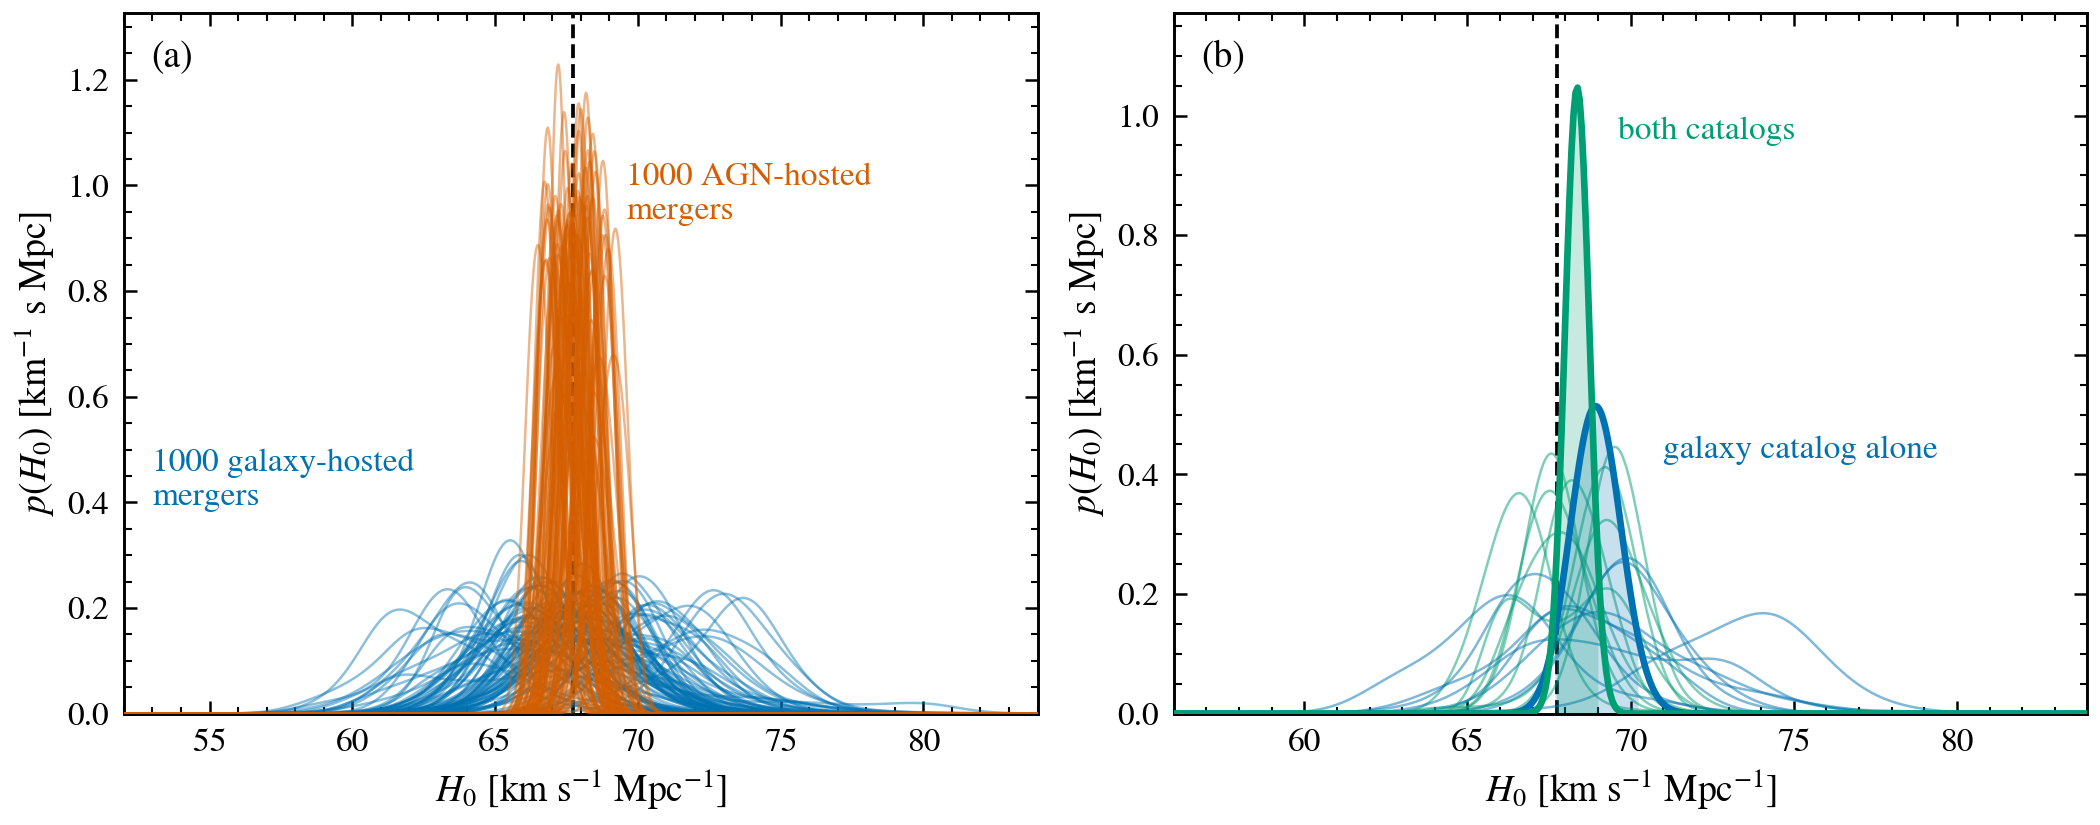
\includegraphics[width=\textwidth]{fig3_host_information}
\caption{Which hosts carry the information on $H_0$. (a) Posterior density
of $H_0$ for each of \PureNcat{} simulated catalogs with \MockNev{}
galaxy-hosted mergers, analyzed with the galaxy catalog (blue), and with
\MockNev{} AGN-hosted mergers, analyzed with the AGN catalog (vermilion).
(b) $H_0$ from all events of the catalogs of Fig.~\ref{fig:two} with the
galaxy catalog alone (blue) and with both catalogs (green); thin curves are
single catalogs and thick curves the combined posteriors, with their 90\%
intervals shaded. The black dashed line is the input value. \prelim}
\label{fig:info}
\end{figure*}

At equal numbers of events, AGN-hosted mergers constrain $H_0$
\PureRatioNinety{} times more tightly than galaxy-hosted ones
[Fig.~\ref{fig:info}(a)]. Over \PureNcat{} catalogs the mean 90\% half-width
of $H_0$ is $\PureAGNHalfNinety\,\kms$ for \MockNev{} AGN-hosted mergers and
the AGN catalog, against $\PureGalHalfNinety\,\kms$ for \MockNev{}
galaxy-hosted mergers and the galaxy catalog. We read the gain as a matter
of the number of candidate hosts. A localization volume holds
\PureGalHostsPerVol{} galaxies and \PureAGNHostsPerVol{} AGN on average, and
the AGN are the more clustered, so the redshift distribution of AGN along a
line of sight is a few narrow spikes where that of the galaxies is nearly
smooth. The direction is known:
rare hosts are easier to associate
\cite{Bartos:2017ggb,Alves:2020wnl,Bom:2023zgw,Pouw:2026lar}, an AGN catalog
improves $H_0$ from 3.7\% to 3.2\% for extreme-mass-ratio inspirals
\cite{Zhu:2024qpp}, and catalogs of galaxy clusters do the same for BBHs
\cite{Beirnaert:2025wcx}. What we add is the size of the effect for two
classes on one density field at equal numbers of events. The gain belongs to
the mergers that AGN host, and an AGN catalog delivers it only for that
fraction of the mergers. The ratio rests on the widths of the AGN-hosted
posteriors, the quantity most exposed to the Monte Carlo error whose size
Appendix~\ref{app:like} gives.

\subsection{Host-dependent masses and spins}
\label{sec:hd}

If mergers in AGN are heavier, an analysis with one population is biased in
$H_0$, and the host catalogs do not protect it (Fig.~\ref{fig:hdh0},
Table~\ref{tab:hd}). On the host-dependent mock the common-population
analysis with both catalogs gives $H_0=\CommonHzero\,\kms$, an interval that
excludes the input \MockHzero{} and whose median lies
$\ShiftCommonMinusFix\,\kms$ above that of the host-dependent model on the
same events. The sign is that of a mass-scale error in a spectral siren
measurement
\cite{Farr:2019twy,Ezquiaga:2022zkx,Mastrogiovanni:2021wsd,Pierra:2023deu}.
The model expects the peak at $\MockMuG\msun$; the AGN-hosted mergers arrive
with redshifted masses that belong to a peak at $\MockMuGAGN\msun$; and the
model accounts for them with a larger redshift at the measured distance,
which is a larger $H_0$. A correlation between $H_0$ and the fraction of a
heavier formation channel has been reported without catalogs
\cite{Scarpa:2026piy}. Here the heavier population is also a different host
class. The fraction stays at $\fagn=\CommonfAGN$, which we read as the
positions setting it. The common population of this comparison has its mass and spin
parameters fixed at the galaxy-class inputs. A common population with free parameters can settle between the two classes,
and gives $H_0=\CommonFreeHzero\,\kms$; the host-dependent model with the
same freedom is preferred to it by $\lB=\LBHDVsCommonFree$, for the offset
priors of Table~\ref{tab:priors}.

\begin{figure*}
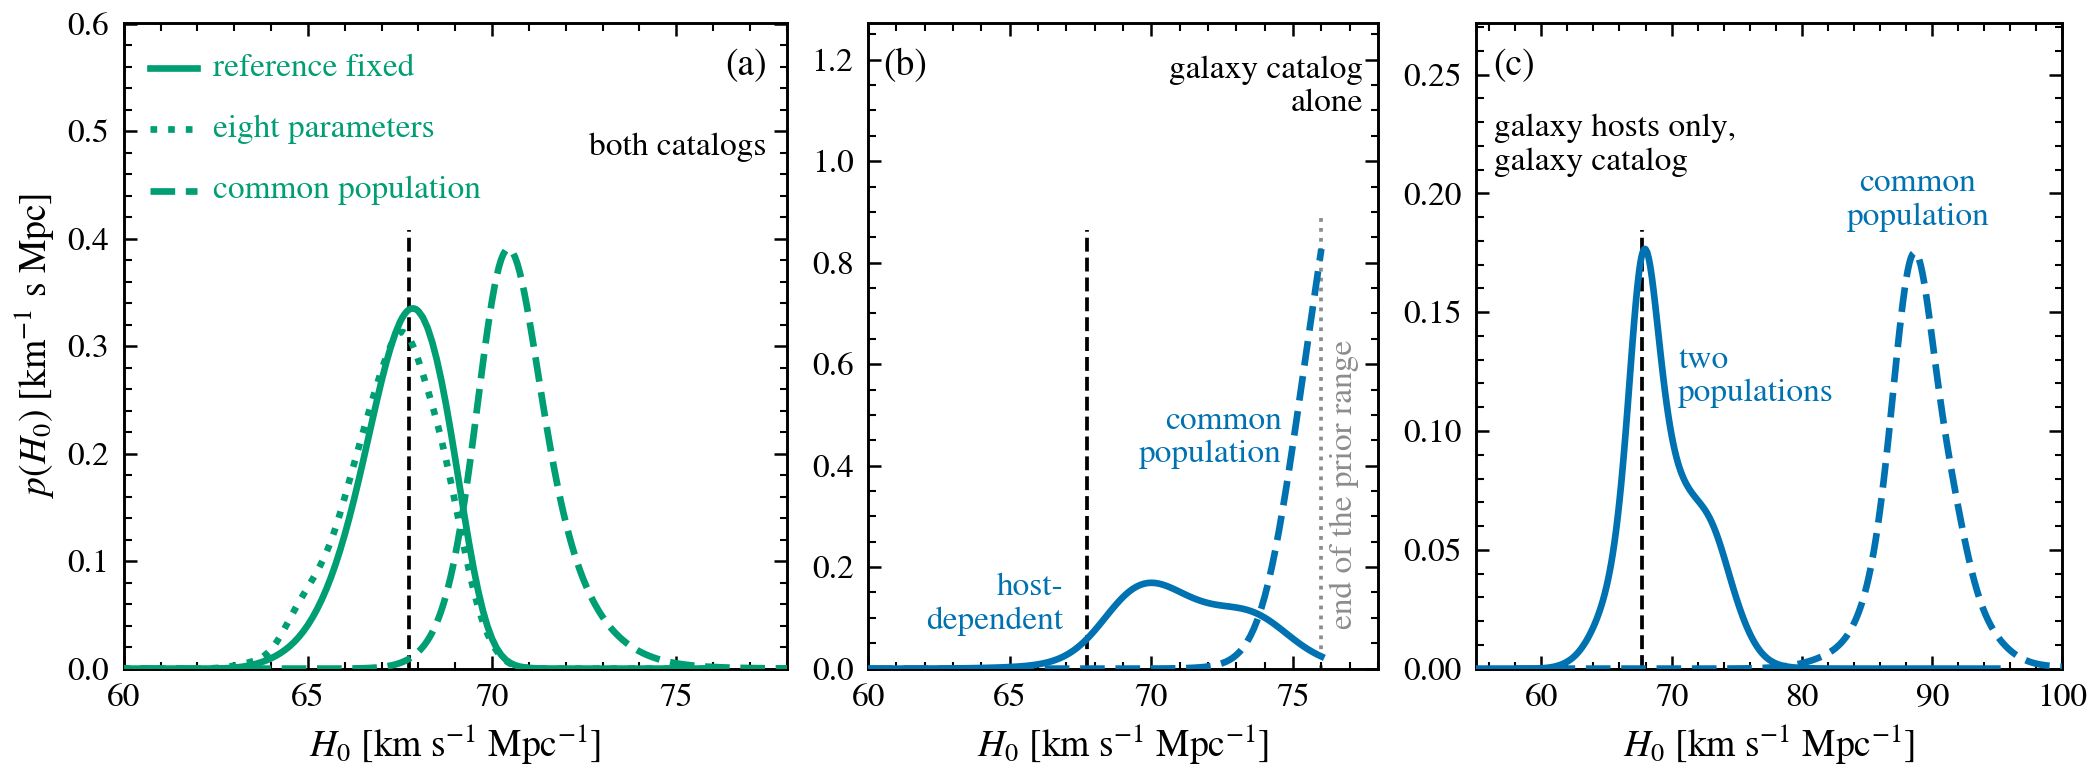
\includegraphics[width=\textwidth]{fig4_host_dependent_h0}
\caption{$H_0$ when AGN-hosted mergers are heavier and spin faster (one
simulated catalog in each panel); the black dashed line is the input value.
(a) Both catalogs: the host-dependent
model with the reference fixed (solid) and with eight parameters (dotted),
and the common population (dashed). (b) Galaxy catalog alone: the common
population (dashed), whose density is largest at the end of the prior range
(gray dotted line), and the host-dependent model with its offsets held fixed
(solid). (c) A mock with galaxy hosts only, galaxy catalog: the common
population (dashed) and two populations with the offsets held at their
inputs (solid). \prelim}
\label{fig:hdh0}
\end{figure*}

Less host information makes the bias larger. With the galaxy catalog alone
the common-population posterior has no interior maximum: its density is
largest at $\PriorHDHzeroHi\,\kms$, the upper end of the range
[Fig.~\ref{fig:hdh0}(b)]. In the mock where every host is a galaxy and no
catalog can separate the two populations, the common population gives
$H_0=\CtrlUnmodHzero\,\kms$ with its upper tail cut by the end of the prior
range, at least $\ShiftCtrlUnmodMinusMod\,\kms$ above the model with two
populations, which gives $\CtrlModHzero\,\kms$ with the input inside the
90\% interval and is preferred by $\lB=\LBCtrlModVsUnmod$
[Fig.~\ref{fig:hdh0}(c)]. We read the ordering as a competition between two
redshift scales. The catalogs tie the redshifts to the structure that the
events trace, and the more of that structure is resolved, the less the
misplaced mass scale can move $H_0$, in line with the correlation between
$H_0$ and the mass scale that grows as a catalog becomes incomplete
\cite{Borghi:2025pav}. Two catalogs leave $\ShiftCommonMinusFix\,\kms$ of
it.

Letting each host class have its own mass peak and spin mean recovers $H_0$,
$\fagn$ and both offsets (Fig.~\ref{fig:offsets}). With the reference
population fixed and the offsets free we find $H_0=\HDFixHzero\,\kms$,
$\fagn=\HDFixfAGN$, $\dmuG=\HDFixDmuG\msun$ for an input of \MockDmuG, and
$\dmuchi=\HDFixDmuChi$ for an input of \MockDmuChi; the four inputs lie
inside their 90\% intervals. The host-dependent model is preferred to the
common population by $\lB=\LBOffsetsVsCommon$, for priors uniform on
$[\PriorDmuGLo,\PriorDmuGHi]\msun$ in $\dmuG$ and on
$[\PriorDmuChiLo,\PriorDmuChiHiSix]$ in $\dmuchi$. Its $H_0$ interval is
\WRatioFixOverCommon{} times as wide as that of the common population. The
host-dependent model adds no precision in $H_0$. It removes the bias.

\begin{figure*}
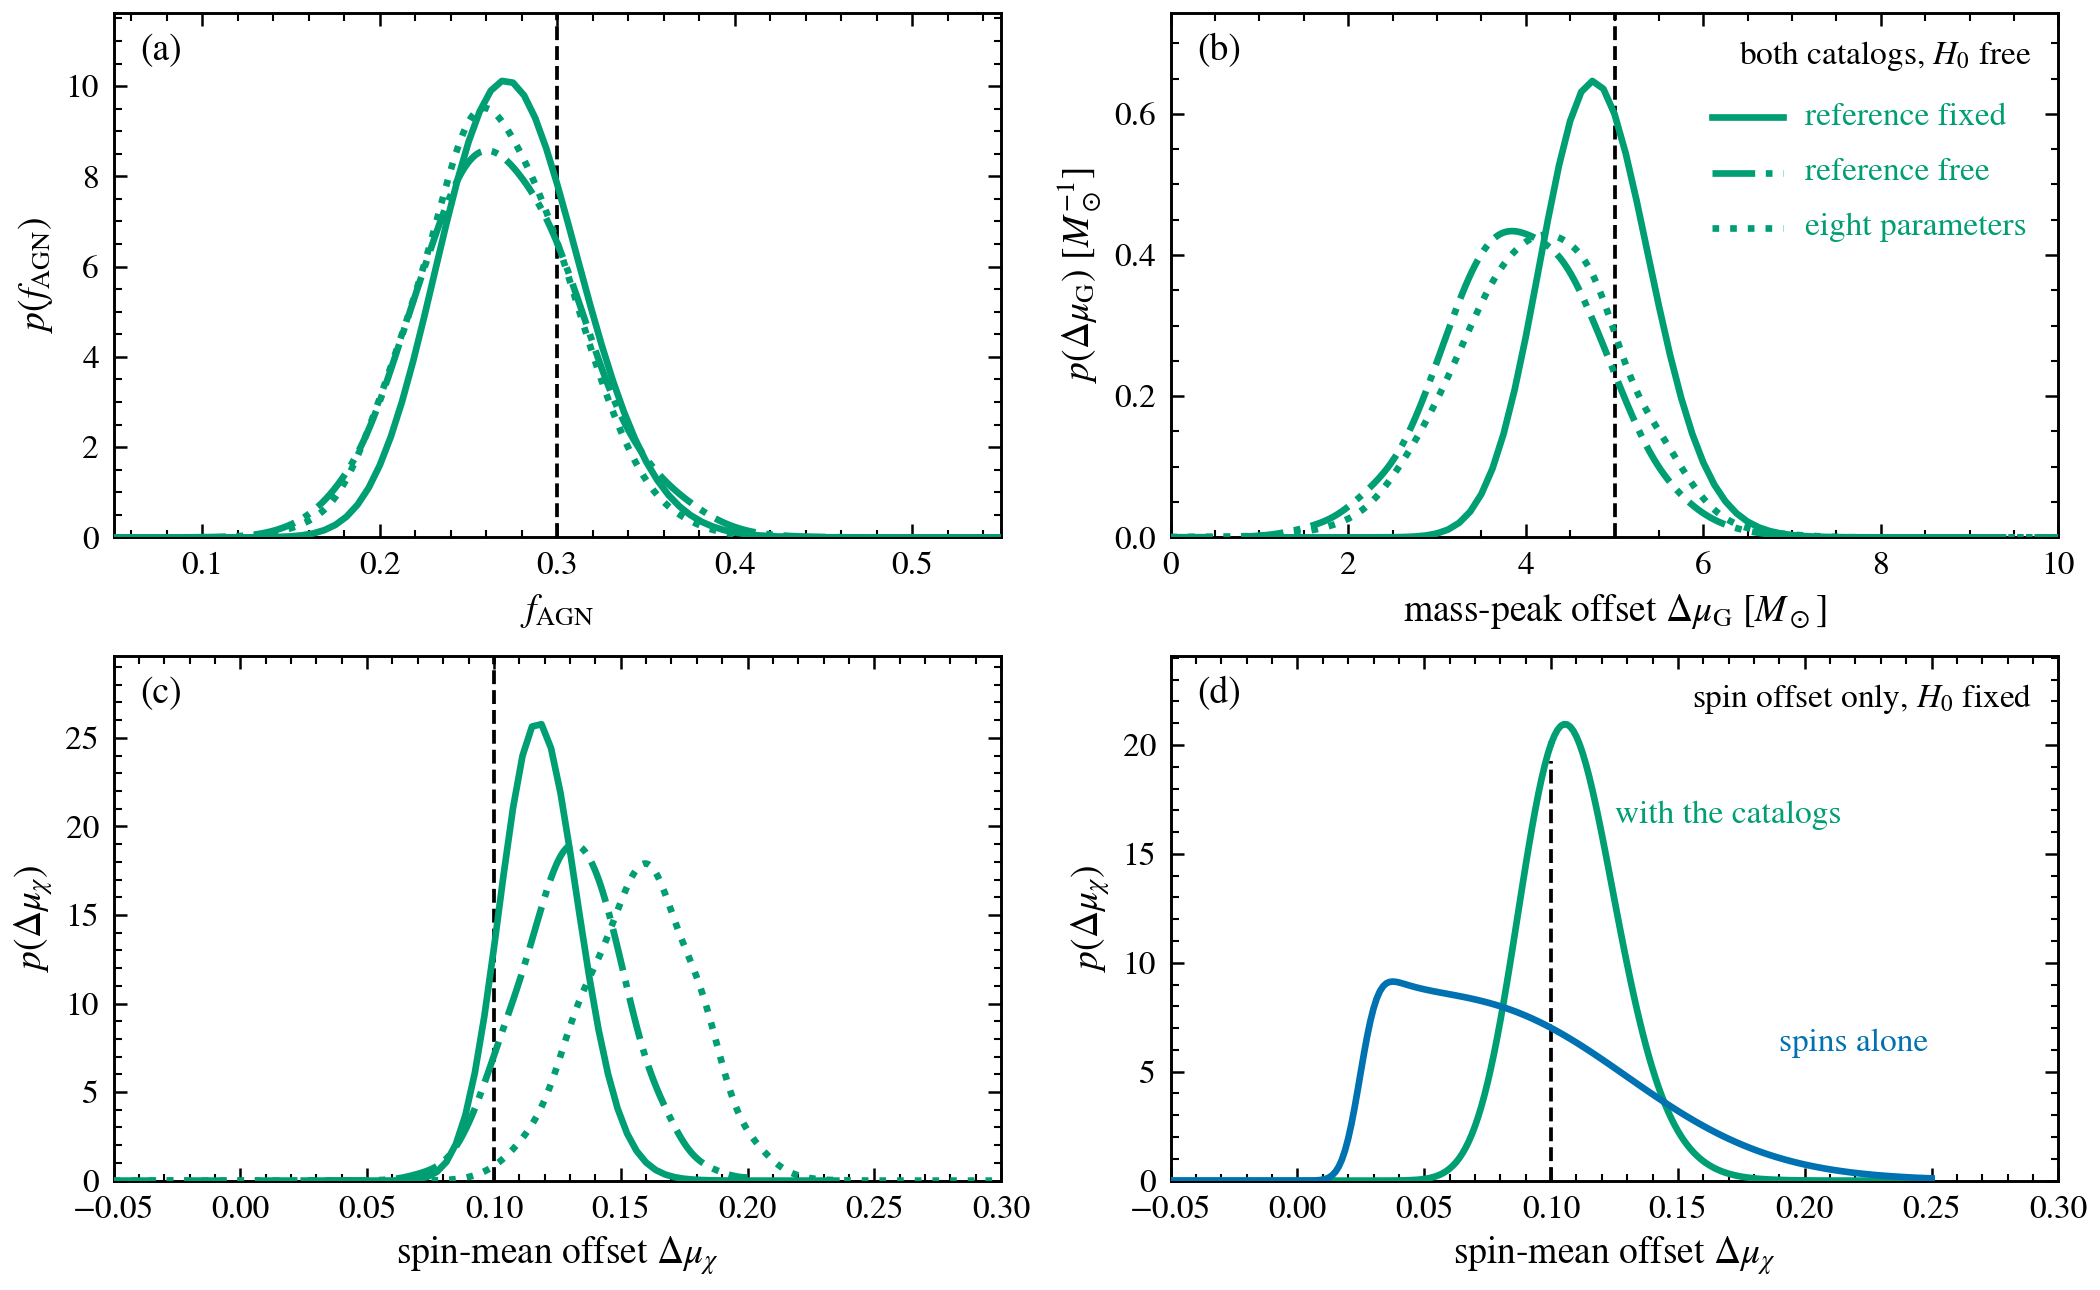
\includegraphics[width=\textwidth]{fig5_offsets}
\caption{Posteriors of (a) $\fagn$, (b) the mass-peak offset $\dmuG$ and (c)
the spin-mean offset $\dmuchi$ on the host-dependent mock with both catalogs
and $H_0$ free: reference fixed (solid), reference free (dash-dotted) and
eight parameters (dotted). (d) The spin-mean offset on the mock with a spin
offset only, at fixed $H_0$: with the catalogs (green) and from spins alone
(blue), which ends at the edge of its prior. Black dashed lines are the
input values. \prelim}
\label{fig:offsets}
\end{figure*}

\begin{table*}
\caption{Analyses of the mocks with host-dependent populations (one simulated
catalog each). $\lB$ compares each model with the common population on the
same events and catalogs. Offsets labeled ``fixed'' are held at the stated
values and not inferred. Medians and 90\% intervals.}
\label{tab:hd}
\begin{ruledtabular}
\begin{tabular}{lccccc}
Model & $H_0$ [$\kms$] & $\fagn$ & $\dmuG$ [$M_\odot$] & $\dmuchi$ & $\lB$\\
\hline
Input & \MockHzero & \MockfAGN & \MockDmuG & \MockDmuChi & \\
\hline
\multicolumn{6}{l}{Host-dependent mock, both catalogs}\\
Common population & $\CommonHzero$ & $\CommonfAGN$ & 0 & 0 & 0\\
Common population, free parameters & $\CommonFreeHzero$ & $\CommonFreefAGN$ & 0 & 0 & \\
Offsets free, reference fixed & $\HDFixHzero$ & $\HDFixfAGN$ & $\HDFixDmuG$ & $\HDFixDmuChi$ & $\LBOffsetsVsCommon$\\
Reference free (six parameters) & $\HDFreeHzero$ & $\HDFreefAGN$ & $\HDFreeDmuG$ & $\HDFreeDmuChi$ & $\LBFreeRefVsCommon$\\
Widths free (eight parameters) & $\HDEightHzero$ & $\HDEightfAGN$ & $\HDEightDmuG$ & $\HDEightDmuChi$ & $\LBEightVsCommon$\\
\hline
\multicolumn{6}{l}{Host-dependent mock, galaxy catalog alone}\\
Common population & \multicolumn{2}{l}{no interior maximum below $\PriorHDHzeroHi$} & 0 & 0 & \\
Offsets fixed & $\PinIOneHzero$ & & \PinDmuG, fixed & \PinDmuChi, fixed & \\
\hline
\multicolumn{6}{l}{Galaxy hosts only, galaxy catalog}\\
Common population & $\CtrlUnmodHzero$ & & 0 & 0 & 0\\
Two populations, offsets fixed & $\CtrlModHzero$ & $\CtrlModfBranch$ & \MockDmuG, fixed & \MockDmuChi, fixed & $\LBCtrlModVsUnmod$\\
\end{tabular}
\end{ruledtabular}
\end{table*}

Inferring the reference population as well leaves $H_0$ in place. With the
reference peak location and spin mean free we find $H_0=\HDFreeHzero\,\kms$,
and with the two widths free too, eight parameters in all,
$H_0=\HDEightHzero\,\kms$ and $\fagn=\HDEightfAGN$, with the inputs of $H_0$
and $\fagn$ inside these 90\% intervals (Appendix~\ref{app:corner}). The offsets are measured \WRatioFreeDmuGOverFix{} and
\WRatioFreeDmuChiOverFix{} times less tightly once the reference is free.
Freeing the reference is not rewarded, since the fixed one sits at its
input: the Bayes factor of the free reference against the fixed one is
$\lB=\LBFreeRefVsFix$, and that of the free widths against the fixed ones is
$\LBEightVsFree$, for the priors of Table~\ref{tab:priors}. $H_0$ follows the mass scale of the majority:
its correlation coefficient with $\mu_{\rm G}$ is $\HDEightRhoHzeroMuG$ and
with $\dmuG$ it is $\HDEightRhoHzeroDmuG$. Not every input is contained. In the
eight-parameter model the spin-mean offset is $\dmuchi=\HDEightDmuChi$, a
90\% interval that excludes the input \MockDmuChi, and the same holds for
$\mu_{\rm G}=\HDEightMuG\msun$ against \MockMuG{} and for
$\sigma_\chi=\HDEightSigmaChi$ against \MockSigmaChi. This is one simulated
catalog. Over \HDNcat{} catalogs combined, the inputs of $\dmuG$ and
$\dmuchi$ lie at the \HDEightDmuGCombLevel\% and \HDEightDmuChiCombLevel\%
credible levels (Sec.~\ref{sec:validation}).

Positions and intrinsic parameters both identify the host class, and they
help each other unequally [Fig.~\ref{fig:offsets}(d)]. On the mock with a
spin offset only, and with $H_0$ held at its input, the positions alone give
$\fagn=\SpinPosfAGN$ and modeling the spin offset gives $\SpinBothfAGN$: the
width of the 90\% interval changes by $\SpinfWidthChange\%$, so $\fagn$ is
set almost entirely by where the mergers are. The spin offset gains far more. We
find $\dmuchi=\SpinBothDmuChi$ with the catalogs and $\SpinIntDmuChi$ from
spins alone, a 90\% interval \SpinDmuChiWidthRatio{} times wider, and the
Bayes factor against no offset is $\lB=\LBSpinFixH$ with the catalogs and
\LBSpinIntFixH{} without, for a prior uniform on
$[\PriorSpinDmuChiLo,\PriorSpinDmuChiHi]$; the posterior from spins alone
reaches the upper end of that prior, so the factor of \SpinDmuChiWidthRatio{}
depends slightly on the range. The catalogs say which events are likely to be AGN-hosted, and the
spin distribution of that class can then be read off, where spins alone must
separate two overlapping Gaussians. This is the joint inference that the
disagreement between position-based and spin-based identifications of
candidate AGN mergers calls for \cite{Pouw:2026lar,Bartos:2026xlt}. We have
shown it for the spin, which is not redshifted and does not affect
detection. The mass is coupled to the position through detection, since the
heavier AGN-hosted mergers are overrepresented among the detected events
(Sec.~\ref{sec:hdmock}).

\subsection{Flux limits and the number of missing hosts}
\label{sec:flux}

Flux limits cost little precision when the number densities of the
uncataloged hosts are known [Fig.~\ref{fig:flux}(a) and (c),
Table~\ref{tab:flux}]. At \MockCompEighteen\% completeness we find
$H_0=\FluxHzeroEighteen\,\kms$ and $\fagn=\FluxfEighteen$ on catalog A, with
both inputs inside the 90\% intervals. These intervals are wider than those
from the complete catalogs by factors of \FluxHzeroRatioEighteen{} and
\FluxfRatioEighteen, and the $H_0$ median moves by
$\FluxHzeroShiftEighteen\,\kms$, against a 90\% half-width of
$\FluxHzeroHalfEighteen\,\kms$. We attribute the small cost to two things. The mergers are nearer than the hosts that the flux limit removes
(Sec.~\ref{sec:fluxcats}), and the uncataloged hosts enter
Eq.~(\ref{eq:hosts}) with their true number density, so the model dilutes
the cataloged structure by the right amount. For $H_0$ this is in line with
studies of catalog completeness
\cite{Gray:2019ksv,Borghi:2025pav,Kalomenopoulos:2025qpt,VanWyngarden:2025ogy}.
A completion that follows the large-scale structure does better than a
uniform one at low completeness
\cite{Dalang:2023ehp,Leyde:2025rzk,Barbieri:2026fdy,Tagliazucchi:2026qwy},
and ours is uniform. We are not aware of an earlier statement for $\fagn$.

\begin{figure*}
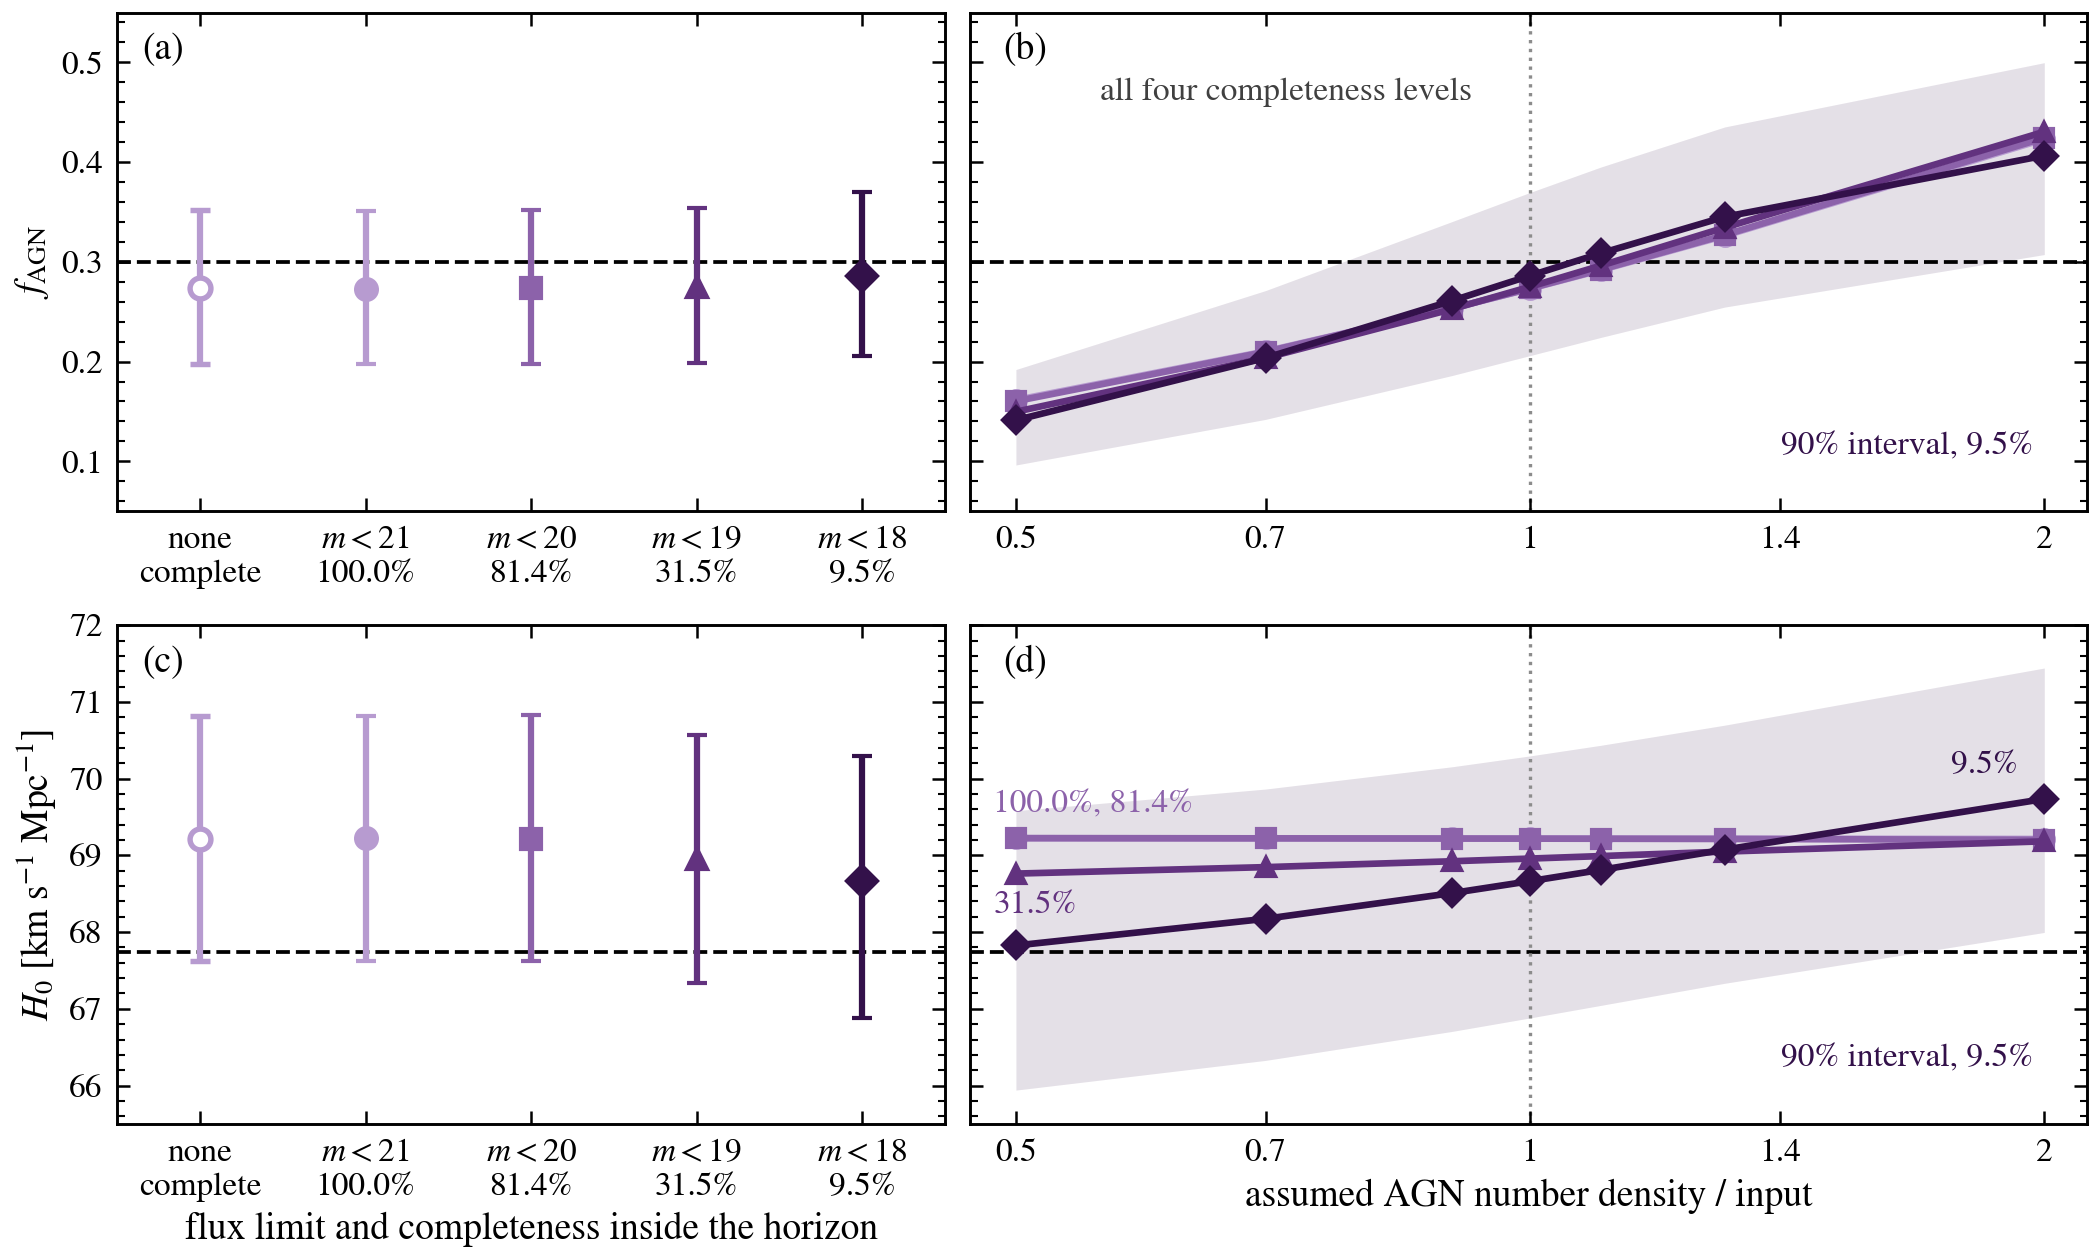
\includegraphics[width=\textwidth]{fig6_flux_limits}
\caption{Flux limits and the assumed AGN number density (one simulated
catalog). (a) $\fagn$ and (c) $H_0$, medians and 90\% intervals, against the
flux limit and completeness inside the horizon, with the number densities of
the uncataloged hosts at their inputs; the open circle is the complete
catalog. (b) and (d) Medians against the assumed AGN number density in units
of its input, one curve per flux limit with the symbols of (a); the band is
the 90\% interval at \MockCompEighteen\% completeness. Black dashed lines
are the input values. \prelim}
\label{fig:flux}
\end{figure*}

\begin{table*}
\caption{Flux-limited catalogs (catalog A). Completeness inside the horizon;
$H_0$ and $\fagn$ with the number densities of the uncataloged hosts at
their inputs; the change of the posterior medians per decade of the assumed
AGN number density; and the posteriors when both number densities are
inferred. The inputs are $\log_{10}(\ngal/{\rm Mpc^{-3}})=\MockLognGal$ and
$\log_{10}(\nagn/{\rm Mpc^{-3}})=\MockLognAGN$. Medians and 90\% intervals,
$H_0$ in $\kms$.}
\label{tab:flux}
\begin{ruledtabular}
\begin{tabular}{lccccccccc}
 & & \multicolumn{2}{c}{Densities at inputs} & \multicolumn{2}{c}{Per decade of $\nagn$} & \multicolumn{4}{c}{Densities inferred}\\
Limit & Compl. & $H_0$ & $\fagn$ & $d\fagn$ & $dH_0$ & $\log_{10}\ngal$ & $\log_{10}\nagn$ & $\fagn$ & $H_0$\\
\hline
none & complete & $\JointHzeroCatA$ & $\JointfCatA$ & & & & & & \\
$m<\MockMlimTwentyOne$ & \MockCompTwentyOne\% & $\FluxHzeroTwentyOne$ & $\FluxfTwentyOne$ & $\SlopefAGNTwentyOne$ & $\SlopeHzeroTwentyOne$ & $\FreeLognGalTwentyOne$ & $\FreeLognAGNTwentyOne$ & $\FreefAGNTwentyOne$ & $\FreeHzeroTwentyOne$\\
$m<\MockMlimTwenty$ & \MockCompTwenty\% & $\FluxHzeroTwenty$ & $\FluxfTwenty$ & $\SlopefAGNTwenty$ & $\SlopeHzeroTwenty$ & $\FreeLognGalTwenty$ & $\FreeLognAGNTwenty$ & $\FreefAGNTwenty$ & $\FreeHzeroTwenty$\\
$m<\MockMlimNineteen$ & \MockCompNineteen\% & $\FluxHzeroNineteen$ & $\FluxfNineteen$ & $\SlopefAGNNineteen$ & $\SlopeHzeroNineteen$ & $\FreeLognGalNineteen$ & $\FreeLognAGNNineteen$ & $\FreefAGNNineteen$ & $\FreeHzeroNineteen$\\
$m<\MockMlimEighteen$ & \MockCompEighteen\% & $\FluxHzeroEighteen$ & $\FluxfEighteen$ & $\SlopefAGNEighteen$ & $\SlopeHzeroEighteen$ & $\FreeLognGalEighteen$ & $\FreeLognAGNEighteen$ & $\FreefAGNEighteen$ & $\FreeHzeroEighteen$\\
\end{tabular}
\end{ruledtabular}
\end{table*}

What the mergers measure is the merger rate per host, and $\fagn$ follows
only after the uncataloged hosts are counted. Wherever no event has weight
in the incomplete part of a catalog, the events and the detected fraction
see only the first term of Eq.~(\ref{eq:hosts}), which we write $c_k/Z_k$.
The mixture of Eq.~(\ref{eq:mixture}) is then proportional to
$(1-\tilde f)\,c_{\rm gal}/N_{\rm gal}+\tilde f\,c_{\rm AGN}/N_{\rm AGN}$,
with
\begin{equation}
\ln\frac{\tilde f}{1-\tilde f}=\ln\frac{\fagn}{1-\fagn}
+\ln\frac{F_{\rm AGN}}{F_{\rm gal}} .
\label{eq:identity}
\end{equation}
The factor of proportionality is the same in every event and in the
detected fraction and cancels in Eq.~(\ref{eq:like}). The likelihood
therefore depends on $\fagn$, $\ngal$ and $\nagn$ only through $\tilde f$.

In physical terms $\tilde f$ is the fraction of mergers hosted by AGN among
the mergers in cataloged hosts, and the mergers measure the merger rate per
cataloged AGN, $r_{\rm AGN}$, relative to the merger rate per cataloged
galaxy, $r_{\rm gal}$. The catalogs show which objects are AGN and which are
galaxies, and the mergers answer with how many more mergers one hosts than
the other. The odds that a merger is hosted by an AGN are that ratio times the
ratio of the numbers of hosts,
\begin{equation}
\frac{\fagn}{1-\fagn}=\frac{r_{\rm AGN}}{r_{\rm gal}}\,
\frac{Z_{\rm AGN}}{Z_{\rm gal}} ,
\label{eq:rates}
\end{equation}
and the numbers $Z_k$ of Eq.~(\ref{eq:norm}) count the hosts a catalog lacks
as well as those it holds. With the number densities at their inputs,
$F_{\rm AGN}=F_{\rm gal}$ and $\tilde f=\fagn$, which is why the posteriors
of Fig.~\ref{fig:flux}(a) do not move with the flux limit. For the same data,
Eqs.~(\ref{eq:norm}) and (\ref{eq:identity}) give
\begin{equation}
\frac{\partial}{\partial\ln\nagn}\ln\frac{\fagn}{1-\fagn}=1-F_{\rm AGN} .
\label{eq:slope}
\end{equation}

In the analyses here the host populations are normalized out to $z_{\rm
max}=\NormZmax$, far beyond the catalogs, which end at $z=\MockzCat$, and
the events, which end at $z=\MockzHorizon$. The cataloged share is then
$F_{\rm AGN}<\NormFAGNMax$ at every flux limit: almost all of $Z_{\rm AGN}$
is uncataloged hosts that no event can reach, and Eq.~(\ref{eq:slope}) is at
its limit of one. We find that $\fagn$ changes by \SlopefAGNMin{} to
\SlopefAGNMax{} per decade of the assumed AGN number density
[Fig.~\ref{fig:flux}(b)]. A factor of two in the density moves $\fagn$ by
\DeltafTwoTwentyOne, against a 90\% half-width of \FluxfHalfTwentyOne. At
the two deepest limits Eq.~(\ref{eq:identity}), applied to the posterior at
the input density, reproduces the change, \SlopefAGNIdentityTwentyOne{} and
\SlopefAGNIdentityTwenty{} per decade against \SlopefAGNTwentyOne{} and
\SlopefAGNTwenty; at the two shallowest the events that lie in the
incomplete part of the catalogs add to it. The change is the same at
every depth because the normalization volume is the same, not because
completeness is of no help. If the host populations are normalized over the
volume in which a catalog is complete, $F_{\rm AGN}=1$ and the assumed
density drops out of Eq.~(\ref{eq:slope}); for the normalization over the
depth of the catalogs we find \SlopefAGNDepthNorm{} per decade. The general
statement is Eq.~(\ref{eq:rates}): $\fagn$ refers to a volume, and it needs
the number of AGN in that volume.

$H_0$ is nearly untouched. The normalizations $Z_k$ change the relative
weight of the two host classes and not the redshift scale, so $H_0$ depends
on the assumed AGN density only through the events in the incomplete part of
the catalogs: by $\SlopeHzeroEighteen\,\kms$ per decade at
\MockCompEighteen\% completeness, which is $\DeltaHzeroTwoEighteen\,\kms$
for a factor of two, and by $\SlopeHzeroTwenty\,\kms$ per decade at
\MockCompTwenty\% [Fig.~\ref{fig:flux}(d)].

The degeneracy itself is known. In the likelihood of the association
searches $\fagn$ multiplies the completeness of the AGN catalog
\cite{Zhu:2025rdv}; Zhu \textit{et al.}~\cite{Zhu:2024qpp} name the
degeneracy between the two and the dependence on the AGN density;
Cross-Parkin \textit{et al.}~\cite{Cross-Parkin:2026pua} note that
incompleteness is ``potentially degenerate with the astrophysical weighting
of the host population''; Pouw \textit{et al.}~\cite{Pouw:2026lar} note that
their $\fagn$ depends on the maximum redshift of the merger populations,
which changes the two normalizations differently; and Bom and Palmese
\cite{Bom:2023zgw} find that a fixed AGN number density carries cosmological
information of its own. Equations~(\ref{eq:identity}) to
(\ref{eq:slope}) give its size and say which quantity survives it.

With both number densities free, the mergers bound the galaxy density and
leave the AGN density, and with it $\fagn$, to the prior
(Fig.~\ref{fig:free}). At \MockCompEighteen\% completeness we find
$\log_{10}(\ngal/{\rm Mpc^{-3}})=\FreeLognGalEighteen$ for an input of
$\MockLognGal$ on catalog A, and $\FreeLognGalEighteenCatB$ and
$\FreeLognGalEighteenCatC$ on catalogs B and C, with the input inside all
three 90\% intervals. The posterior has a sharp upper edge and a tail to the
lower end of the prior. We argue that the edge is set by the events beyond the
complete part of the catalog. There the uncataloged galaxies are spread
uniformly, and too large a density erases the clustering of the cataloged
galaxies, which the events follow; too small a density costs little. The AGN density
has the same term, but AGN host a minority of the mergers and
Eq.~(\ref{eq:rates}) lets $\fagn$ absorb their number. Its posterior,
$\log_{10}(\nagn/{\rm Mpc^{-3}})=\FreeLognAGNEighteen$ for an input of
$\MockLognAGN$, rises to \FreeLognAGNPeakOverPrior{} times the prior density
and no more, its correlation coefficient with $\fagn$ is
\FreeRhofAGNEighteen, and the 90\% interval of $\fagn$ covers
\FreefWidthEighteen{} of the prior range, against 0.90 for the prior itself.
The difference between the two classes is one of degree. $H_0$ is spared: we
find $\FreeHzeroEighteen\,\kms$, with medians that differ by
$\FreeHzeroSpread\,\kms$ across the four flux limits. Bom and Palmese
\cite{Bom:2023zgw} suggested that ``one would leave the AGN number density
free to vary''. Doing so costs $H_0$ little, and it costs $\fagn$ its
measurement.

\begin{figure*}
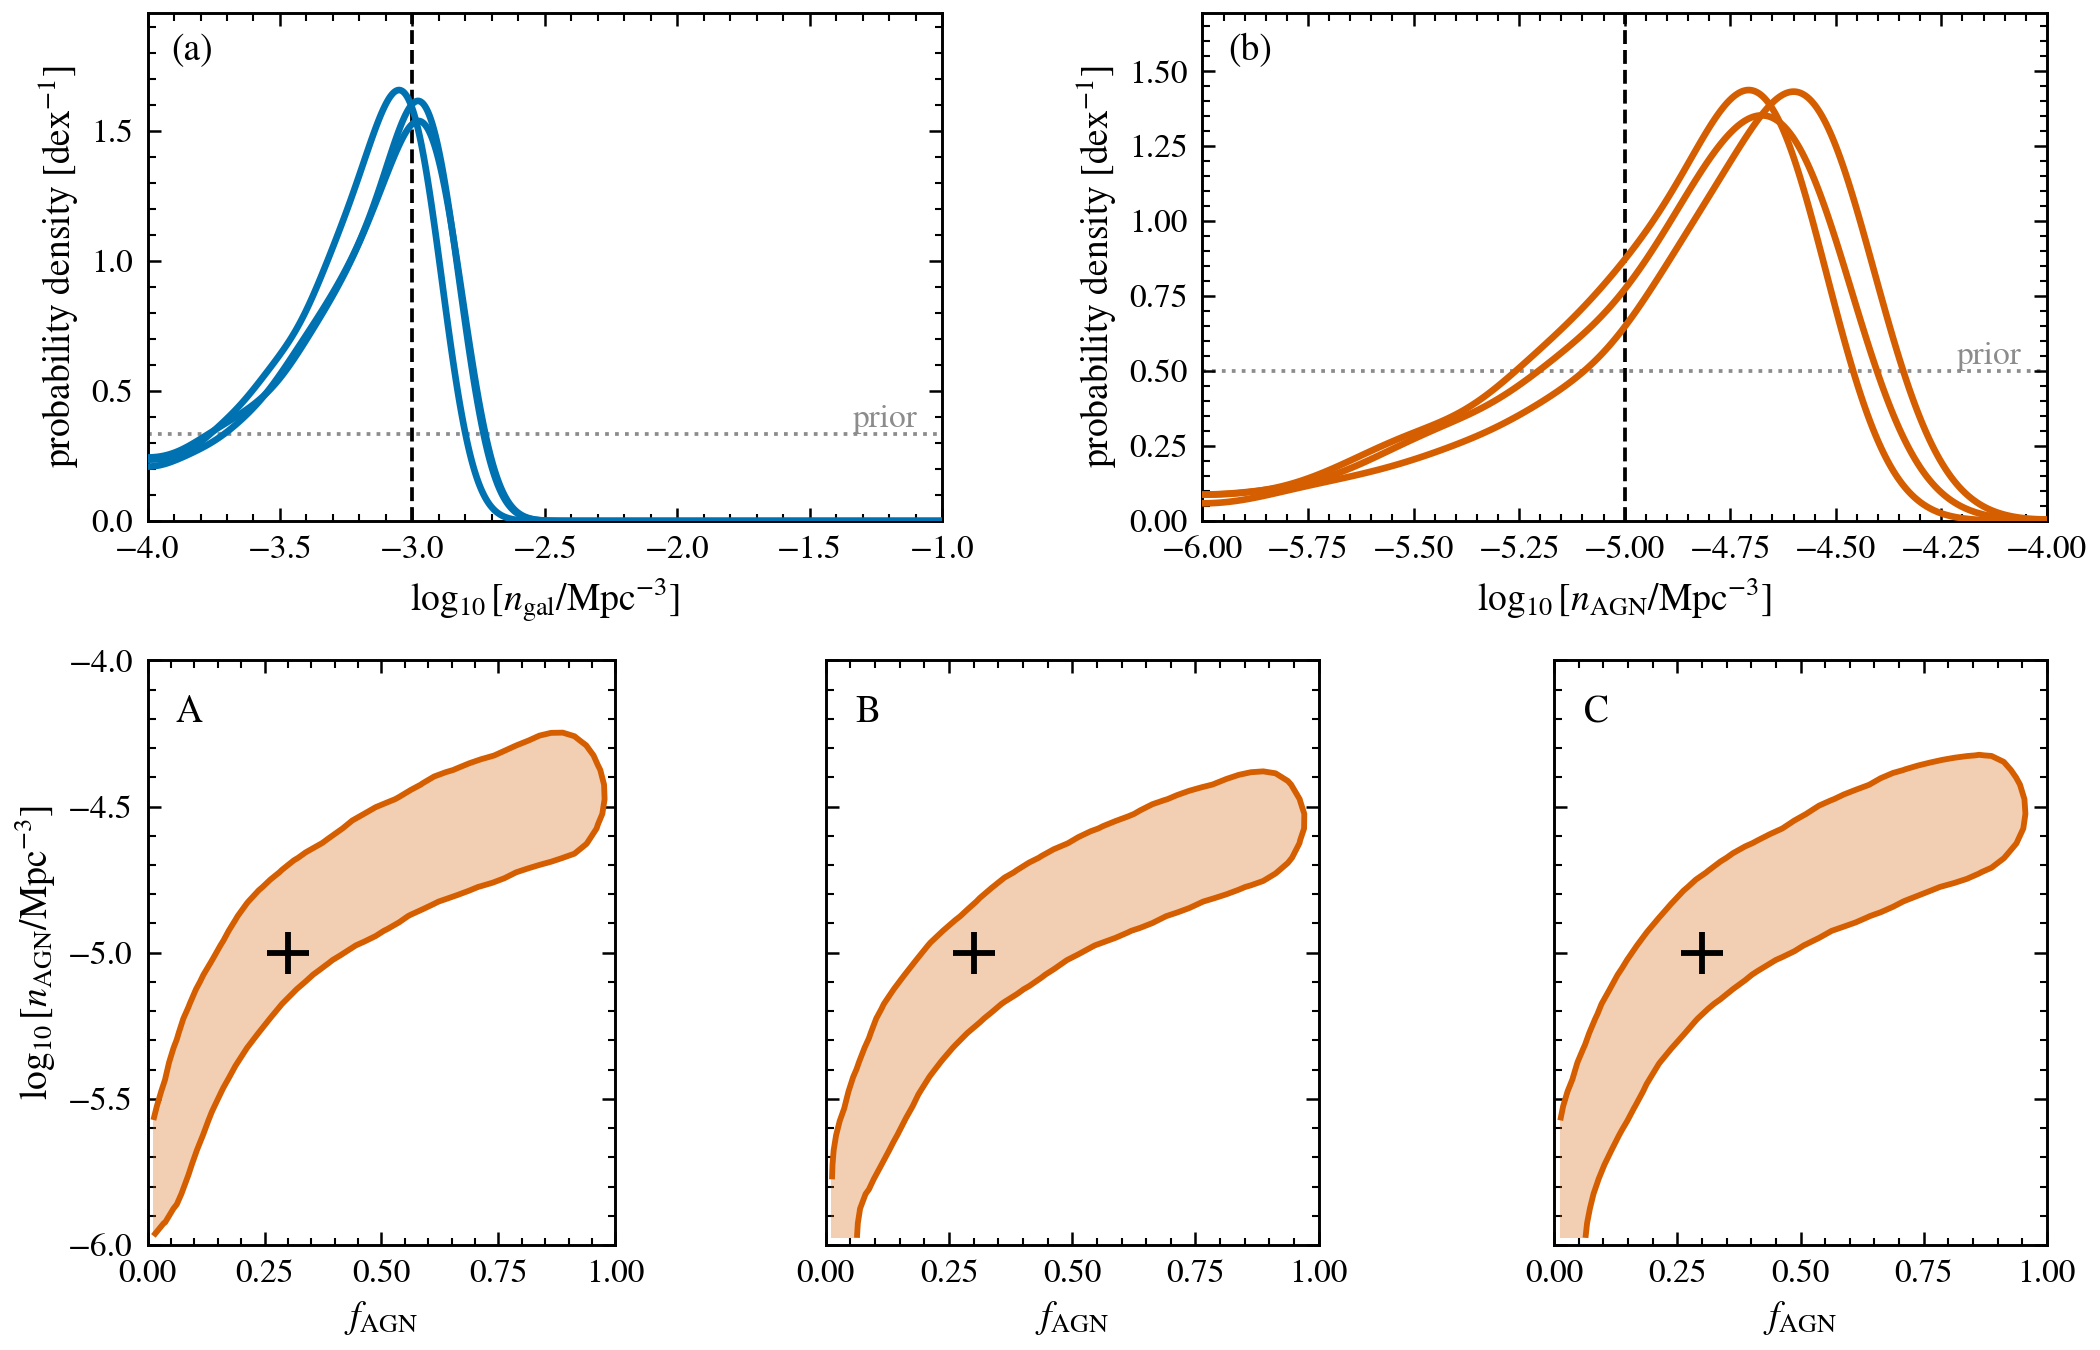
\includegraphics[width=\textwidth]{fig7_free_densities}
\caption{Number densities inferred from the mergers at \MockCompEighteen\%
completeness, together with $H_0$ and $\fagn$. (a) Posterior of the galaxy
number density and (b) of the AGN number density for three simulated
catalogs, over the full prior range; gray dotted lines are the prior
densities. Lower panels: 90\% highest-density region of $\fagn$ and the AGN
number density for catalogs A, B and C, over the full prior. Black dashed
lines and crosses are the input values. \prelim}
\label{fig:free}
\end{figure*}

%% ==========================================================================
\section{Validation}
\label{sec:validation}

The simulated catalogs of a set share one input, and their combined
posterior can be held against that input more tightly than any single
catalog (Fig.~\ref{fig:validation}). For \PureNcat{} catalogs of \MockNev{}
galaxy-hosted mergers each we find $H_0=\PureGalHzeroComb\,\kms$, with the
input at the \PureGalHzeroCombLevel\% credible level. For the same number of
catalogs of AGN-hosted mergers we find $H_0=\PureAGNHzeroComb\,\kms$: the
input \MockHzero{} lies just below the lower end of the 90\% interval,
\PureAGNHzeroCombLo, at the \PureAGNHzeroCombLevel\% level. For the
\JointNcat{} catalogs with both host classes, $H_0=\JointHzeroComb\,\kms$
and $\fagn=\JointfComb$, with the inputs at the \JointHzeroCombLevel\% and
\JointfCombLevel\% levels (Sec.~\ref{sec:two}).

\begin{figure*}
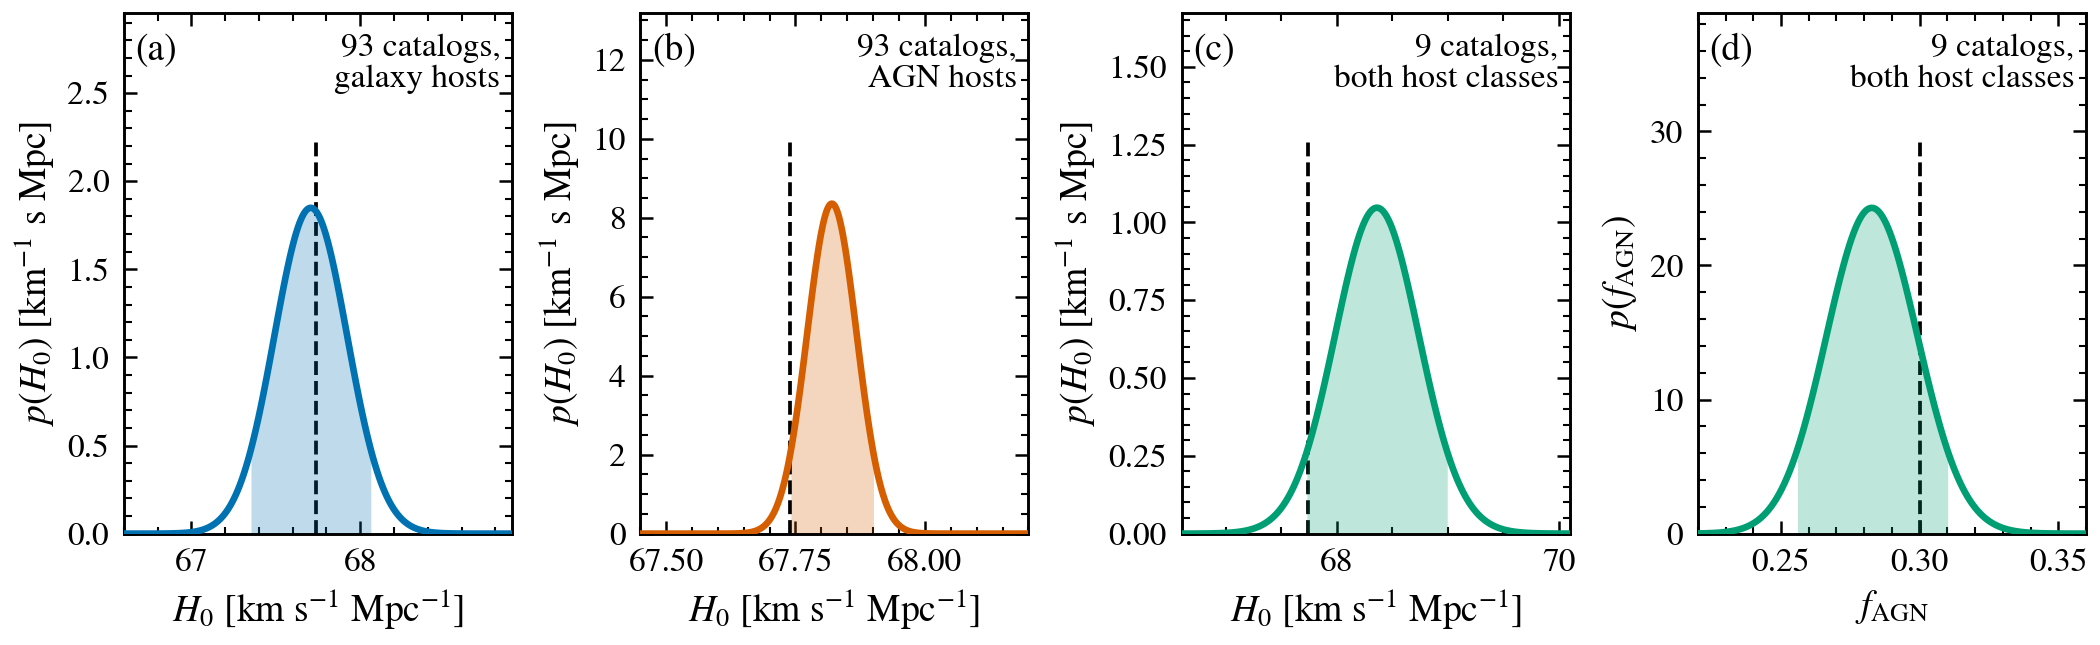
\includegraphics[width=\textwidth]{fig8_validation}
\caption{Combined posteriors over simulated catalogs, with their 90\%
intervals shaded. (a) $H_0$ from \PureNcat{} catalogs of mergers with galaxy
hosts and (b) with AGN hosts; (c) $H_0$ and (d) $\fagn$ from \JointNcat{}
catalogs with both host classes. Black dashed lines are the input values.
\prelim}
\label{fig:validation}
\end{figure*}

A model with two host classes must not find AGN-hosted mergers where there
are none. For \NullNcat{} catalogs in which every merger is hosted by a
galaxy, the combined posterior gives $\fagn<\NullfAGNUpper$ and
$H_0=\NullHzeroComb\,\kms$, with the input at the \NullHzeroLevel\% level,
and the Bayes factor of two host classes against galaxy hosts only is
$\lB=\NullLBfZero$.

The results of Secs.~\ref{sec:hd} and \ref{sec:flux} that rest on one
simulated catalog are repeated on several. At \MockCompEighteen\%
completeness and with the number densities at their inputs, \FluxNcat{}
catalogs combined give $H_0=\FluxHzeroCombEighteen\,\kms$ and
$\fagn=\FluxfCombEighteen$, with the inputs at the
\FluxHzeroCombEighteenLevel\% and \FluxfCombEighteenLevel\% levels. With
both number densities free, catalogs A, B and C combined give
$\log_{10}(\ngal/{\rm Mpc^{-3}})=\FreeLognGalEighteenComb$, with the input
at the \FreeLognGalEighteenCombLevel\% level,
$\log_{10}(\nagn/{\rm Mpc^{-3}})=\FreeLognAGNEighteenComb$,
$\fagn=\FreefAGNEighteenComb$ and $H_0=\FreeHzeroEighteenComb\,\kms$. With
host-dependent populations, \HDNcat{} catalogs combined give
$H_0=\HDEightHzeroComb\,\kms$ for the eight-parameter model, with the input
at the \HDEightHzeroCombLevel\% level, and $\CommonHzeroComb\,\kms$ for the
common population.

Every likelihood here is a Monte Carlo sum, and drawing its samples anew
moves the posterior medians by \MCShiftMedian\% of a 90\% half-width
(Appendix~\ref{app:like}).

%% ==========================================================================
\section{Conclusions}
\label{sec:conclusions}

BBH mergers in two classes of host can be told apart by where they are and
by what they are, and a measurement of $H_0$ from them has to model both. In
simulated catalogs of \MockNev{} mergers, a likelihood that assigns each
merger to a galaxy catalog or to an AGN catalog on the same density field
returns $H_0$ and $\fagn$ nearly uncorrelated, with both inputs inside the
90\% intervals of \JointNcat{} catalogs combined. If the AGN-hosted
mergers are heavier by $\MockDmuG\msun$ and one population is assumed, $H_0$
comes out $\ShiftCommonMinusFix\,\kms$ high with both catalogs and higher
with less host information. A mass peak and a spin mean for each host class
remove the bias, measure both offsets and are preferred by
$\lB=\LBOffsetsVsCommon$; the catalogs sharpen the measurement of the spin
offset by a factor of \SpinDmuChiWidthRatio, while the spins add little to
$\fagn$. This is the step that the analyses of Refs.~\cite{Bom:2023zgw,
Cross-Parkin:2026pua,Pouw:2026lar} named as their next.

What limits the measurement is not the depth of the catalogs. A flux limit
that leaves \MockCompEighteen\% of the hosts costs a factor of
\FluxHzeroRatioEighteen{} in the $H_0$ interval when the number densities
are known. The limit is that mergers measure rates per host. The fraction of
mergers in AGN needs the number of AGN in the volume to which it refers, and
a factor of two in that number moves $\fagn$ by \DeltafTwoTwentyOne, more
than its statistical uncertainty from \MockNev{} events. The mergers bound
the number density of the galaxies and not that of the AGN. $H_0$ moves by
$\DeltaHzeroTwoEighteen\,\kms$ or less for the same factor of two.

Real applications need more than our mocks contain. Our AGN are a
population of their own and not a subset of the galaxies; one luminosity
function and one isotropic flux limit serve both catalogs; every redshift is
spectroscopic; the uncataloged hosts are uniform where real ones cluster;
and hosts are weighted by number alone. The mergers are detected on a single
signal-to-noise ratio, localized to between $\MockSkyMin^\circ$ and
$\MockSkyMax^\circ$ and all lie within $z=\MockzHorizonMax$, with a mass
ratio distribution, a power-law component and a merger rate history that are
held fixed. Mergers near a supermassive black hole may also have distances
biased by their environment \cite{Li:2025eig,Liodis:2026xvs}, which we have
left out. None of this changes what Eq.~(\ref{eq:rates}) asks for. The
mergers will say how many more of them an AGN hosts than a galaxy does. How
many AGN there are, and how many of them a catalog holds, is for the surveys
to measure, and the fraction of mergers in AGN will be known as well as the
hosts the catalogs miss.

%\begin{acknowledgments}
% Funding, computing and further acknowledgments to be completed by the authors.
%\end{acknowledgments}

\appendix

\section{Likelihood evaluation}
\label{app:like}

\textit{Catalog term.} The sky is divided into equal-area pixels of HEALPix
resolution $N_{\rm side}=\MockNside$. In each pixel the first term of
Eq.~(\ref{eq:hosts}) is the sum of the kernels of its objects,
\begin{equation}
K_j(z)=\frac{\mathcal{N}(z;z_j,\sigma_j)\,dV_c/dz}
{\int_0^{z_{\rm max}}\mathcal{N}(z';z_j,\sigma_j)\,(dV_c/dz')\,dz'} ,
\label{eq:kernel}
\end{equation}
with $z_j$ the cataloged redshift and $\sigma_j=\MockDz\,(1+z_j)$. Every
object has the same weight, and a pixel with more objects carries
proportionally more probability. The completeness of a flux-limited catalog
is
\begin{equation}
C_k(z)=\frac{\Gamma\left(\alpha+1,x_{\rm lim}(z)\right)}
{\Gamma\left(\alpha+1,x_{\rm cut}\right)} ,
\label{eq:completeness}
\end{equation}
bounded to $[0,1]$, where $\Gamma$ is the incomplete gamma function,
$\alpha$ the faint-end slope of the Schechter function, $x_{\rm cut}$ the
luminosity cut of the sample in units of $L_\ast$ and $x_{\rm lim}(z)$ the
luminosity, in the same units, of an object at the flux limit at redshift
$z$. The characteristic magnitude scales with $H_0$ in such a way that $C_k$
does not depend on it.

\textit{Monte Carlo sums.} Each event has \MockNsamp{} posterior samples
$x_{ij}$, drawn under a prior $p_{\rm PE}$, and the detected fraction is
estimated from simulated signals drawn from a density $p_{\rm draw}$ and
passed through the detection rule of the events. With
$w_{ij}=\pi(x_{ij}|\Lambda)/p_{\rm PE}(x_{ij})$, the estimate of
Eq.~(\ref{eq:like}) is
\begin{equation}
\ln\hat\Lcal=\sum_{i=1}^{N}\ln\bigg[\frac{1}{n}\sum_{j=1}^{n}w_{ij}\bigg]
-N\ln\hat\mu+\frac{N(N+3)}{2N_{\rm eff}} ,
\label{eq:estimator}
\end{equation}
where $\hat\mu$ is the mean of $\pi/p_{\rm draw}$ over all drawn signals,
counted as zero for those not detected, $N_{\rm eff}$ is the effective
number of detected signals, and the last term corrects for the uncertainty
of $\hat\mu$ \cite{Farr:2019rap}. For the reference catalog $\MockNinjDrawn$
signals are drawn and $\MockNinjFound$ are detected. They come from a
mixture of the input population, a broad distribution and a component
concentrated on the cataloged AGN, so that the sparse AGN term of the
detected fraction is sampled at every $H_0$ of the prior. A point of
parameter space is admitted only if $N_{\rm eff}>\NeffFactor N$.

\textit{Accuracy.} The variance of $\ln\hat\Lcal$ is the sum of the
variances of the event terms and $N^2/N_{\rm eff}$. At the maximum of the
posterior it is between \JointLnLVarMin{} and \JointLnLVarMax{} for the
\JointNcat{} catalogs of Sec.~\ref{sec:two} and \LnLVarAGNHosted{} for the
AGN-hosted sets, where few posterior samples of an event fall on the narrow
kernels of the sparse catalog; the eight-parameter model admits only points
with a variance below \VarCapEight. Analyses of the observed catalogs limit this variance to one
\cite{LIGOScientific:2025pvj}, following
Refs.~\cite{Essick:2022ojx,Talbot:2023pex}. We measure its
effect directly, by drawing the posterior samples and the simulated signals
anew and repeating the analysis: the posterior medians move by
\MCShiftMedian\% of a 90\% half-width and the widths change by
\MCWidthChange\%, and by \MCWidthChangeAGN\% for the AGN-hosted sets.

\section{Measurement model of the mock events}
\label{app:pe}

The optimal signal-to-noise ratio of a merger with redshifted chirp mass
$\mathcal{M}_z$ at luminosity distance $d_L$ is
\begin{equation}
\rho=\MockRhoRef\left(\frac{\mathcal{M}_z}{\MockMcRef\msun}\right)^{5/6}
\frac{1\,{\rm Gpc}}{d_L} ,
\label{eq:snr}
\end{equation}
and the data of an event are
\begin{equation}
\begin{split}
\rho_{\rm obs}&=\rho+\epsilon_\rho ,\\
\ln\mathcal{M}_{z,{\rm obs}}&=\ln\mathcal{M}_z+\sigma_{\mathcal{M}}\,\epsilon_{\mathcal{M}} ,\\
\ln q_{\rm obs}&=\ln q+\sigma_q\,\epsilon_q ,\\
\chi_{\rm eff,obs}&=\chieff+\sigma_\chi^{\rm obs}\,\epsilon_\chi ,
\end{split}
\label{eq:data}
\end{equation}
with independent unit Gaussian variables $\epsilon$ and widths
$(\sigma_{\mathcal{M}},\sigma_q,\sigma_\chi^{\rm obs})=
(\MockSigLnMc,\MockSigLnq,\MockSigChi)\times\MockSNRthr/\rho_{\rm obs}$. The
declination is observed with a Gaussian error $\sigma_{\rm
sky}=\MockSkyCoeff^\circ/\rho_{\rm obs}$, bounded between
$\MockSkyClipLo^\circ$ and $\MockSkyClipHi^\circ$, and the right ascension
with that error divided by the cosine of the observed declination. An event is detected when
$\rho_{\rm obs}\geq\MockSNRthr$. No observed value is truncated.

Every width depends on $\rho_{\rm obs}$ alone, so for a prior that is flat
in $(\ln\mathcal{M}_z,\ln q,\rho,\chieff)$ and in the sky position the
posterior is a product of Gaussians centered on the observed values, with
the same widths and restricted to $q\leq1$, $\rho>0$ and $|\chieff|\leq1$.
The \MockNsamp{} samples of an event are drawn from it and mapped to the
redshifted primary mass $m_{1z}$, $q$, $d_L$ and $\chieff$ through
Eq.~(\ref{eq:snr}). In these variables the prior density is
\begin{equation}
p_{\rm PE}(m_{1z},q,d_L,\chieff)\propto\frac{\rho}{d_L\,m_{1z}\,q} ,
\label{eq:ppe}
\end{equation}
which is the density that the weights of Eq.~(\ref{eq:estimator}) divide
out.

\section{Posterior of the eight-parameter model}
\label{app:corner}

Figure~\ref{fig:corner} shows the posterior of the host-dependent model with
the reference peak location, the reference spin mean, both widths and both
offsets free together with $H_0$ and $\fagn$ (Sec.~\ref{sec:hd}).

\begin{figure*}
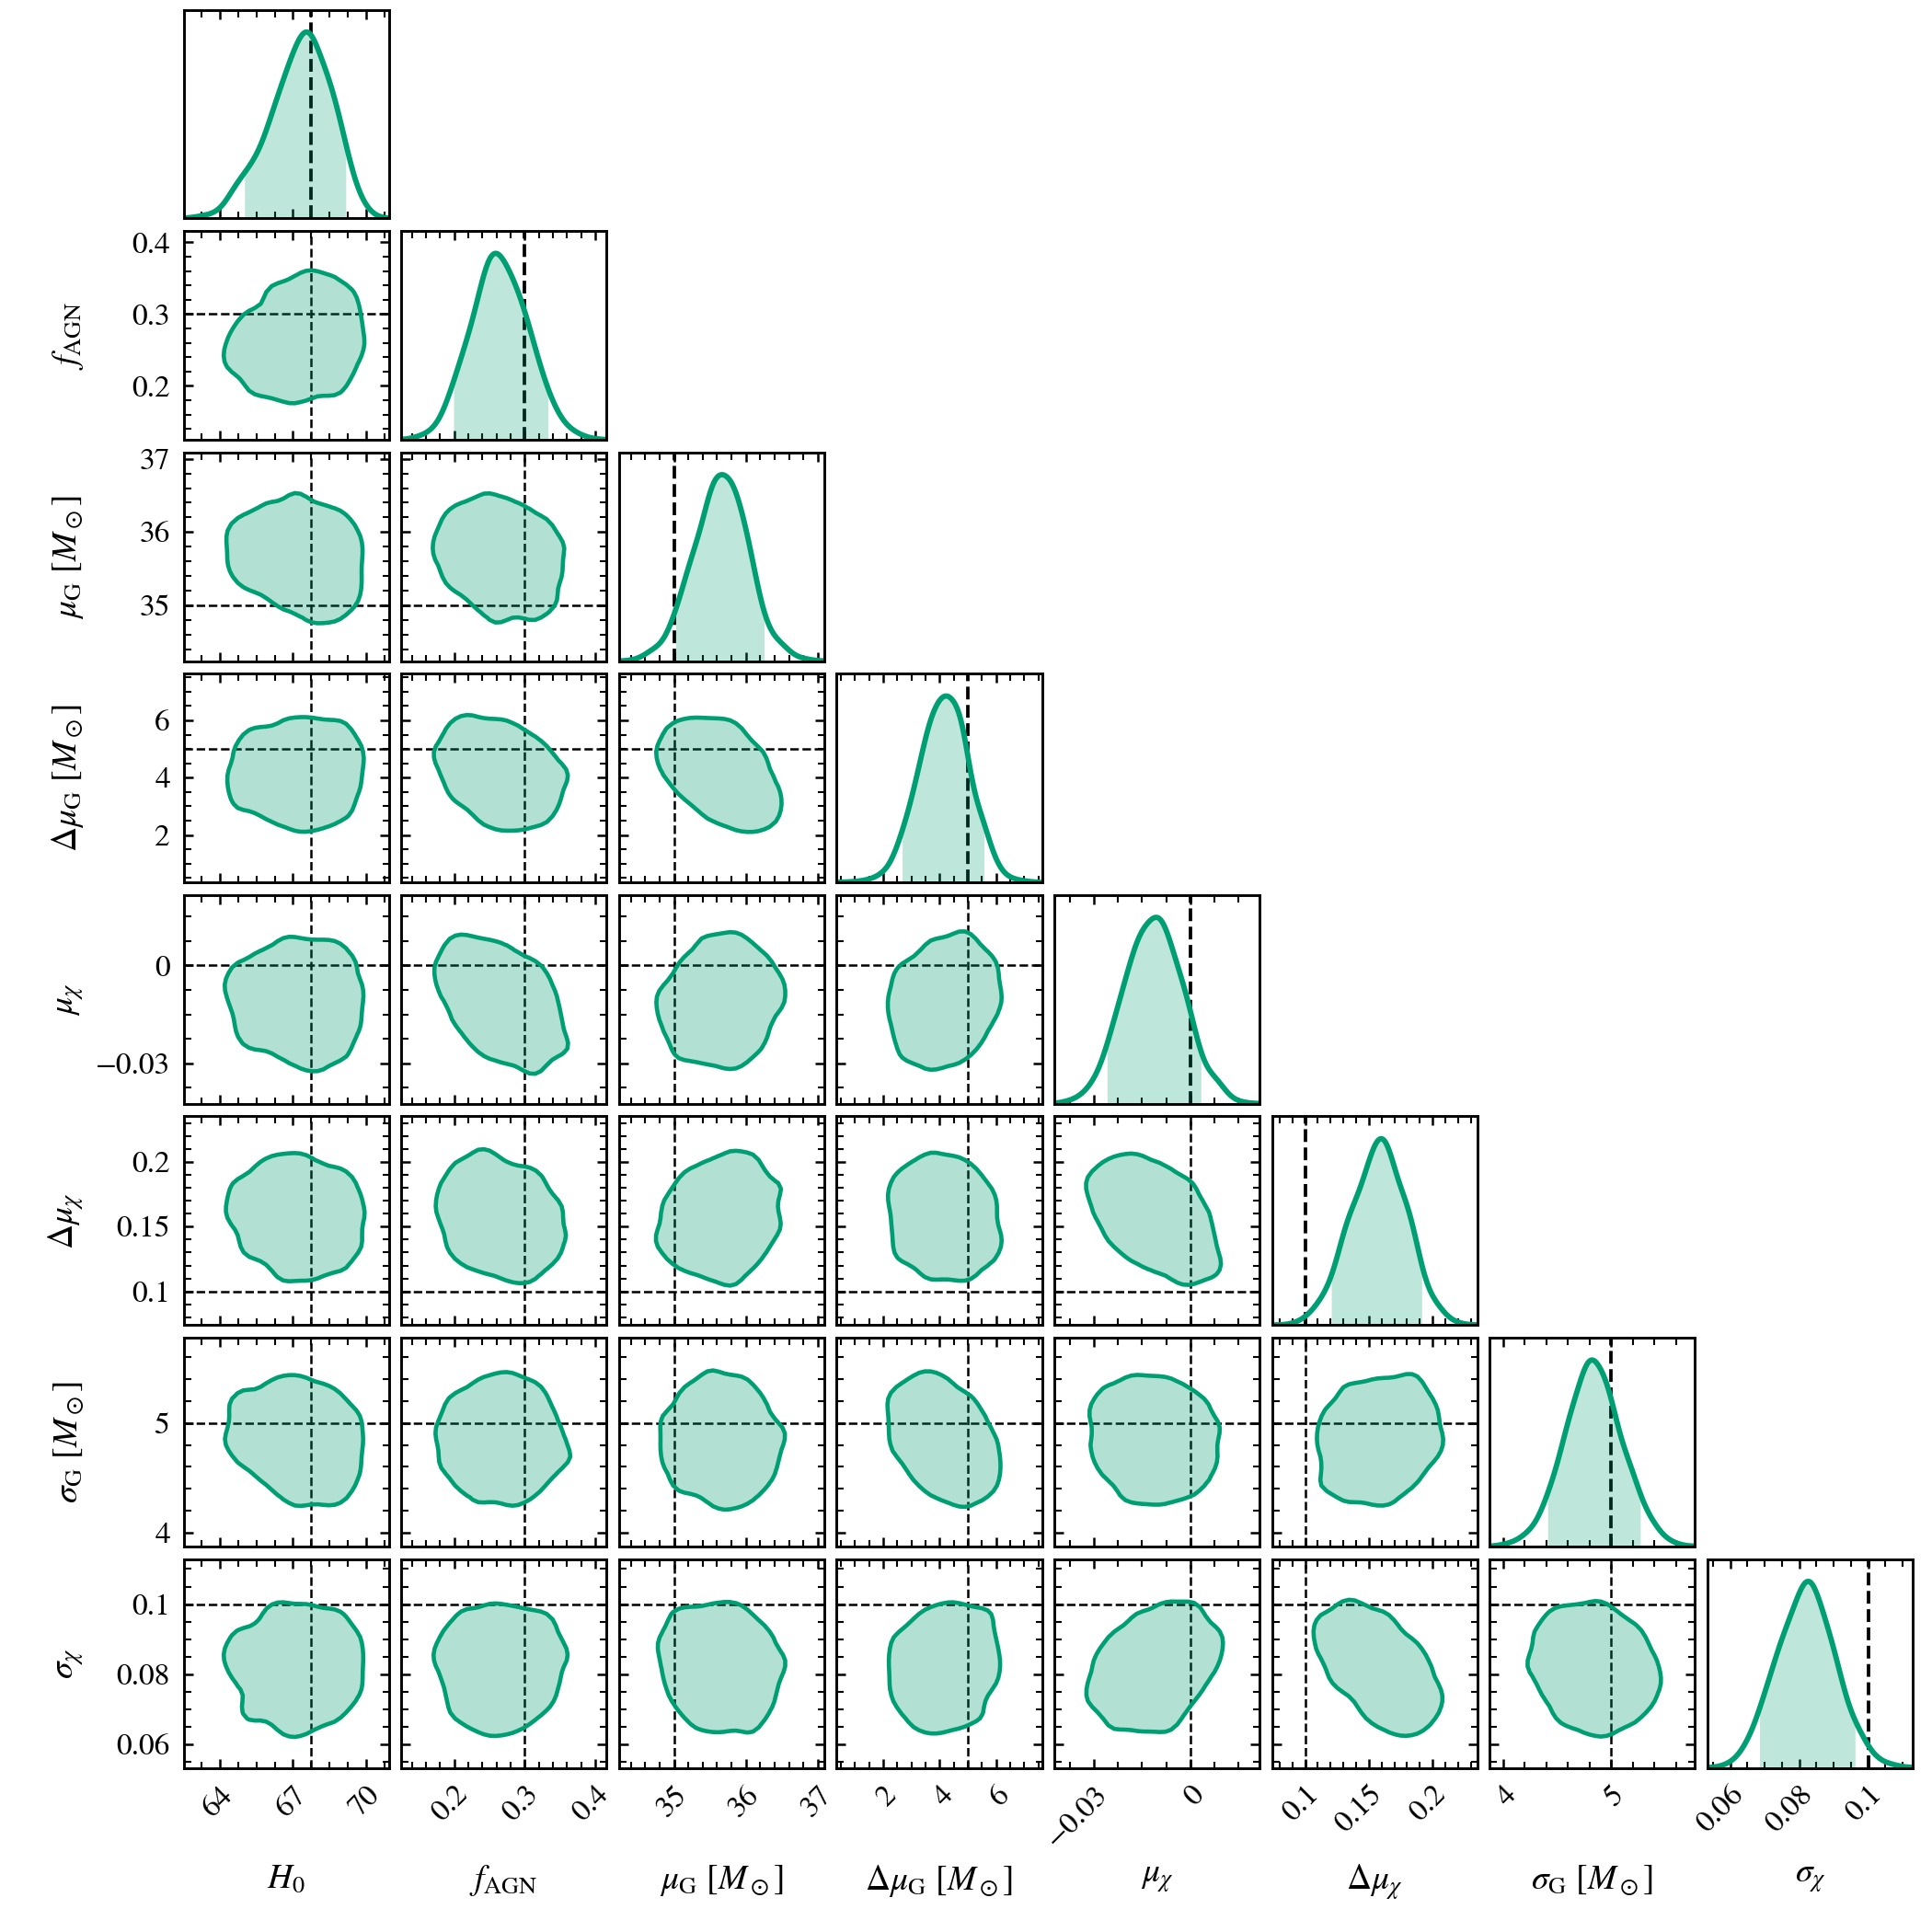
\includegraphics[width=\textwidth]{figC1_corner}
\caption{Posterior of the eight-parameter host-dependent model on the
host-dependent mock with both catalogs (one simulated catalog). Diagonal
panels show posterior densities with their 90\% intervals shaded, and the
other panels 90\% highest-density regions; the axes are cropped to the
posterior. Black dashed lines are the input values. \prelim}
\label{fig:corner}
\end{figure*}

\bibliography{refs}

\end{document}
